%%%%%%%%%%%%%%%%%%%%%%%%%%%%%%%%%%%%%%%%%
% Diaz Essay
% LaTeX Template
% Version 2.0 (13/1/19)
%
% This template originates from:
% http://www.LaTeXTemplates.com
%
% Authors:
% Vel (vel@LaTeXTemplates.com)
% Nicolas Diaz (nsdiaz@uc.cl)
%
% License:
% CC BY-NC-SA 3.0 (http://creativecommons.org/licenses/by-nc-sa/3.0/)
%
%%%%%%%%%%%%%%%%%%%%%%%%%%%%%%%%%%%%%%%%%

%----------------------------------------------------------------------------------------
%    PACKAGES
%----------------------------------------------------------------------------------------
\documentclass[11pt, table]{diazessay} % Font size (can be 10pt, 11pt or 12pt)

\usepackage{graphicx}
\usepackage{anyfontsize}
\usepackage{tikz}
\usetikzlibrary{calc}
\usepackage[hyphens]{url}

\usepackage[
	type={CC},
	modifier={by-nc-sa},
	version={3.0},
]{doclicense}


%----------------------------------------------------------------------------------------
%    LINK COLORS
%----------------------------------------------------------------------------------------
\usepackage{hyperref}
\usepackage[]{xcolor}
\hypersetup{colorlinks=true,urlcolor=blue,linkcolor=blue, citecolor=blue}
%% or
% \hypersetup{colorlinks=false,pdfborder=000}
% hack into hyperref
\makeatletter
\DeclareUrlCommand\ULurl@@{%
  \def\UrlFont{\ttfamily\color{blue}}%
  \def\UrlLeft{\uline\bgroup}%
  \def\UrlRight{\egroup}}
\def\ULurl@#1{\hyper@linkurl{\ULurl@@{#1}}{#1}}
\DeclareRobustCommand*\ULurl{\hyper@normalize\ULurl@}
\makeatother

%----------------------------------------------------------------------------------------
%    FORMAL QUOTES
%----------------------------------------------------------------------------------------
% for adjustwidth environment
\usepackage[strict]{changepage}

% for formal definitions
\usepackage{framed}

% environment derived from framed.sty: see leftbar environment definition
\definecolor{formalshade}{rgb}{0.95,0.95,1}

\newenvironment{formal}{%
  \def\FrameCommand{%
	\hspace{1pt}%
	{\color{w_lightblue}\vrule width 2pt}%
	{\color{formalshade}\vrule width 4pt}%
	\colorbox{formalshade}%
  }%
  \MakeFramed{\advance\hsize-\width\FrameRestore}%
  \noindent\hspace{-4.55pt}% disable indenting first paragraph
  \begin{adjustwidth}{}{7pt}%
  \vspace{2pt}\vspace{2pt}%
}
{%
  \vspace{2pt}\end{adjustwidth}\endMakeFramed%
}

%----------------------------------------------------------------------------------------
%    BIBLIOGRAPHY STYLE
%----------------------------------------------------------------------------------------

\usepackage[numbers]{natbib} % bibliography style

\usepackage{amsmath, amssymb, latexsym}
\usepackage{minted} % code formatting
\usemintedstyle{borland}

%----------------------------------------------------------------------------------------
%    TIKZ
%----------------------------------------------------------------------------------------

 % 3D plots and tikz images
\usepackage{tikz}
\usepackage{tikz-3dplot}
\usetikzlibrary{shapes,arrows,chains,positioning,shapes.geometric,arrows.meta,backgrounds,fit, shapes, calc, matrix}

\usepackage{forest} % trees
\usepackage{float}

\newcommand{\empt}[2]{$#1^{\langle #2 \rangle}$}
%----------------------------------------------------------------------------------------
%    IMAGE SHAPES
%----------------------------------------------------------------------------------------
% Define block styles
\tikzstyle{decision} = [diamond, draw, fill=w_lightblue,
	text width=4.5em, text badly centered, node distance=3cm, inner sep=0pt]
\tikzstyle{block} = [rectangle, draw, fill=w_lightblue,
	text width=5em, text centered, rounded corners, minimum height=4em]
\tikzstyle{line} = [draw, -latex']
\tikzstyle{cloud} = [draw, ellipse,fill=red!20, node distance=3cm,
	minimum height=2em]
	\tikzstyle{mybox} = [draw=red, fill=w_lightblue, very thick,
	rectangle, rounded corners, inner sep=10pt, inner ysep=20pt]
\tikzstyle{fancytitle} =[fill=red, text=white]
\usepackage{tikzscale}
\usepackage{adjustbox}

%----------------------------------------------------------------------------------------
%    TOC
%----------------------------------------------------------------------------------------
\setcounter{secnumdepth}{4} % how many sectioning levels to assign numbers to
\setcounter{tocdepth}{3}	% how many sectioning levels to show in ToC

%----------------------------------------------------------------------------------------
%    CAPTIONS
%----------------------------------------------------------------------------------------

\usepackage{subcaption}
\DeclareCaptionFormat{custom}
{%
	\textbf{#1#2}\textit{\small #3}
}
\captionsetup{format=custom}
%----------------------------------------------------------------------------------------
%    MATRIX
%----------------------------------------------------------------------------------------
\definecolor{dgreen}{RGB}{72,127,30}
\makeatletter
\tikzset{matrix dividers/.style={execute at end matrix={
\foreach \XX in {2,...,\the\pgf@matrix@numberofcolumns}
{\draw[#1] ($(\tikz@fig@name-1-\XX)!0.5!(\tikz@fig@name-1-\the\numexpr\XX-1)$)
coordinate (aux) (aux|-\tikz@fig@name.north)
 --  (aux|-\tikz@fig@name.south);
}
\foreach \XX in {2,...,\the\pgfmatrixcurrentrow}
{\draw[#1] ($(\tikz@fig@name-\XX-1)!0.5!(\tikz@fig@name-\the\numexpr\XX-1\relax-1)$)
coordinate (aux) (aux-|\tikz@fig@name.west)
 --  (aux-|\tikz@fig@name.east);
}
}},matrix frame/.style={execute at end matrix={
\draw[#1] (\tikz@fig@name.south west) rectangle (\tikz@fig@name.north east);
}}}
% from https://tex.stackexchange.com/a/386805/121799
\def\tikz@lib@matrix@empty@cell{\iftikz@lib@matrix@empty\node[name=\tikzmatrixname-\the\pgfmatrixcurrentrow-\the\pgfmatrixcurrentcolumn,empty node]{};\fi}
\makeatother
\tikzset{matrix of mathsf nodes/.style={%
  matrix of nodes,
  nodes={%
   execute at begin node=$\mathsf\bgroup,%
   execute at end node=\egroup$%
  }%
}}

\usepackage{tikz-qtree,tikz-qtree-compat}


%----------------------------------------------------------------------------------------
%    COLORS
%----------------------------------------------------------------------------------------

\definecolor{w_lightblue}{HTML}{D5E7F7}
\definecolor{lightblue}{HTML}{ADD8E6}
\definecolor{celestialblue}{rgb}{0.29, 0.59, 0.82}
\definecolor{asparagus}{rgb}{0.53, 0.66, 0.42}
\definecolor{azure}{rgb}{0.0, 0.5, 1.0}
%----------------------------------------------------------------------------------------
%    TITLE SECTION
%----------------------------------------------------------------------------------------
\begin{document}
\begin{sloppypar}

\thispagestyle{empty}

\thispagestyle{empty}

\begin{tikzpicture}[overlay,remember picture]

% Background color
\fill[black!2] (current page.south west) rectangle (current page.north east);

% Image
\node at ($(current page.north)+(0,-1/2.5*\paperheight)$) {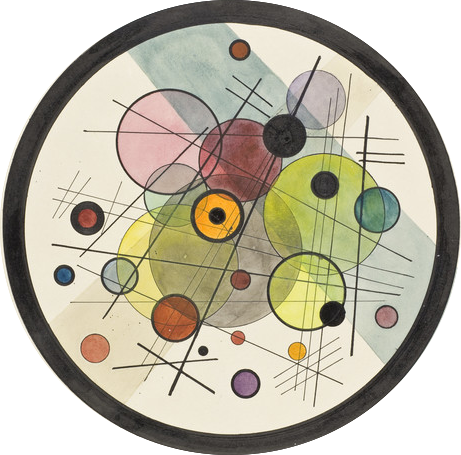
\includegraphics[width=0.5\textwidth]{figures/kandinsky.png}};

% Title
\node[align=center] at ($(current page.center)+(0,-5)$)
{
{\fontsize{40}{44} \selectfont {What are embeddings}} \\[1cm]
\rule[0.5ex]{4cm}{0.4pt} \\[1cm]
{\fontsize{30}{19.2} \selectfont \textcolor{blue}{\bfseries Vicki Boykis}}\\[3pt]

};


\end{tikzpicture}


\newpage

%----------------------------------------------------------------------------------------
%    ABSTRACT AND META
%----------------------------------------------------------------------------------------

\begin{abstract}
Over the past decade, embeddings --- numerical representations of machine learning features used as input to deep learning models --- have become a foundational data structure in industrial machine learning systems. TF-IDF, PCA, and one-hot encoding have always been key tools in machine learning systems as ways to compress and make sense of large amounts of textual data.  However, traditional approaches were limited in the amount of context they could reason about with increasing amounts of data. As the volume, velocity, and variety of data captured by modern applications has exploded, creating approaches specifically tailored to scale has become increasingly important.

Google's \href{https://arxiv.org/abs/1301.3781}{Word2Vec paper} made an important step in moving from simple statistical representations to semantic meaning of words. The subsequent rise of the \href{https://arxiv.org/abs/1706.03762}{Transformer architecture} and transfer learning, as well as the latest surge in generative methods has enabled the growth of embeddings as a foundational machine learning data structure. This survey paper aims to provide a deep dive into what embeddings are, their history, and usage patterns in industry.

\end{abstract}

\section*{Colophon }
This paper is typeset with \LaTeX. The cover art is Kandinsky's "Circles in a Circle" , 1923. \href{https://vickiboykis.com/2023/02/26/what-should-you-use-chatgpt-for/}{ChatGPT was used} to generate some of the figures.

\section*{Code, \LaTeX, and Website}
The latest version of the paper and code examples \href{https://github.com/veekaybee/what_are_embeddings}{are available here.} The   \href{http://vickiboykis.com/what_are_embeddings/}{website for this project is here.}

\section*{About the Author}
Vicki Boykis is a machine learning engineer. Her website is \href{https://www.vickiboykis.com}{vickiboykis.com} and her semantic search side project is \href{https://viberary.pizza}{viberary.pizza}. 

%----------------------------------------------------------------------------------------
%    CREATIVE COMMONS LICENSE
%----------------------------------------------------------------------------------------

\section*{Acknowledgements}
I'm grateful to everyone who has graciously offered technical feedback but especially to Nicola Barbieri, Peter Baumgartner, Luca Belli, James Kirk, and Ravi Mody. All remaining errors, typos, and bad jokes are mine. Thank you to Dan for your patience, encouragement, for parenting while I was in the latent space, and for once casually asking, "How do you generate these 'embeddings', anyway?"

\section*{License}
\doclicenseThis
\newpage

%----------------------------------------------------------------------------------------
%    TOC
%----------------------------------------------------------------------------------------
\tableofcontents
\newpage

%----------------------------------------------------------------------------------------
%	ESSAY BODY
%----------------------------------------------------------------------------------------

\section{Introduction}

Implementing deep learning models has become an increasingly important machine learning strategy\footnote{Check out the machine learning industrial view Matt Turck \href{https://mattturck.com/mad2023/}{puts together every year, which has exploded in size.}} for companies looking to build data-driven products. In order to build and power deep learning models, companies collect and feed hundreds of millions of terabytes of multimodal\footnote{Multimodal means a variety of data usually including text, video, audio, and more recently as shown in \href{https://ai.facebook.com/blog/imagebind-six-modalities-binding-ai/}{Meta's ImageBind}, depth, thermal, and IMU.} data into deep learning models. As a result, \textbf{embeddings} --- deep learning models' internal representations of their input data --- are quickly becoming a critical component of building machine learning systems.

For example, they make up a significant part of Spotify's item recommender systems  \citep{hansen2020contextual}, YouTube video recommendations of what to watch  \citep{covington2016deep}, and Pinterest's visual search  \citep{jing2015visual}. Even if they are not explicitly presented to the user through recommendation system UIs, embeddings are also used internally at places like Netflix to make content decisions around which shows to develop based on user preference popularity.

\begin{figure}[H]
\centering{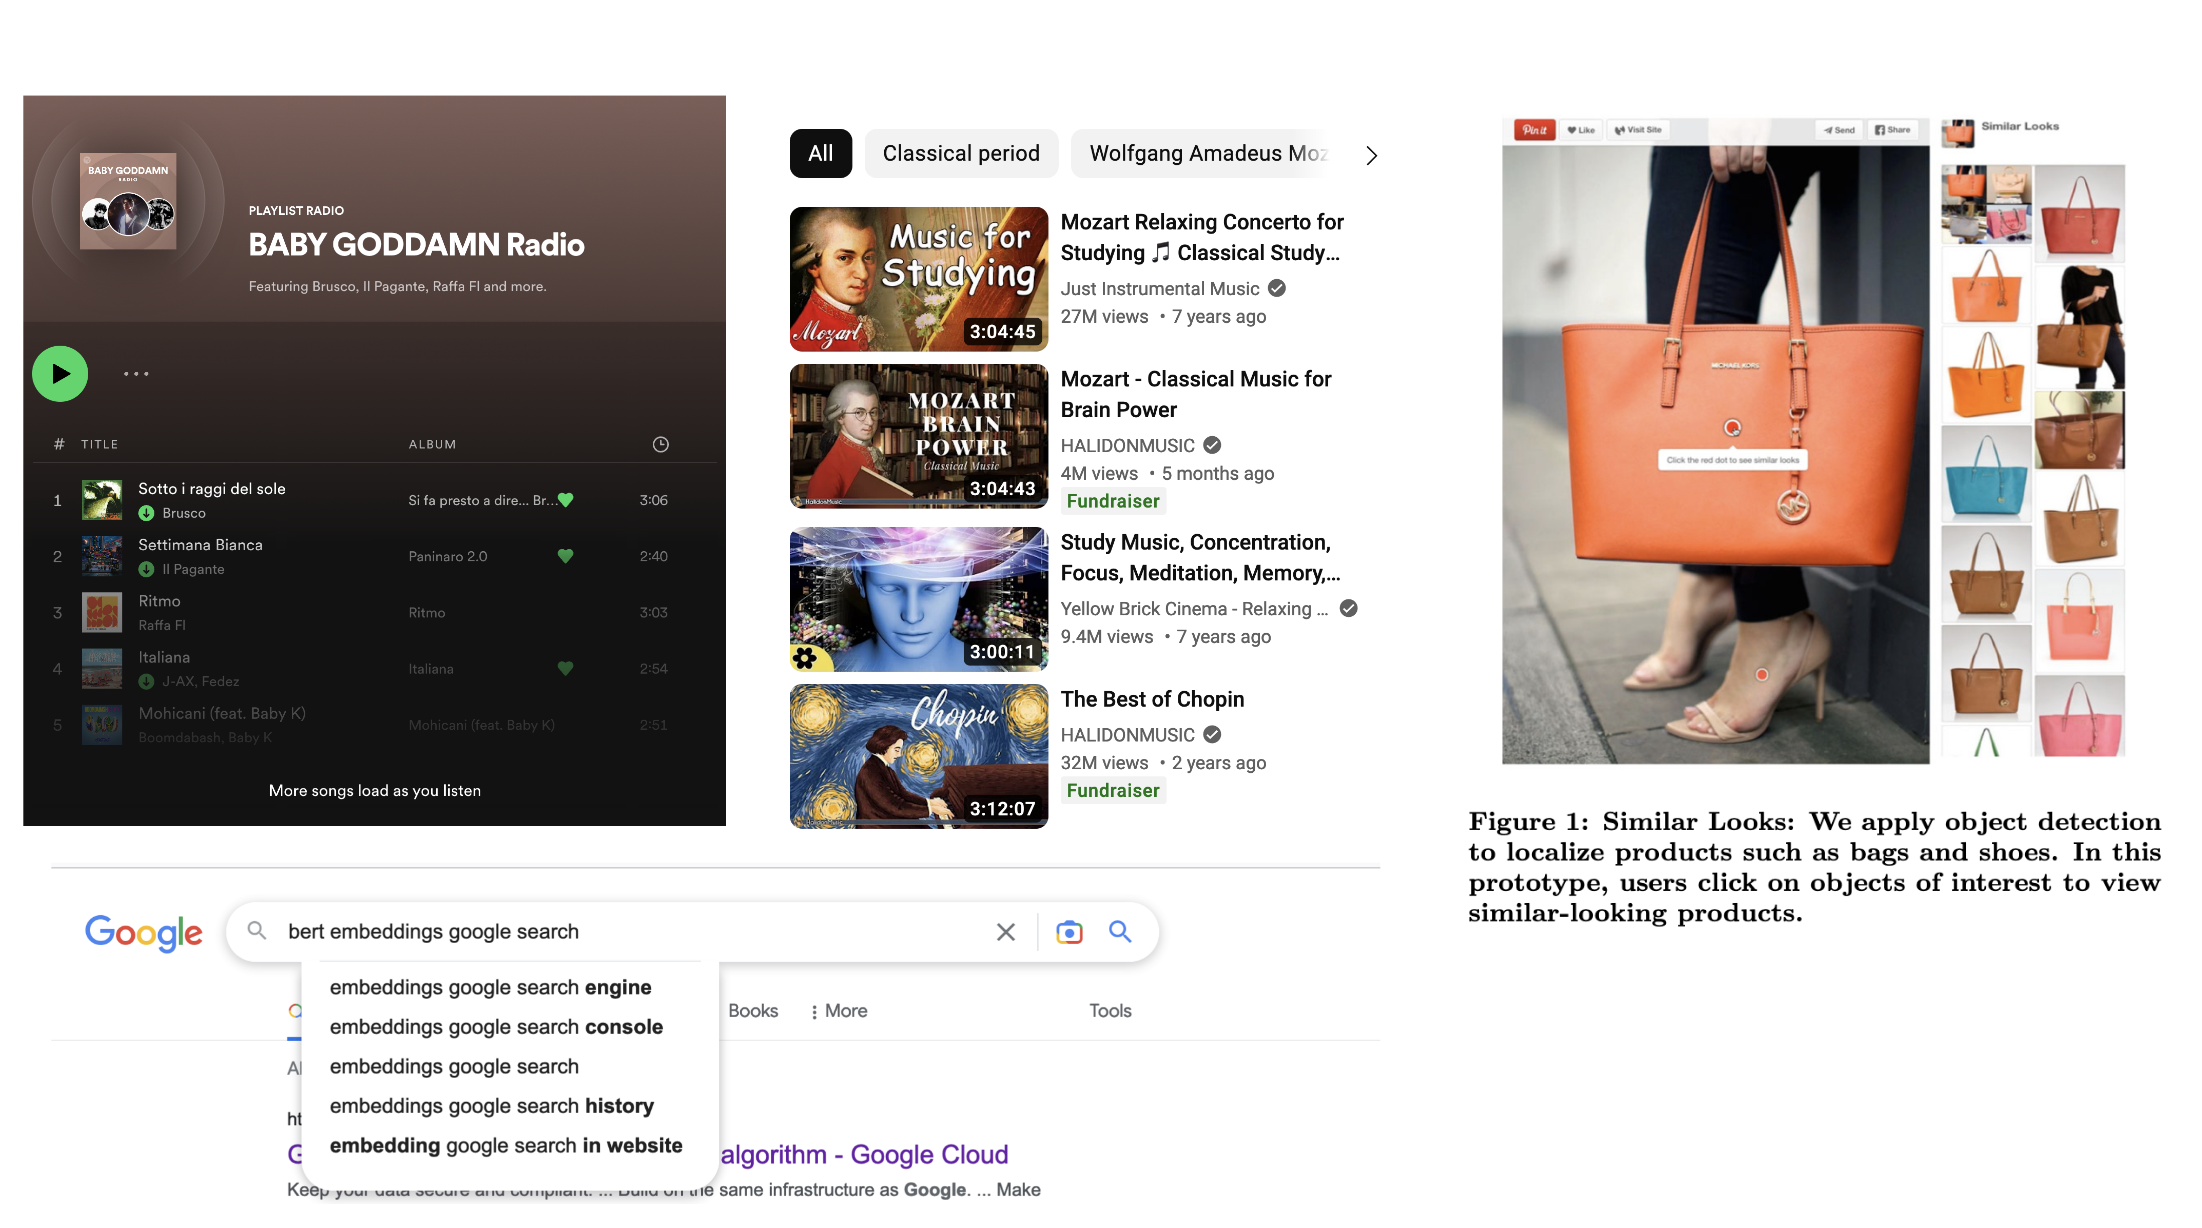
\includegraphics[width=\textwidth]{figures/embeddings.png}}
\caption{Left to right: Products that use embeddings used to generate recommended items: Spotify Radio, YouTube Video recommendations, visual recommendations at Pinterest, BERT Embeddings in suggested Google search results}
\end{figure}

The usage of embeddings to generate compressed, context-specific representations of content exploded in popularity after the publication of Google’s Word2Vec paper  \citep{mikolov2013efficient}.

\begin{figure}[H]
\centering
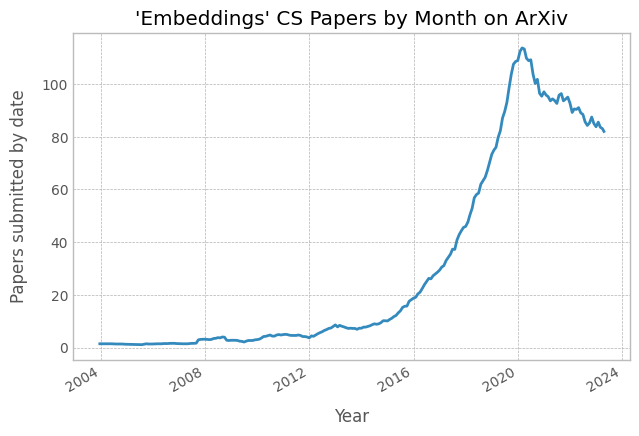
\includegraphics[width=.7\linewidth]{figures/embeddings_1.png}
\caption{Embeddings papers in Arxiv by month. It's interesting to note the decline in frequency of embeddings-specific papers, possibly in tandem with the rise of deep learning architectures like GPT \href{https://github.com/veekaybee/what_are_embeddings/blob/main/notebooks/fig_2_embeddings_papers.ipynb}{source}}
\end{figure}

Building and expanding on the concepts in Word2Vec, the Transformer  \citep{vaswani2017attention} architecture, with its self-attention mechanism, a much more specialized case of calculating context around a given word, has become the de-facto way to learn representations of growing multimodal vocabularies, and its rise in popularity both in academia and in industry has caused embeddings to become a staple of deep learning workflows.

However, the concept of embeddings can be elusive because they're neither data flow inputs or output results - they are intermediate elements that live within machine learning services to refine models. So it's helpful to define them explicitly from the beginning.

As a general definition, embeddings are data that has been transformed into n-dimensional matrices for use in deep learning computations. The process of embedding (as a verb):  
\begin{formal}
\begin{itemize}
   \item \emph{Transforms} multimodal input into representations that are easier to perform intensive computation on, in the form of \textbf{vectors}, tensors, or graphs \citep{rao2019natural}. For the purpose of machine learning, we can think of vectors as a list (or array) of numbers.
  \item \emph{Compresses} input information for use in a machine learning \textbf{task} --- the type of methods available to us in machine learning to solve specific problems --- such as summarizing a document or identifying tags or labels for social media posts or performing \textbf{semantic search} on a large text corpus. The process of compression changes variable feature dimensions into fixed inputs, allowing them to be passed efficiently into downstream components of machine learning systems.
  \item \emph{Creates an embedding space} that is specific to the data the embeddings were trained on but that, in the case of deep learning representations, can also generalize to other tasks and domains through \textbf{transfer learning} --- the ability to switch contexts --- which is one of the reasons embeddings have exploded in popularity across machine learning applications
\end{itemize}
\end{formal}

What do embeddings actually look like? Here is one single embedding, also called a \textbf{vector}, in three \textbf{dimensions}. We can think of this as a representation of a single element in our dataset. For example, this hypothetical embedding represents a single word "fly", in three dimensions.  Generally, we represent individual embeddings as row vectors.

\begin{equation}
\begin{bmatrix}
1 & 4 & 9
\end{bmatrix}
\end{equation}


And here is a \textbf{tensor}, also known as a \textbf{matrix}\footnote{The difference between a matrix and a tensor is that it's a matrix if you're doing linear algebra and a tensor if you're an AI researcher.}, which is a multidimensional combination of vector representations of multiple elements. For example, this could be the representation of "fly", and "bird."

\begin{equation}
\begin{bmatrix}
1 & 4 & 9\\
4 & 5 & 6
\end{bmatrix}
\end{equation}

These embeddings are the output of the process of \textbf{learning} embeddings, which we do by passing raw input data into a machine learning model. We transform that multidimensional input data by compressing it, through the algorithms we discuss in this paper, into a lower-dimensional space. The result is a set of vectors in an \textbf{embedding space.}  

\begin{figure}[H]
    \centering
    \begin{tikzpicture}[node distance=4cm]
   	 \node[draw, rectangle] (multimodal) at (0,0) [block] {
   		 \begin{tabular}{c}
       		 Word \\
       		 Sentence \\
       		 Image
   		 \end{tabular}
   	 };
   	 \node[above] at (multimodal.north) {Multimodal data} [block];

   	 \node[draw, rectangle, right of=multimodal, xshift=3cm] (embedding) [block] {
   		 \begin{tabular}{c}
      		 $[1,4,9]$ \\
      		 $ [1,4,7]$ \\
      		 $ [12,0,3]$
   		 \end{tabular}
   	 };
		 \node[above] at (embedding.north) {Embedding Space} [block];

   	 \draw[->] (multimodal) -- node[above] {Algorithm } (embedding);
    \end{tikzpicture}
    \caption{The process of embedding.}
    \label{fig:embedding}
\end{figure}

We often talk about item embeddings being in $X$ dimensions, ranging anywhere from 100 to 1000, with diminishing returns in usefulness somewhere beyond 200-300 in the context of using them for machine learning problems\footnote{Embedding size is tunable as a hyperparameter but so far there have only been a \href{https://aclanthology.org/I17-2006.pdf}{few papers on optimal embedding size, with most of the size of embeddings set through magic and guesswork}}. This means that each item (image, song, word, etc) is represented by a vector of length $X$, where each value is a coordinate in an $X$-dimensional space.

We just made up an embedding for "bird", but let's take a look at what a real one for the word "hold" would look like in the quote, as generated by the BERT deep learning model,

\begin{formal}"Hold fast to dreams, for if dreams die, life is a broken-winged bird that cannot fly." --- Langston Hughes
\end{formal}

We've highlighted this quote because we'll be working with this sentence as our input example throughout this text.

\begin{figure}[H]
\begin{minted}
[
frame=lines,
framesep=2mm,
baselinestretch=1.2,
fontsize=\footnotesize,
linenos,
breaklines
]{python3}
import torch
from transformers import BertTokenizer, BertModel

# Load pre-trained model tokenizer (vocabulary)
tokenizer = BertTokenizer.from_pretrained('bert-base-uncased')

text = """Hold fast to dreams, for if dreams die, life is a broken-winged bird that cannot fly."""

# Tokenize the sentence with the BERT tokenizer.
tokenized_text = tokenizer.tokenize(text)

# Print out the tokens.
print (tokenized_text)

['[CLS]', 'hold', 'fast', 'to', 'dreams', ',', 'for', 'if', 'dreams', 'die', ',', 'life', 'is', 'a', 'broken', '-', 'winged', 'bird', 'that', 'cannot', 'fly', '.', '[SEP]']

# BERT code truncated to show the final output, an embedding

[tensor([-3.0241e-01, -1.5066e+00, -9.6222e-01,  1.7986e-01, -2.7384e+00,
		 -1.6749e-01,  7.4106e-01,  1.9655e+00,  4.9202e-01, -2.0871e+00,
		 -5.8469e-01,  1.5016e+00,  8.2666e-01,  8.7033e-01,  8.5101e-01,
 		 5.5919e-01, -1.4336e+00,  2.4679e+00,  1.3920e+00, -3.9291e-01,
		 -1.2054e+00,  1.4637e+00,  1.9681e+00,  3.6572e-01,  3.1503e+00,
		 -4.4693e-01, -1.1637e+00,  2.8804e-01, -8.3749e-01,  1.5026e+00,
		 -2.1318e+00,  1.9633e+00, -4.5096e-01, -1.8215e+00,  3.2744e+00,
 		 5.2591e-01,  1.0686e+00,  3.7893e-01, -1.0792e-01,  5.1342e-01,
		 -1.0443e+00,  1.7513e+00,  1.3895e-01, -6.6757e-01, -4.8434e-01,
		 -2.1621e+00, -1.5593e+01,  1.5249e+00,  1.6911e+00, -1.2916e+00,
 		 1.2339e+00, -3.6064e-01, -9.6036e-01,  1.3226e+00,  1.6427e+00,
 		 1.4588e+00, -1.8806e+00,  6.3620e-01,  1.1713e+00,  1.1050e+00, ...
		 2.1277e+00])

\end{minted}
\caption{Analyzing Embeddings with BERT. See full notebook \href{https://github.com/veekaybee/what_are_embeddings/blob/main/notebooks/fig_4_bert.ipynb}{source}}
\end{figure}

We can see that this embedding is a PyTorch tensor object, a multidimensional matrix containing multiple levels of embeddings, and that's because in BERT's embedding representation, we have 13 different layers. One embedding layer is computed for each layer of the neural network. Each level represents a different view of our given \textbf{token} --- or simply a sequence of characters. We can get the final embedding by pooling several layers, details we'll get into as we work our way up to understanding embeddings generated using BERT.

When we create an embedding for a word, sentence, or image that represents the artifact in the multidimensional space, we can do any number of things with this embedding. For example, for tasks that focus on content understanding in machine learning, we are often interested in comparing two given items to see how similar they are. Projecting text as a vector allows us to do so with mathematical rigor and compare words in a shared embedding space.  


\begin{figure}[H]
\centering
\begin{tikzpicture}
  \draw[->] (-1.5,0) -- (1.5,0) node[right] {x};
  \draw[->] (0,-1.5) -- (0,1.5) node[above] {y};
  \draw[lightblue,thick,->] (0,0) -- (0.5,1) node[anchor=south west] {bird};
  \draw[green,thick,->] (0,0) -- (-1,-0.5)
  node[anchor=south east] {dog};
  \draw[blue,thick,->] (0,0) -- (2,1.5)
  node[anchor=south east] {fly};
\end{tikzpicture}
\caption{Projecting words into a shared embedding space}
\end{figure}


\begin{figure}[H]
\centering
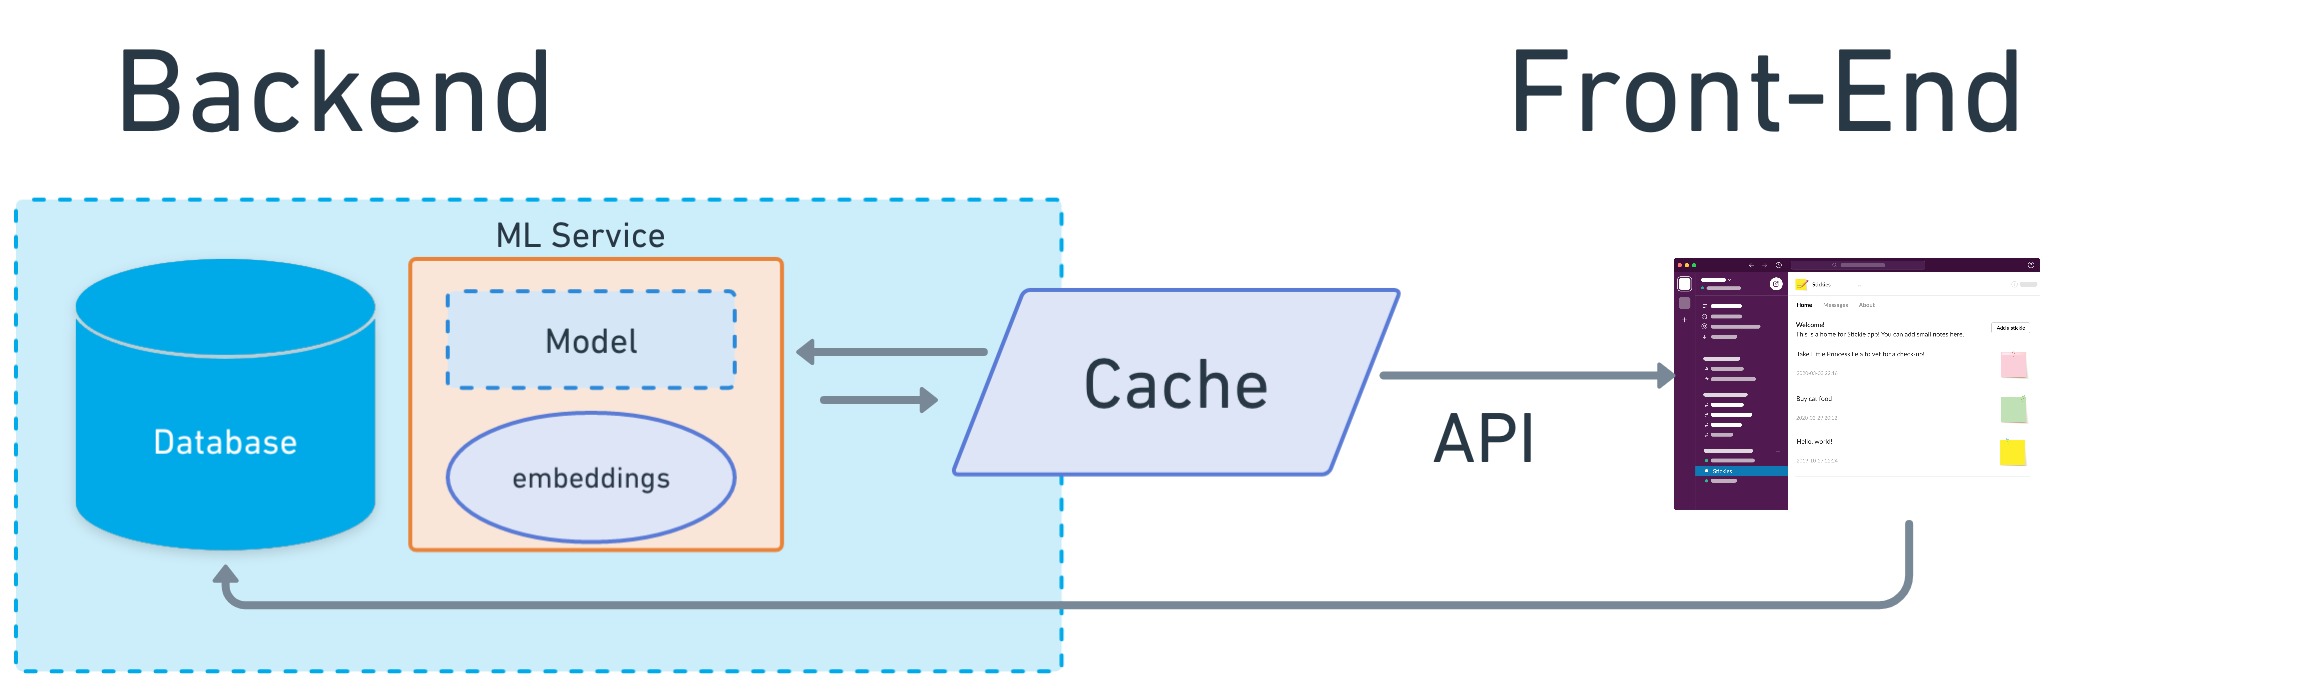
\includegraphics[width=1\textwidth]{figures/web_service_ml.png}
\caption{Embeddings in the context of an application.}
\end{figure}


Engineering systems based on embeddings can be computationally expensive to build and maintain \citep{sharir2020cost}. The need to create, store, and manage embeddings has also recently resulted in the explosion of an entire ecosystem of related products. For example, the recent rise in the development of vector databases to facilitate production-ready use of nearest neighbors semantic queries in machine learning systems\footnote{For a survey of the vector database space today, refer to  \href{https://dmitry-kan.medium.com/landscape-of-vector-databases-d241b279f486}{this article}}, and the rise of embeddings as a service\footnote{Embeddings now are a key differentiator in pricing between \href{https://openai.com/pricing}{on-demand ML services}}.

As such, it's important to understand their context both as end-consumers, product management teams, and as developers who work with them. But in my deep-dive into the embeddings reference material, I found that there are two types of resources: very deeply technical academic papers, for people who are already NLP experts, and surface-level marketing spam blurbs for people looking to buy embeddings-based tech, and that neither of these overlap in what they cover.  

In Systems Thinking, Donella Meadows writes, “You think that because you understand 'one' that you must therefore understand 'two' because one and one make two. But you forget that you must also understand 'and.'" \citep{meadows2008thinking} In order to understand the current state of embedding architectures and be able to decide how to build them, we must understand how they came to be. In building my own understanding, I wanted a resource that was technical enough to be useful enough to ML practitioners, but one that also put embeddings in their correct business and engineering contexts as they become more often used in ML architecture stacks. This is, hopefully, that text.

In this text, we'll examine embeddings from three perspectives, working our way from the highest level view to the most technical. We'll start with the business context, followed by the engineering implementation, and finally look at the machine learning theory, focusing on the nuts and bolts of how they work. On a parallel axis, we'll also travel through time, surveying the earliest approaches and moving towards modern embedding approaches.  

In writing this text, I strove to balance the need to have precise technical and mathematical definitions for concepts and my desire to stay away from explanations that make people's eyes glaze over.  I've defined all technical jargon when it appears for the first time to build context. I include code as a frame of reference for practitioners, but don't go as deep as a code tutorial would\footnote{In other words, I wanted to straddle the "explanation" and "reference" quadrants of \href{https://diataxis.fr/}{the Diátaxis framework }}. So, it would be helpful for the reader to have some familiarity with programming and machine learning basics, particularly after the sections that discuss business context. But, ultimately the goal is to educate anyone who is willing to sit through this, regardless of level of technical understanding.

It's worth also mentioning what this text does not try to be: it does not try to explain the latest advancements in GPT and generative models, it does not try to explain transformers in their entirety, and it does not try to cover all of the exploding field of vector databases and semantic search. I've tried my best to keep it simple and focus on really understanding the core concept of embeddings.

\section{Recommendation as a business problem}

Let's step back and look at the larger context with a concrete example before diving into implementation details.  Let's build a social media network, \textbf{Flutter}, the premier social network for all things with wings. Flutter is a web and mobile app where birds can post short snippets of text, videos, images, and sounds, to let other birds, insects and bats in the area know what’s up. Its business model is based on targeted advertising, and its app architecture includes a "home" feed based on birds that you follow, made up of small pieces of multimedia content called \textbf{“flits”}, which can be either text, videos, or photos. The home feed itself is by default in reverse chronological order that is curated by the user. But we also would like to offer personalized, recommended flits so that the user finds interesting content on our platform that they might have not known about before.  

\begin{figure}[H]
\centering
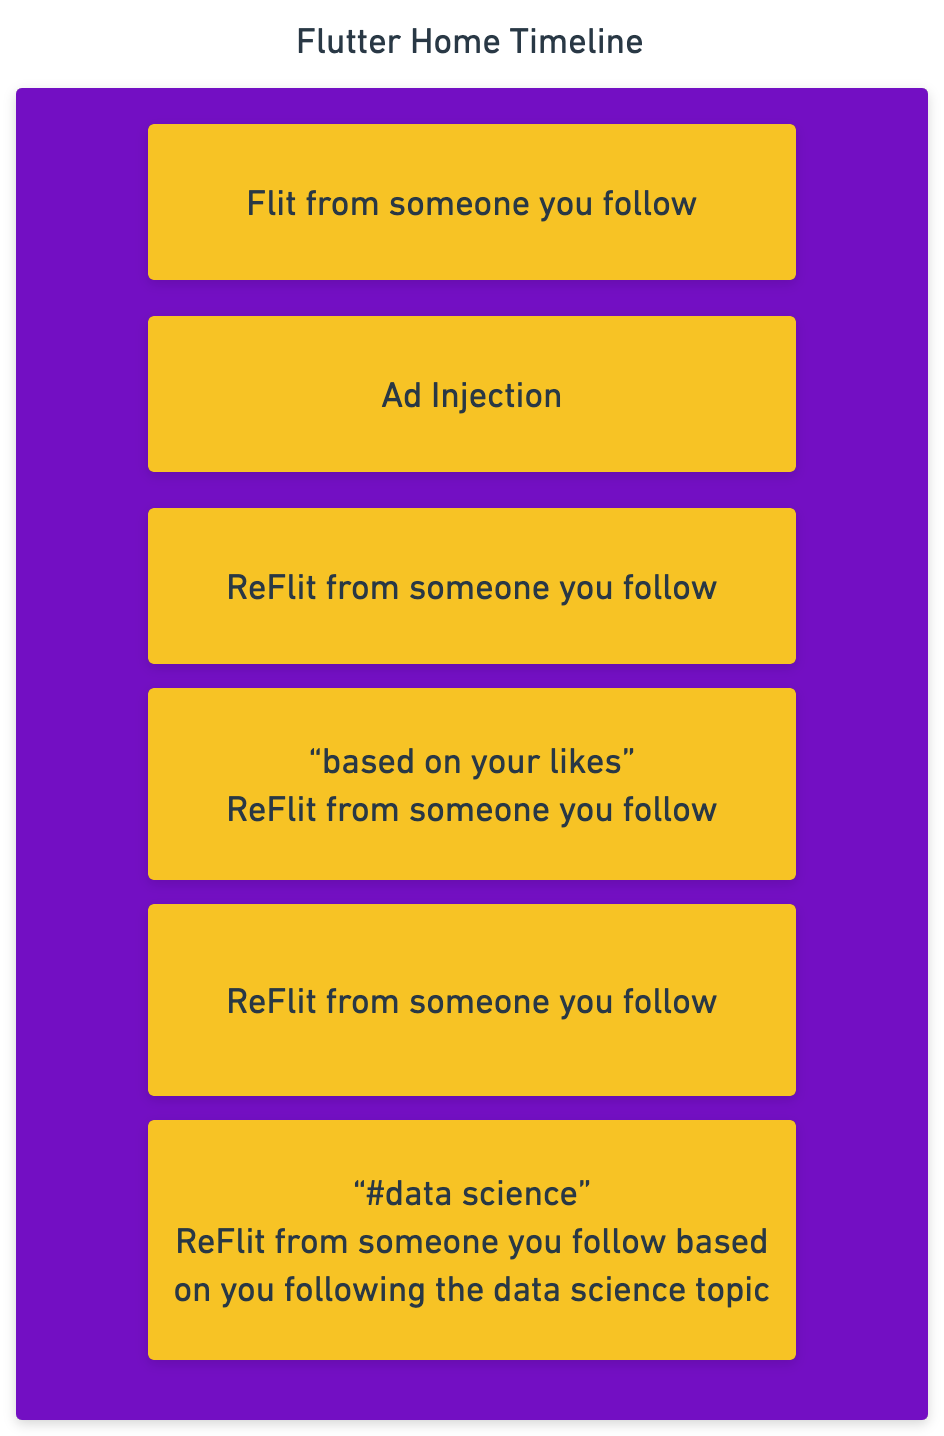
\includegraphics[width=.5\textwidth]{figures/timeline.png}
\caption{Flutter's content timeline in a social feed with a blend of organic followed content, advertising, and recommendations.}
\end{figure}

How do we solve the problem of what to show in the timeline here so that our users find the content relevant and interesting, and balance the needs of our advertisers and business partners?

In many cases, we can approach engineering solutions without involving machine learning. In fact, we should definitely start without it \citep{zinkevich2017rules} because machine learning adds a tremendous amount of complexity to our working application \citep{sculley2014machine}. In the case of the Flutter home feed, though, machine learning forms a business-critical function part of the product offering. From the business product perspective, the objective is to offer Flutter’s users content that is relevant\footnote{The specific definition of a relevant item in the recommendations space varies and is under intense academic and industry debate, but generally it means an item that is of interest to the user}, interesting, and novel so they continue to use the platform.  If we do not build discovery and personalization into our content-centric product, Flutter users will not be able to discover more content to consume and will disengage from the platform.

This is the case for many content-based businesses, all of which have feed-like surface areas for recommendations, including Netflix, Pinterest, Spotify, and Reddit.  It also covers e-commerce platforms, which must surface relevant items to the user, and information retrieval platforms like search engines, which must provide relevant answers to users upon keyword queries. There is a new category of hybrid applications involving question-and-answering in semantic search contexts that is arising as a result of work around the GPT series of models, but for the sake of simplicity, and because that landscape changes every week, we'll stick to understanding the fundamental underlying concepts.

In subscription-based platforms\footnote{In ad-based services, the line between retention and revenue is a bit murkier, and we have often what's known as a multi-stakeholder problem, where the actual optimized function is a balance between meeting the needs of the user and meeting the needs of the advertiser \citep{zheng2017multi}.  In real life, this can often result in a process of enshittifcation \citep{doctorow_2023} of the platform that leads to extremely suboptimal end-user experiences. So, when we create Flutter, we have to be very careful to balance these concerns, and we'll also assume for the sake of simplification that Flutter is a Good service that loves us as users and wants us to be happy.}, there is clear business objective that's tied directly to the bottom line, as outlined in this 2015 paper  \citep{steck2021deep}  about Netflix's recsys:

\begin{quote}

The main task of our recommender system at Netflix is to help our members discover content that they will watch and enjoy to maximize their long-term satisfaction. This is a challenging problem for many reasons, including that every person is unique, has a multitude of interests that can vary in different contexts, and needs a recommender system most when they are not sure what they want to watch. Doing this well means that each member gets a unique experience that allows them to get the most out of Netflix. As a monthly subscription service, member satisfaction is tightly coupled to a person’s likelihood to retain with our service, which directly impacts our revenue.
\end{quote}

Knowing this business context, and given that personalized content is more relevant and generally gets higher rates of engagement \citep{jannach2010recommender} than non-personalized forms of recommendation on online platforms,\footnote{For more, see  \href{http://www.recommenderbook.net/media/Recommender_Systems_An_Introduction_Chapter08_Case_study.pdf}{this case study} on personalized recommendations as well as \href{https://www.arxiv-vanity.com/papers/1906.03109/}{the intro section of this paper} which covers many personalization use-cases.}  how and why might we use embeddings in machine learning workflows in Flutter to show users flits that are interesting to them personally? We need to first understand how web apps work and where embeddings fit into them.

\subsection{Building a web app}

 Most of the apps we use today --- Spotify, Gmail, Reddit, Slack, and Flutter --- are all designed based on the same foundational software engineering patterns. They are all apps available on web and mobile clients. They all have a front-end where the user interacts with the various \textbf{product features} of the applications, an API that connects the front-end to back-end elements, and a database that processes data and remembers state.
 
 \begin{formal}
 As an important note, \textbf{features} have many different definitions in machine learning and engineering. In this specific case, we mean collections of code that make up some front-end element, such as a button or a panel of recommendations. We'll refer to these as \textbf{product features}, in contrast with \textbf{machine learning features}, which are input data into machine learning models.
  \end{formal}
 
 This application architecture is commonly known as \textbf{model-view-controller} pattern  \citep{fowler2012patterns}, or in common industry lingo, a \textbf{CRUD} app, named for the basic operations that its API allows to manage application state: create, read, update, and delete.
 
\begin{figure}[H]
\centering
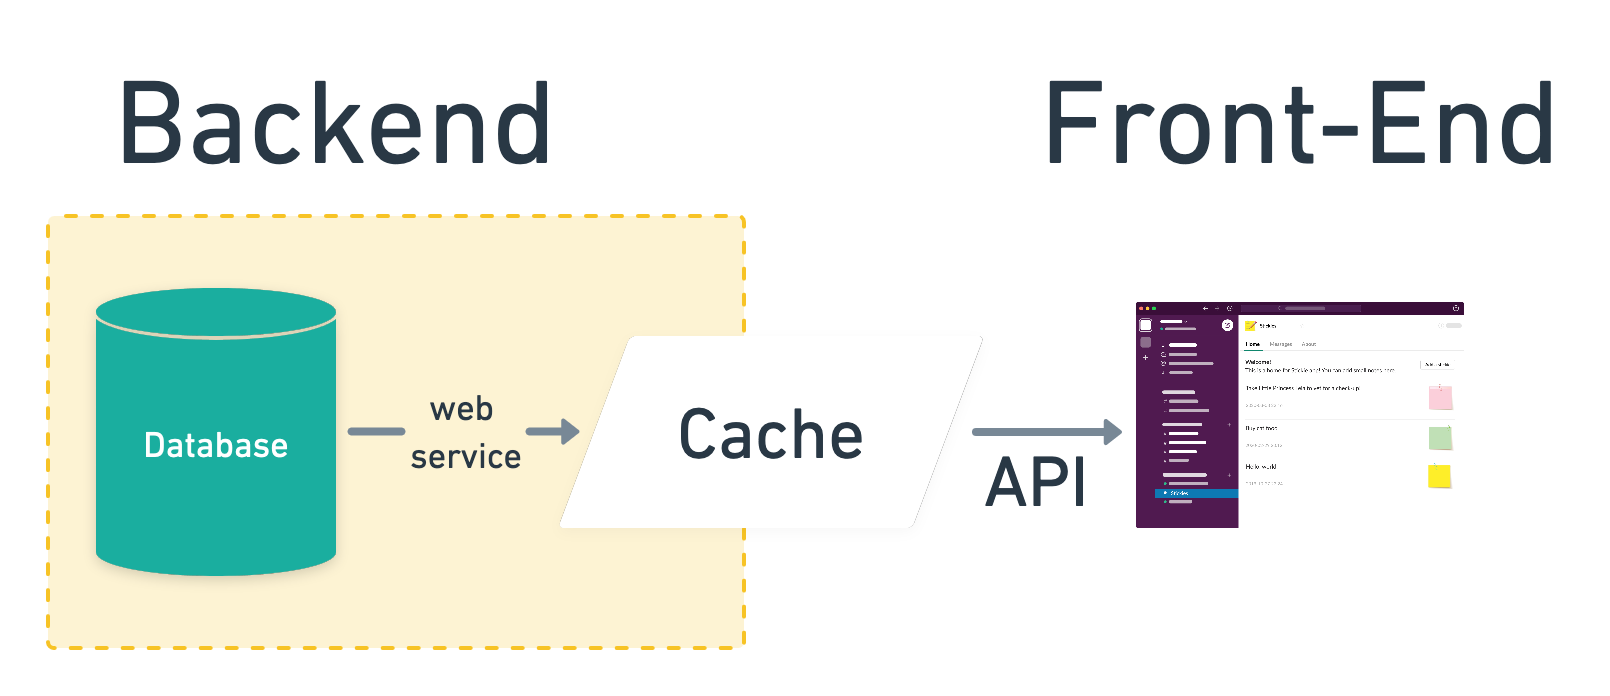
\includegraphics[width=.9\textwidth]{figures/web_service.png}
\caption{Typical CRUD web app architecture}
\end{figure}

When we think of structural components in the architectures of these applications, we might think first in terms of product features. In an application like Slack, for example, we have the ability to post and read messages, manage notifications, and add custom emojis. Each of these can be seen as an application feature. In order to create features, we have to combine common elements like databases, caches, and web services. All of this happens as the client talks to the API, which talks to the database to process data. At a more granular, program-specific level, we might think of foundational data structures like arrays or hash maps, and lower still, we might think about memory management and network topologies. These are all foundational elements of modern programming.

At the feature level, though, we see that it not only includes the typical CRUD operations, such as the ability to post and read Slack messages, but also elements that are more than operations that alter database state. Some features such as \href{https://slack.engineering/personalized-channel-recommendations-in-slack/}{personalized channel suggestions}, \href{https://slack.engineering/search-at-slack/}{returning relevant results through search queries}, and \href{https://slack.engineering/email-classification/}{predicting Slack connection invites} necessitates the use of  machine learning.

\begin{figure}[H]
\centering
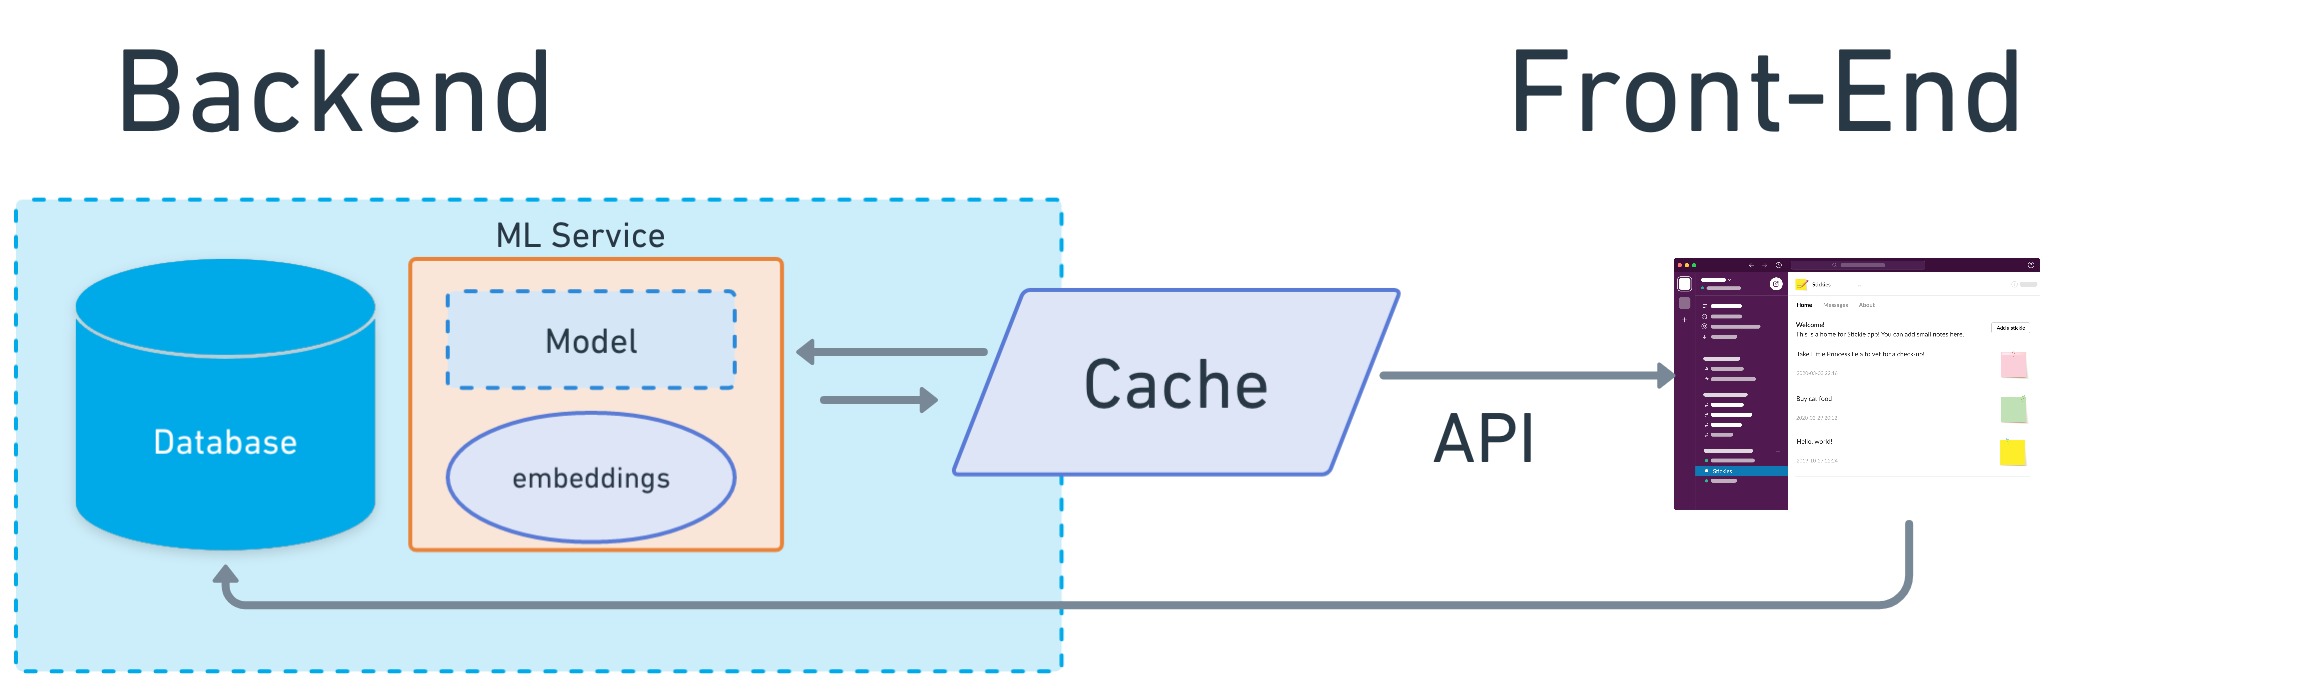
\includegraphics[width=\textwidth]{figures/web_service_ml.png}
\caption{CRUD App with Machine learning service}
\end{figure}

\subsection{Rules-based systems versus machine learning}

To understand where embeddings fit into these systems, it first  makes sense to understand where machine learning fits in at Flutter, or any given company, as a whole. In a typical consumer company, the user-facing app is made up of product features written in code, typically written as services or parts of services. To add a new web app feature, we write code based on a set of business logic requirements. This code acts on data in the app to develop our new feature.


In a  typical data-centric software development lifecycle, we start with the business logic. For example, let's take the ability to post messages. We'd like users to be able to input text and emojis in their language of choice, have the messages sorted chronologically, and render correctly on web and mobile. These are the business requirements. We use the input data, in this case, user messages, and format them correctly and sort chronologically, at low latency, in the UI.

\begin{figure}[H]
\centering
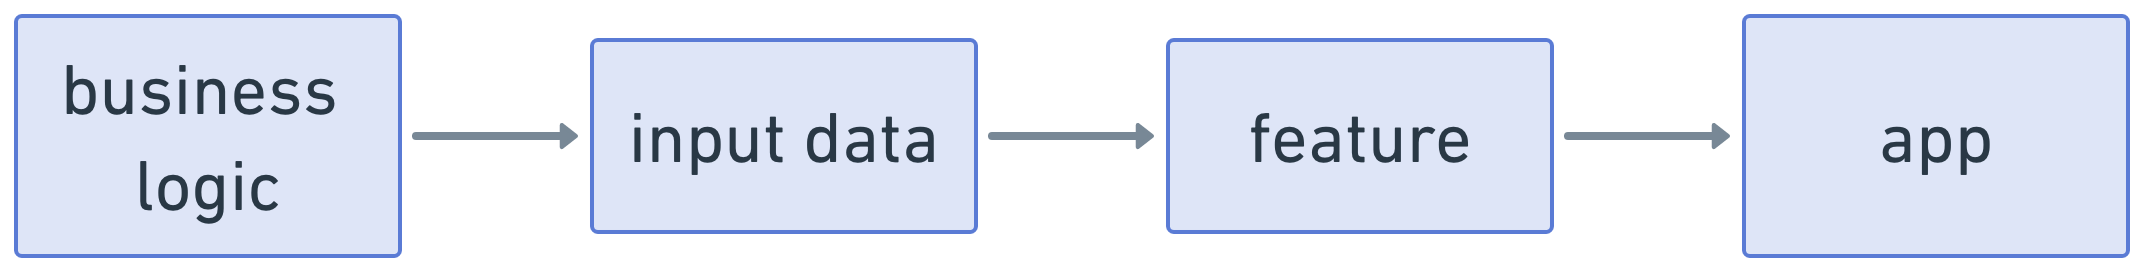
\includegraphics[width=.75\textwidth]{figures/app_flow.png}
\caption{A typical application development lifecycle}
\end{figure}

Machine learning-based systems are typically also services in the backend of web applications. They are integrated into production workflows. But, they process data much differently. In these systems, we don't start with business logic. We start with input data that we use to build a model that will suggest the business logic for us. For more on the specifics of how to think about these data-centric engineering systems, see Kleppmann\cite{kleppmann2017designing}.

This requires thinking about application development slightly differently, and when we write an application that includes machine learning models as input, however, we’re inverting the traditional app lifecycle. What we have instead, is data plus our desired outcome. The data is combined into a model, and it is this model which instead generates our business logic that builds features.

\begin{figure}[H]
\centering
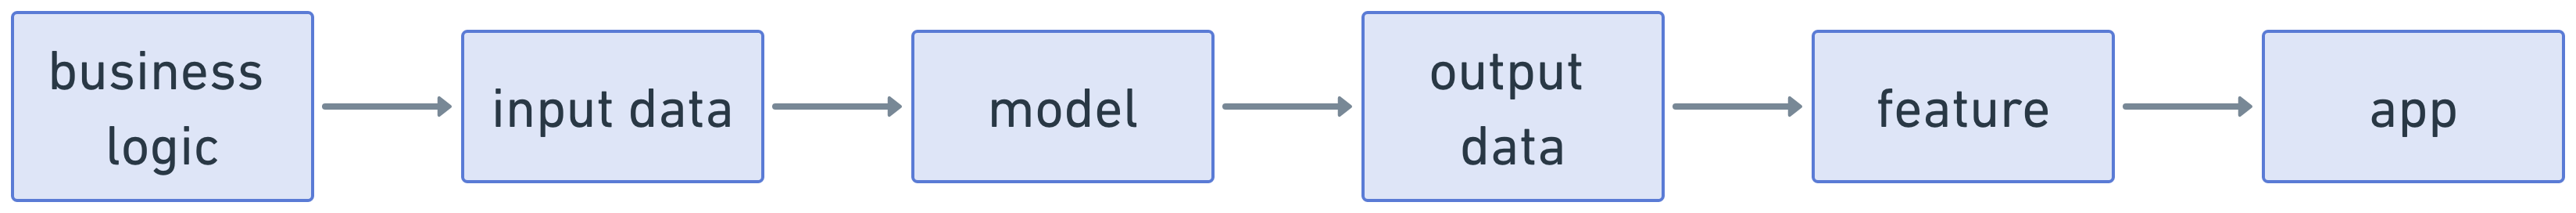
\includegraphics[width=.95\textwidth]{figures/ml-flow.png}
\caption{ML Development lifecycle}
\end{figure}

In short, the difference between programming and machine learning development is that we are not generating answers through business rules, but business rules through data. These rules are then re-incorporated into the application.

\begin{figure}[H]
\centering
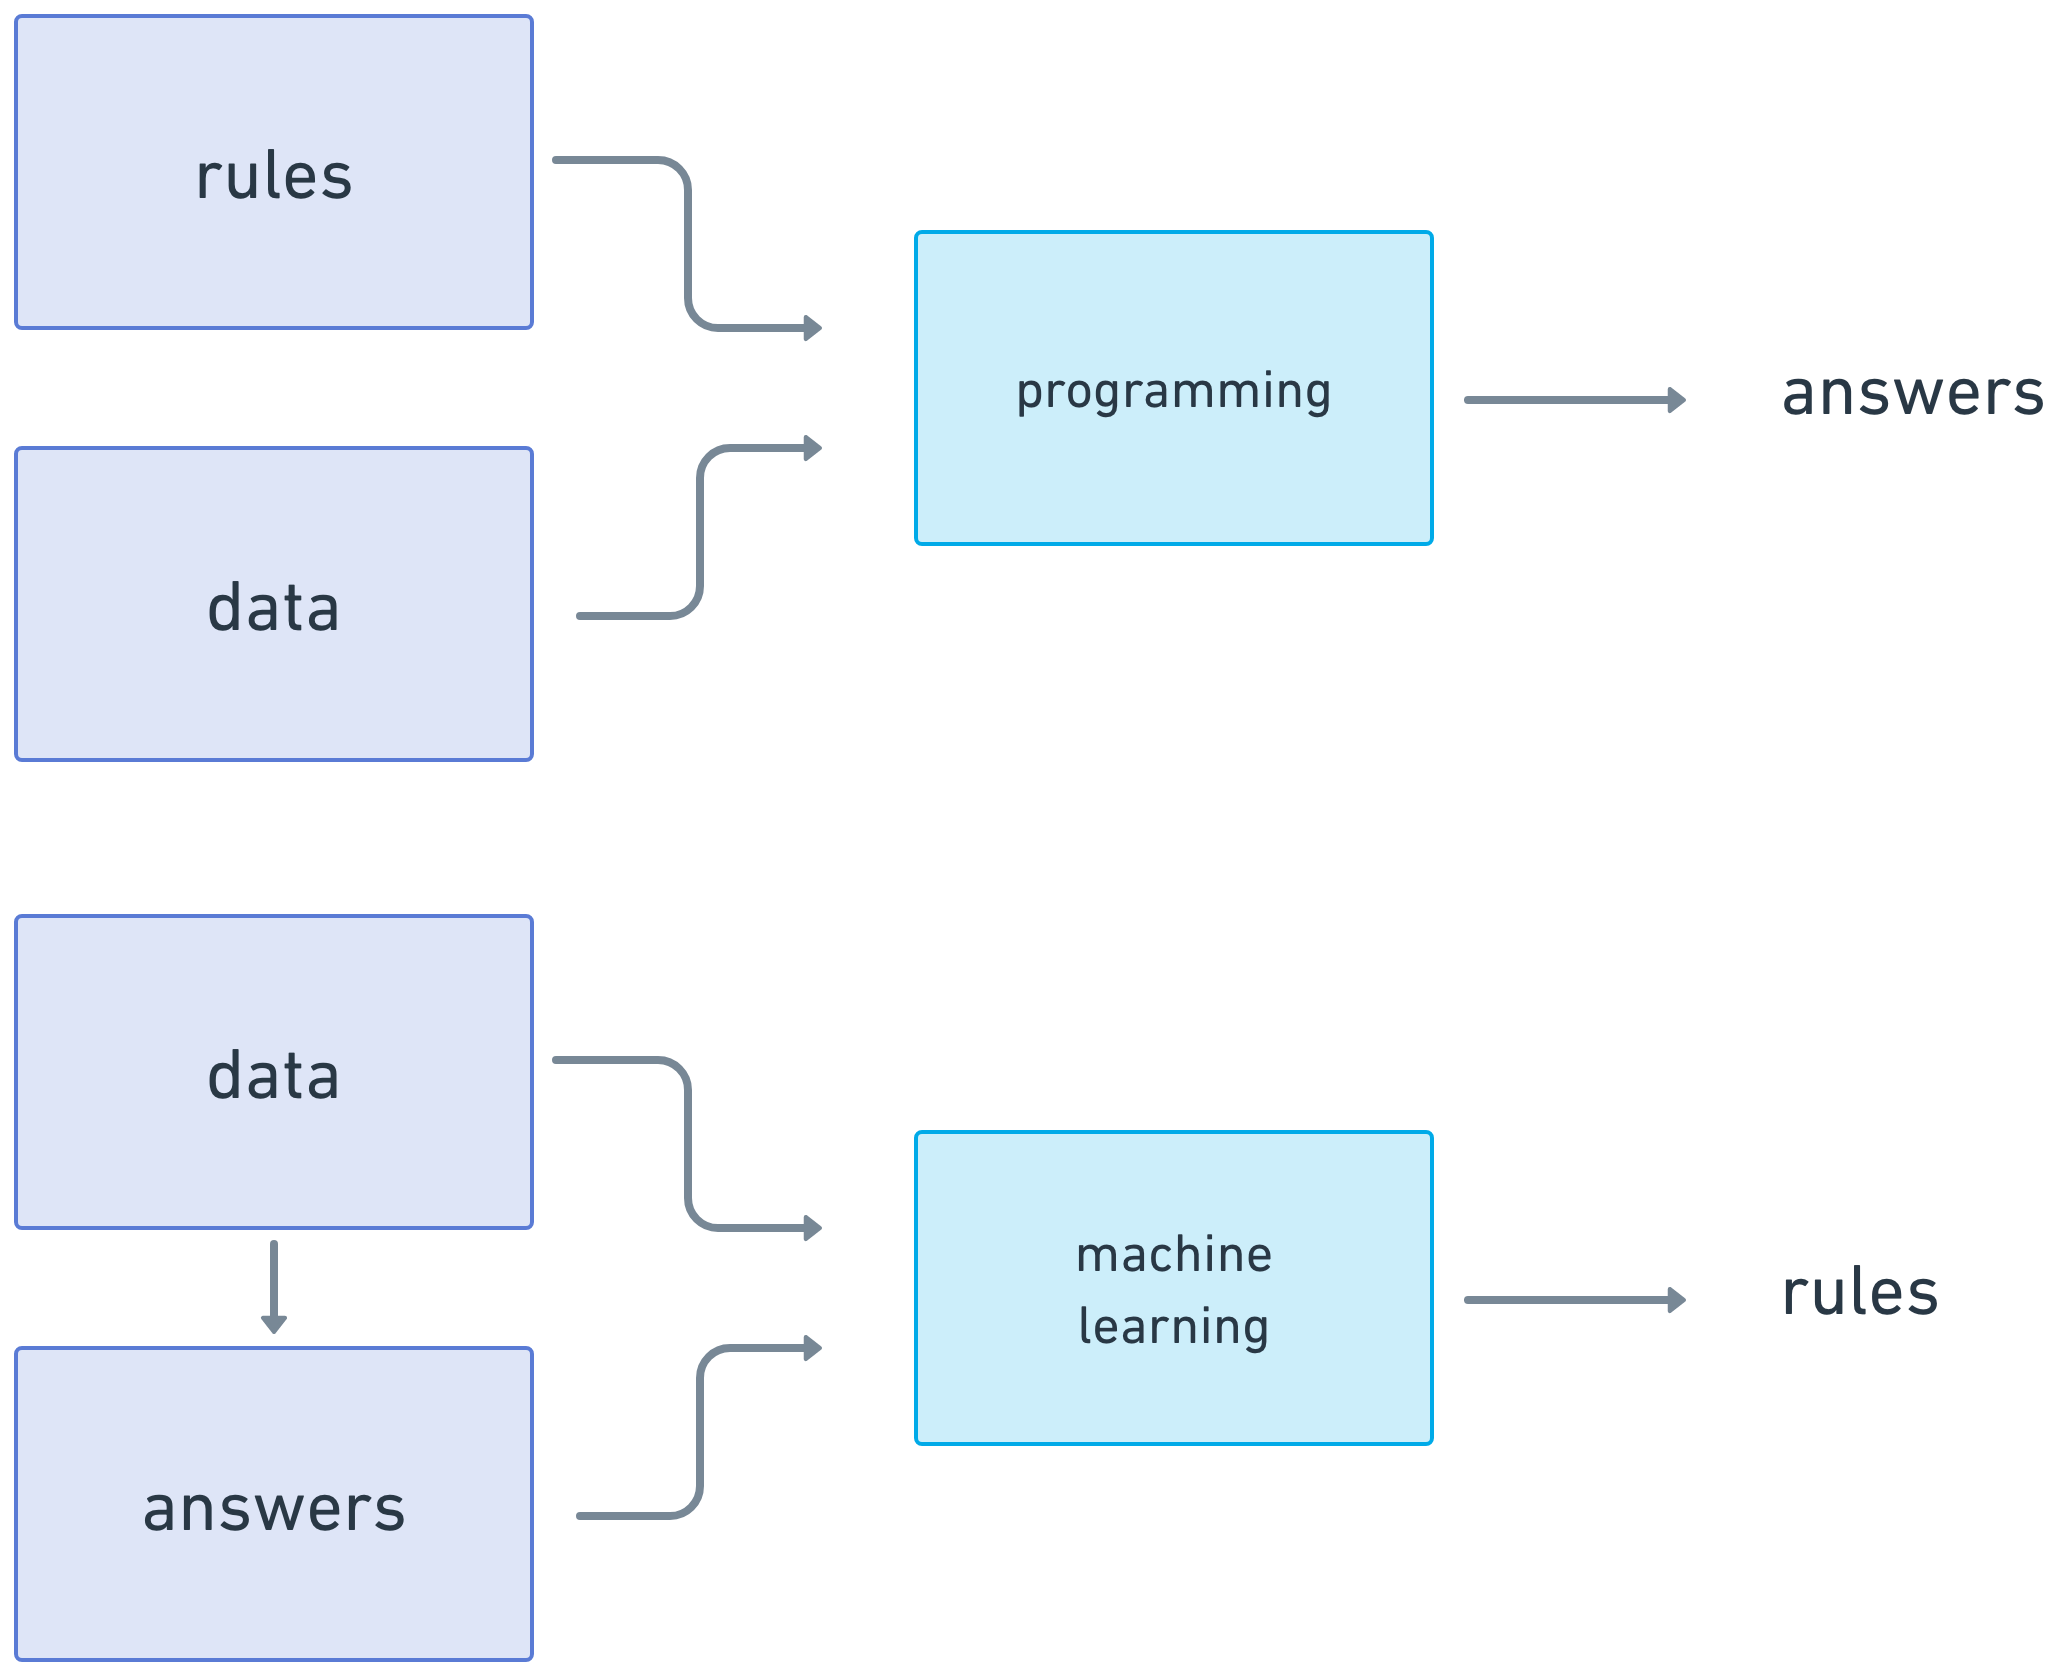
\includegraphics[width=.75\textwidth]{figures/rules_ml.png}
\caption{Generating answers via machine learning. The top chart shows a classical programming approach with rules and data as inputs, while the bottom chart shows a machine learning approach with data and answers as inputs.  \citep{chollet2021deep}}
\end{figure}

As an example, with Slack, for the channel recommendations product feature, we are not hard-coding a list of channels that need to be called from the organization's API. We are feeding in data about the organization's users (what other channels they've joined, how long they've been users, what channels the people they've interacted the most with Slack in), and building a model on that data that recommends a non-deterministic, personalized list of channels for each user that we then surface through the UI.

\begin{figure}[H]
\centering
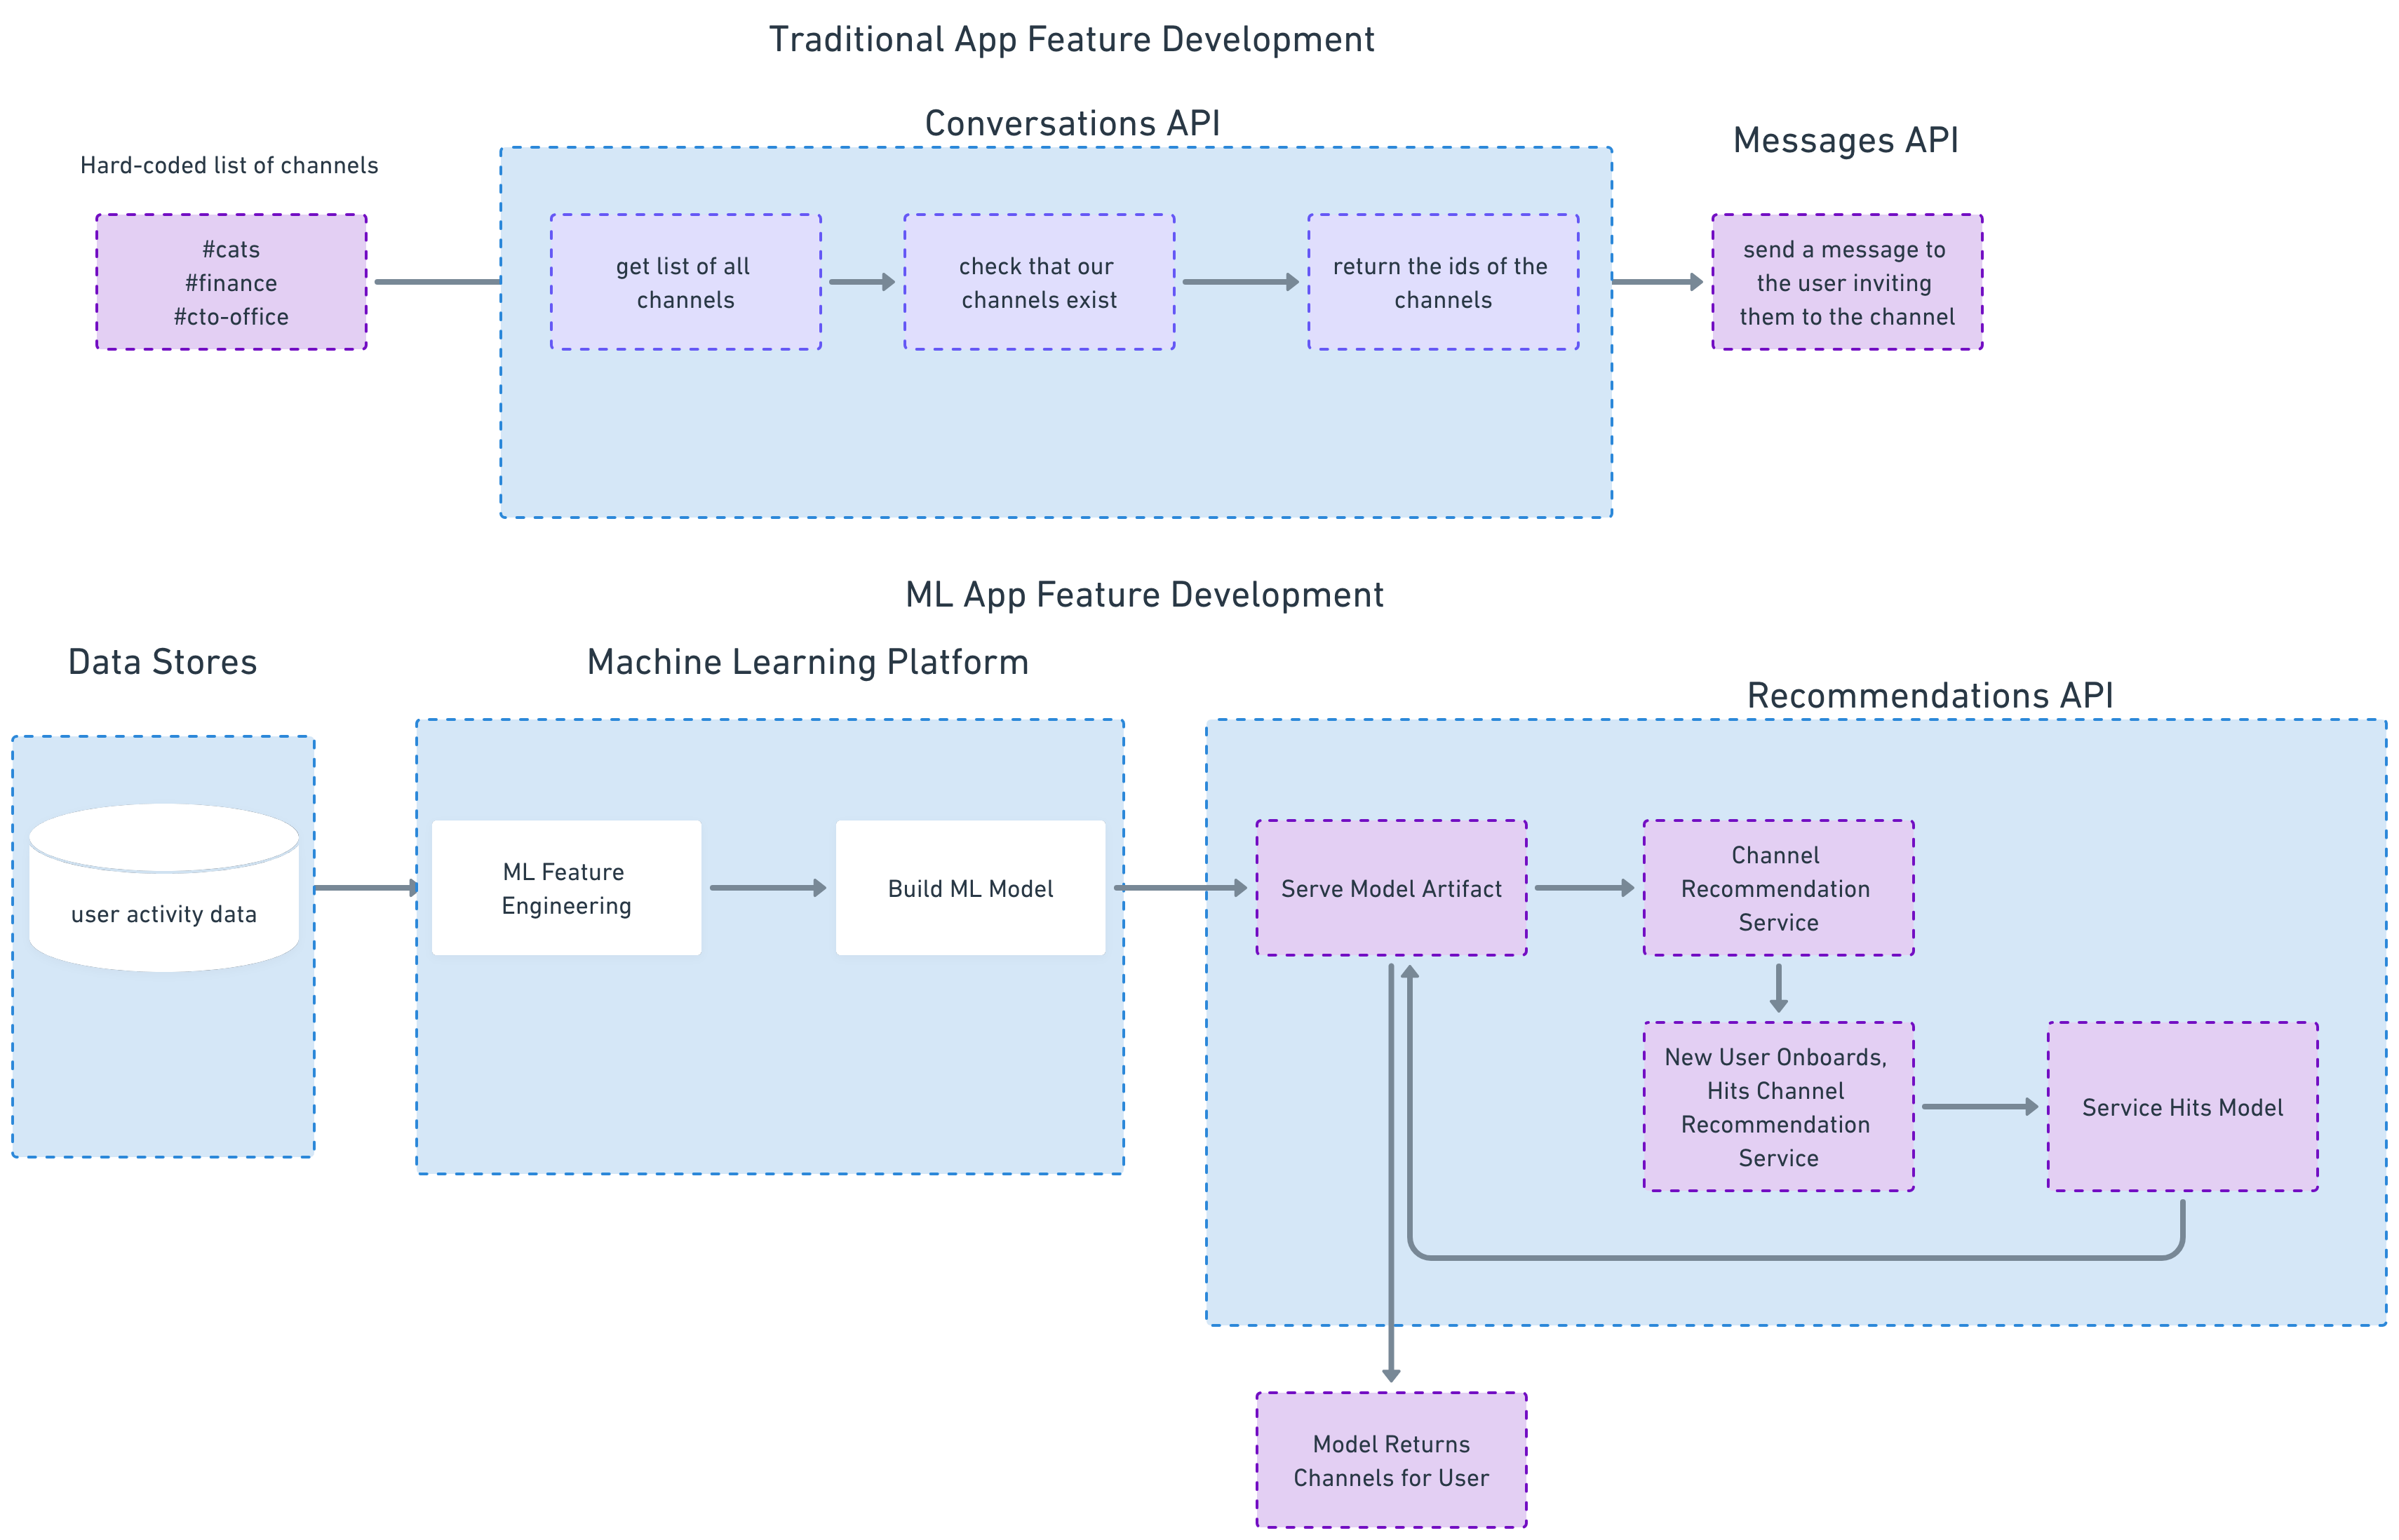
\includegraphics[width=.95\textwidth]{figures/mlnotml.png}
\caption{Traditional versus ML architecture and infra}
\end{figure}

\subsection{Building a web app with machine learning}

All machine learning systems can be examined through how they accomplish these four steps. When we build models, our key questions should be, "what kind of input do we have and how is it formatted", and "what do we get as a result." We'll be asking this for each of the approaches we look at.  When we build a machine learning system, we start by processing data and finish by serving a learned model artifact.

The four components of a machine learning system are\footnote{There are infinitely many layers of horror in ML systems \citep{kreuzberger2022machine}. These are still the foundational components.}:

\begin{formal}
\begin{itemize}
  \item \textbf{Input data} - processing data from a database or streaming from a production application for use in modeling
  \item \textbf{Feature Engineering and Selection} - The process of examining the data and cleaning it to pick features. In this case, we mean features as attributes of any given element that we use as inputs into machine learning. Examples of features are: user name, geographic location, how many times they've clicked on a button for the past 5 days, and revenue. This piece always takes the longest in any given machine learning system, and is also known as finding \textbf{representations} \citep{bengio2013representation} of the data that best fit the machine learning algorithm. This is where, in the new model architectures, we use embeddings as input.
  \item \textbf{Model Building} - We select the features that are important and train our model, iterating on different performance metrics over and over again until we have an acceptable model we can use. Embeddings are also the output of this step that we can use in other, downstream steps.
  \item \textbf{Model Serving} - Now that we have a model we like, we serve it to production, where it hits a web service, potentially cache, and our API where it then propagates to the front-end for the user to consume as part of our web app
\end{itemize}
\end{formal}

\begin{figure}[H]
\centering
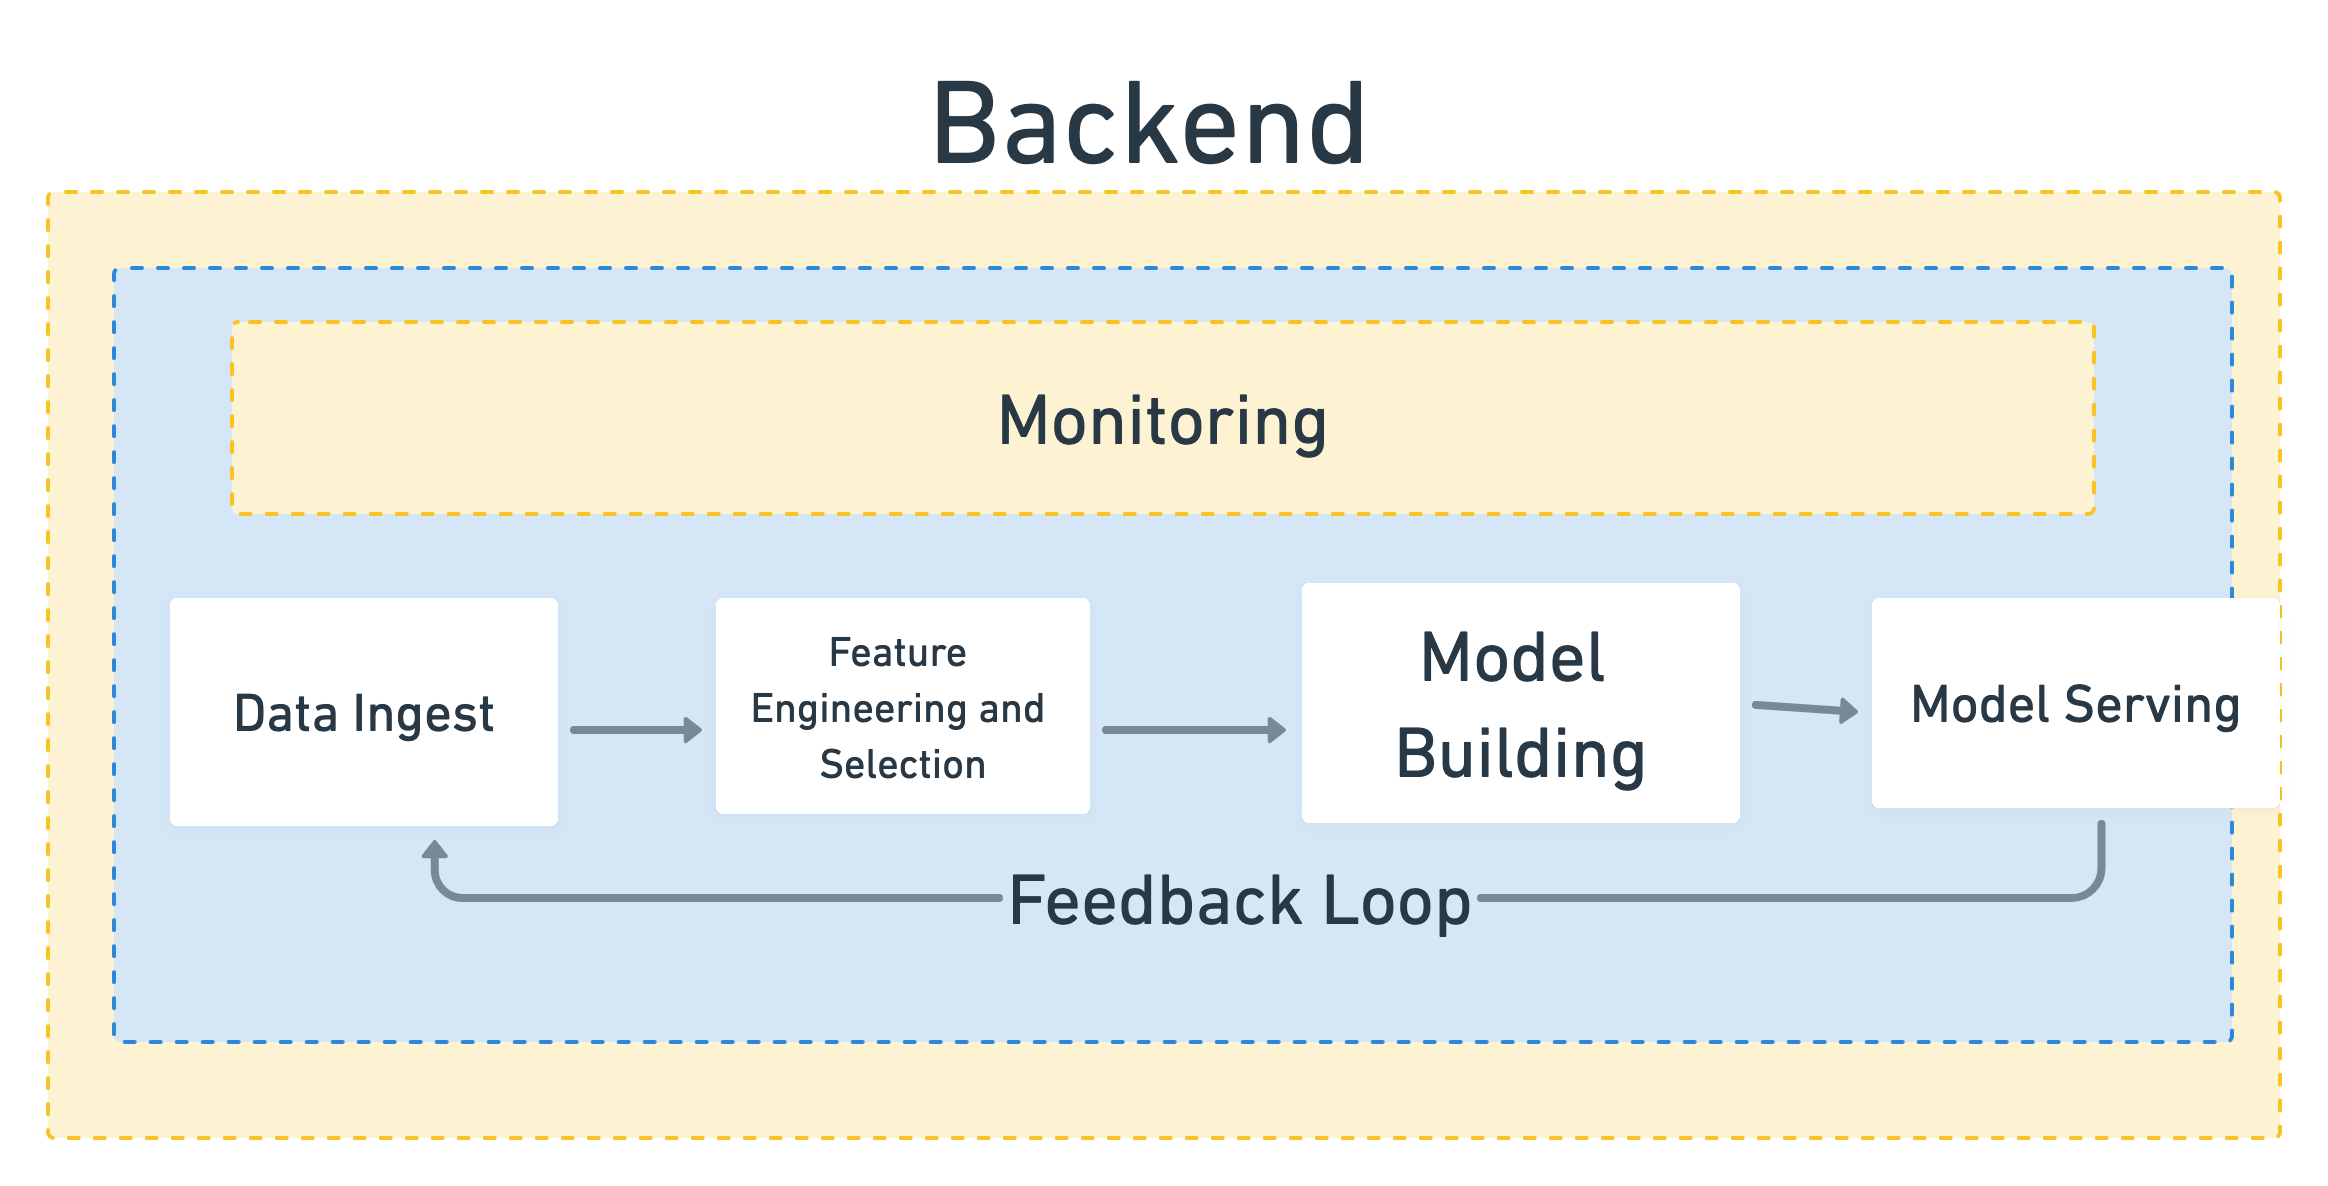
\includegraphics[width=1\textwidth]{figures/ml_system.png}
\caption{CRUD app with ML}
\end{figure}

Within machine learning, there are many approaches we can use to fit different tasks.  Machine learning workflows that are most effective are formulated as solutions to both a specific business need and a machine learning \textbf{task}. Tasks can best be thought of as approaches to modeling within the categorized solution space. For example, learning a regression model is a specific case of a task. Others include clustering, machine translation, anomaly detection, similarity matching, or semantic search.  The  three highest-level types of ML tasks are  \textbf{supervised}, where we have training data that can tell us whether the results the model predicted are correct according to some model of the world. The second is \textbf{unsupervised}, where there is not a single ground-truth answer. An example here is clustering of our customer base. A clustering model can detect patterns in your data but won't explicitly label what those patterns are. The third is \textbf{reinforcement learning}  which is separate from these two categories and formulated as a game theory problem: we have an agent moving through an environment and we'd like to understand how to optimally move them through a given environment using explore-exploit techniques. We'll focus on supervised learning, with a look at unsupervised learning with PCA and Word2Vec.
 
\begin{figure}[H]
    \centering
    \resizebox{.8\textwidth}{!}{%
\begin{forest}
  for tree={
    align=center,
    parent anchor=south,
    child anchor=north,
    font=\sffamily,
    edge={->,thick},
    l sep+=20pt,
  }
[Machine Learning
[Supervised Machine Learning
[SVM]
[Regression]
[{Neural\\Networks}]
]
[{Unsupervised\\Machine\\Learning}, align=center
[Clustering]
[Dimensionality\\Reduction
[PCA]
]
]
[{Reinforcement\\Learning}]
]
\end{forest}}
	 \caption{Machine learning task solution space and model families}
\end{figure}


\subsection{Formulating a machine learning problem}

As we saw in the last section, machine learning is a process that takes data as input to produce rules for how we should classify something or filter it or recommend it, depending on the task at hand. In any of these cases, for example, to generate a set of potential candidates, we need to construct a \textbf{model}.

A machine learning model is a set of instructions for generating a given output from data. The instructions are learned from the features of the input data itself.   For Flutter, an example of a model we'd like to build is a \textbf{candidate generator} that picks flits similar to flits our birds have already liked, because we think users will like those, too. For the sake of building up the intuition for a machine learning workflow, let's pick a super-simple example that is not related to our business problem, linear regression, which gives us a continuous variable as output in response.

For example, let's say, given the number of posts a user has made and how many posts they've liked, we'd like to predict how many days they're likely to continue to stay on Flutter.  For traditional \textbf{supervised} modeling approaches using tabular data, we start with our input data, or a \textbf{corpus} as it's generally known in machine learning problems that deal with text in the field known as \textbf{NLP} (natural language processing).

We're not doing NLP yet, though, so our input data may look something like this, where we have a UID (userid) and some attributes of that user, such as the number of times they've posted and number of posts they've liked. These are our machine learning \textbf{features}.

\begin{table}[H]
  \centering
    \caption{Tabular Input Data for Flutter Users}
\begin{tabular}{|l|l|l|l|}
\hline
\rowcolor[HTML]{D5E7F7}
bird\_id & bird\_posts & bird\_likes \\ \hline
012 	 & 2  		   	 & 5  		 \\ \hline
013 	 & 0  		   	 & 4  		 \\ \hline
056 	 & 57 		   	 & 70 		 \\ \hline
612 	 & 0  				 & 120		 \\ \hline
\end{tabular}
\end{table}

We'll need part of this data to train our model, part of it to test the accuracy of the model we've trained, and part to tune meta-aspects of our model. These are known as \textbf{hyperparameters}.

We take two parts of this data as holdout data that we don't feed into the model. The first part, the \textbf{test set}, we use to validate the final model on data it's never seen before. We use the second split, called the \textbf{validation set}, to check our hyperparameters  during the model training phase. In the case of linear regression, there are no true hyperparameters, but we'll need to keep  in mind that we will need to tune the model's metadata for more complicated models.

Let's assume we have 100 of these values.  A usual accepted split is to use 80\% of data for training and 20\% for testing. The reasoning is we want our model to have access to as much data as possible so it learns a more accurate representation.

In general, our goal is to feed our input into the model, through a function that we pick, and get some predicted output, $f(X) \rightarrow y$.

\begin{figure}[H]
  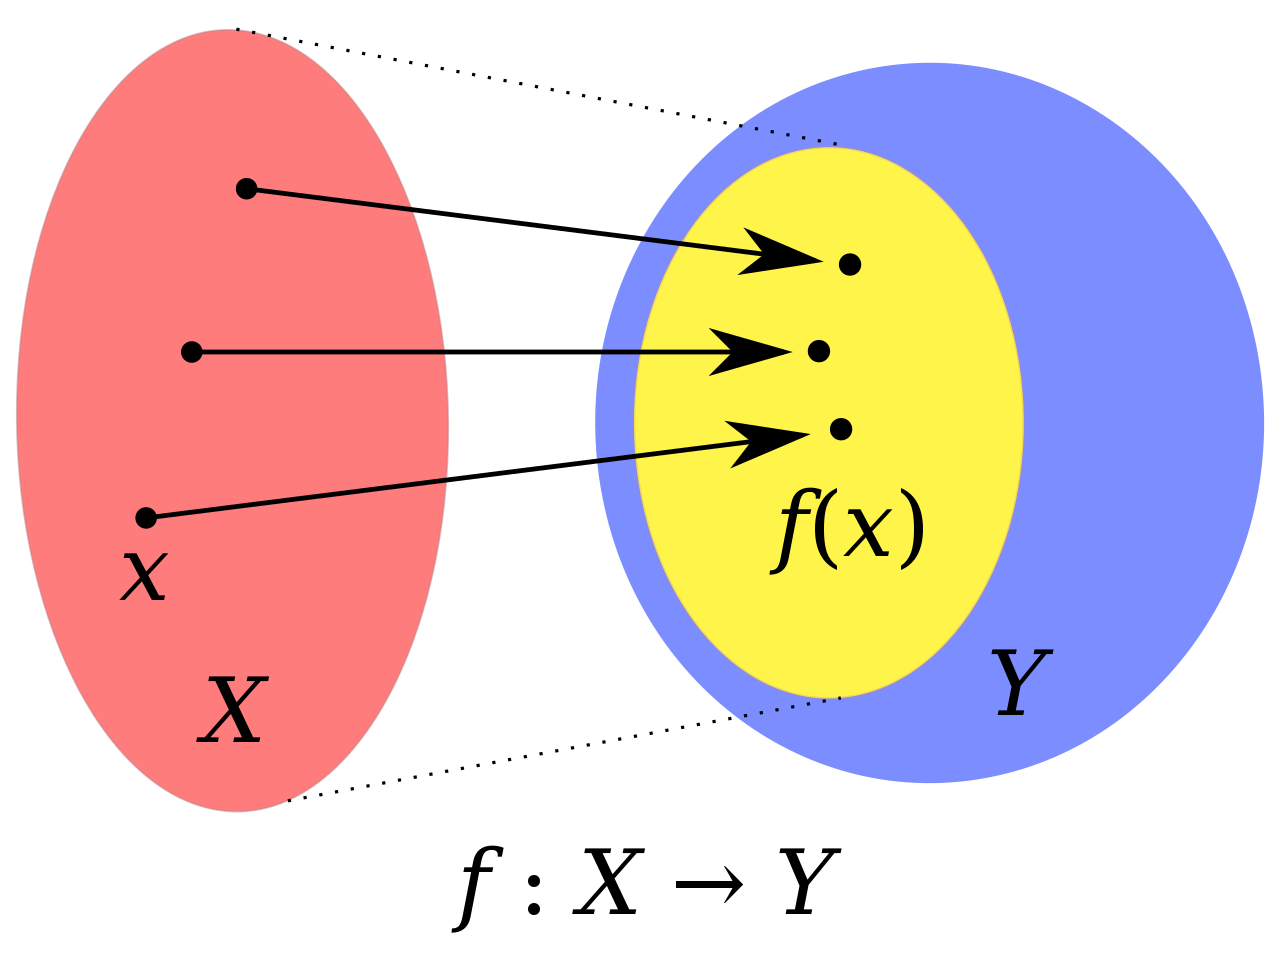
\includegraphics[width=.8\linewidth]{figures/function.png}
  \caption{How inputs map to outputs in ML functions  \citep{klein2013coding}}
\end{figure}

For our simple dataset, we can use the linear regression equation:

\begin{equation}
y = x_1\beta_1 + x_2\beta_2 + \varepsilon
\end{equation}

This tells us that the output, $y$, can be predicted by two input variables, $x_1$ (bird posts) and $x_2$ (bird likes) with their given weights, $\beta_1$ and $\beta_2$, plus an error term $\varepsilon$, or the distance between each data point and the regression line generated by the equation. Our task is to find the smallest sum of squared differences between each point and the line, in other words to minimize the error, because it will mean that, at each point, our predicted y is as close to our actual y as we can get it, given the other points.

\begin{equation}
y = x_1\beta_1 + x_2\beta_2 + \varepsilon
\end{equation}

The heart of machine learning is this training phase, which is the process of finding a combination of model instructions and data that accurately represent our real data, which, in supervised learning, we can validate by checking the correct "answers" from the test set.

\begin{figure}[H]
  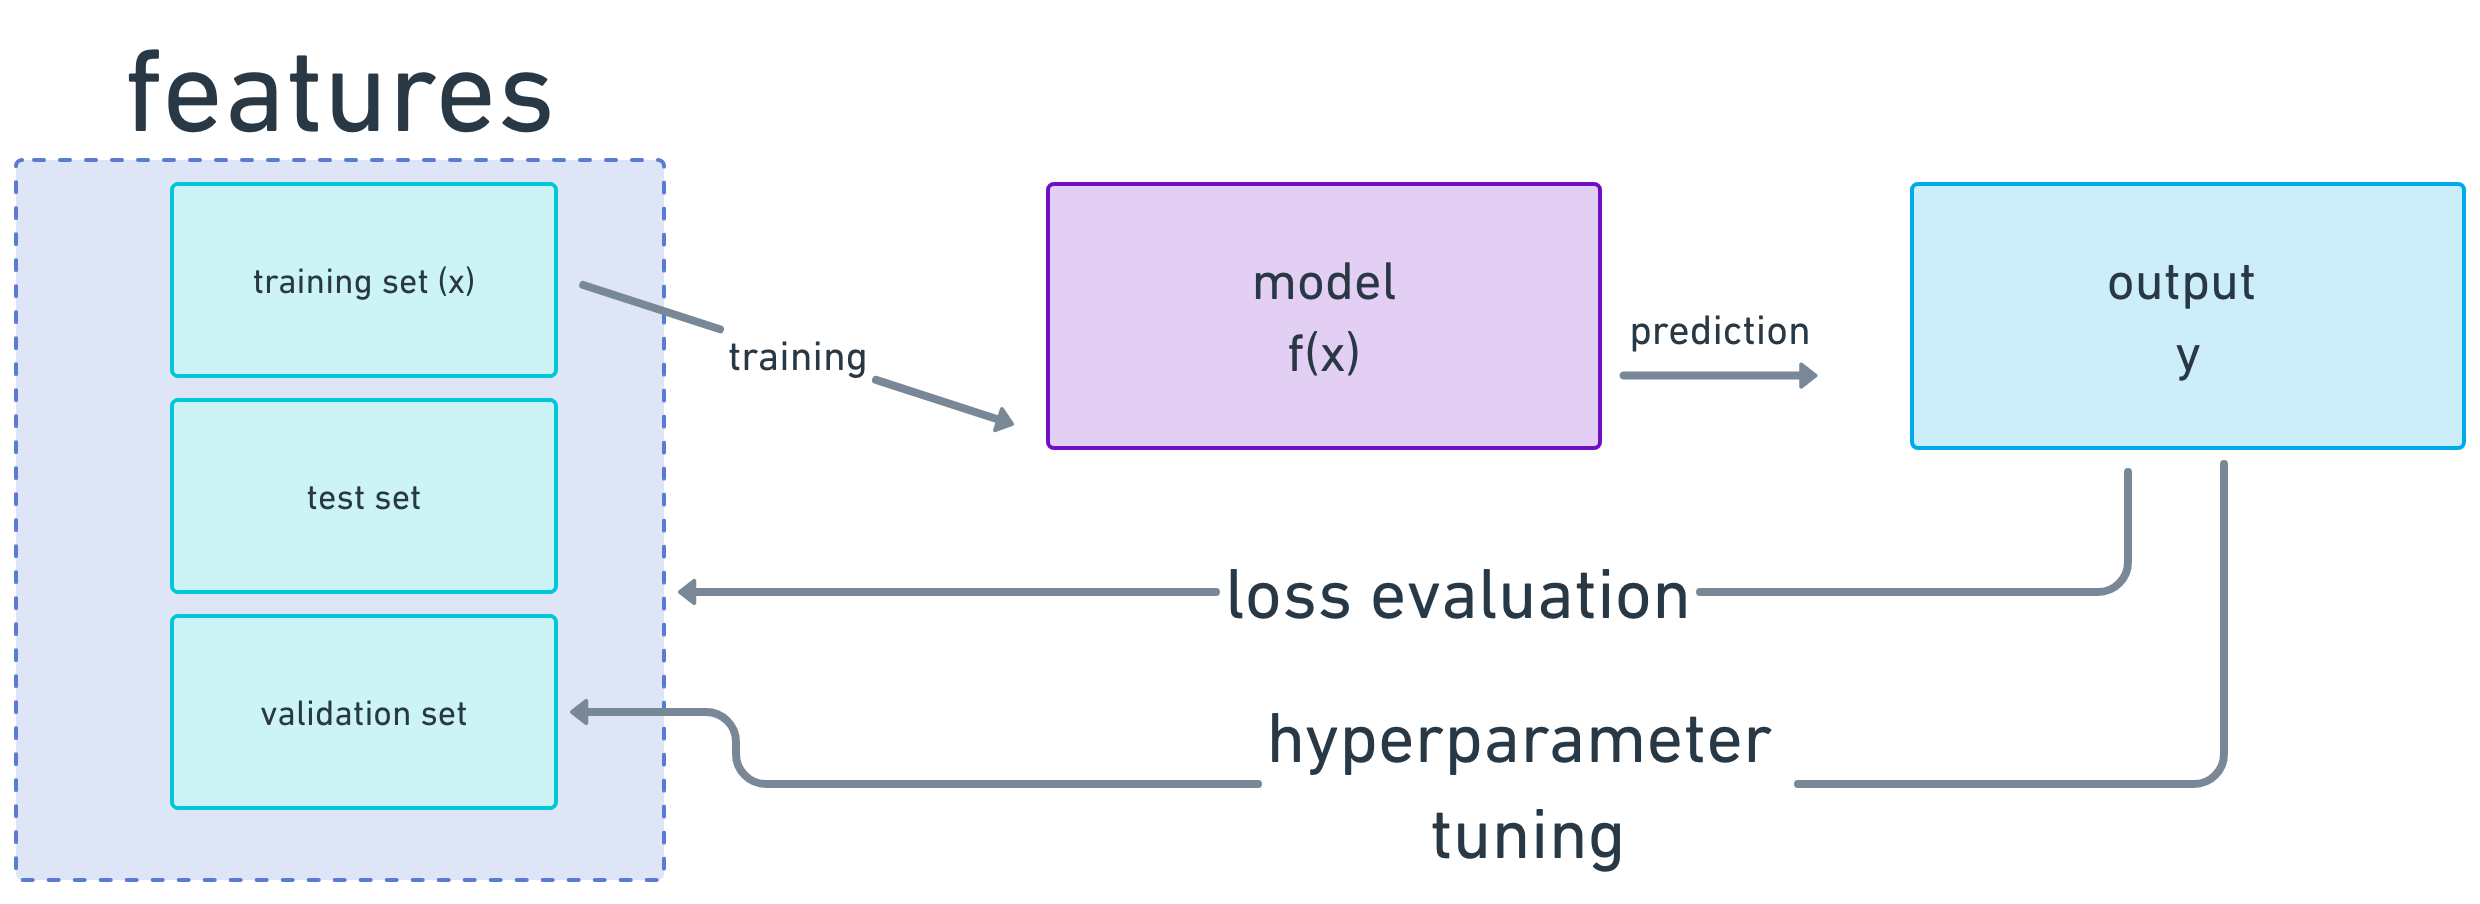
\includegraphics[width=\linewidth]{figures/model_cycle.png}
  \caption{The cycle of machine learning model development}
\end{figure}

As the first round of training starts, we have our data. We \textbf{train} --- or build  --- our model by initializing it with a set of inputs, $X$. These are from the training data. $\beta_1$ and $\beta_2$ are either initialized by setting to zero or initialized randomly (depending on the model, different approaches work best), and we calculate $\hat{y}$, our predicted value for the model. $\epsilon$ is derived from the data and the estimated coefficients once we get an output.

\begin{equation}
y = 2\beta_1 + 5\beta_2 + \varepsilon
\end{equation}

How do we know our model is good? We initialize it with some set of values, weights, and we iterate on those weights, usually by minimizing a \textbf{cost function}. The cost function is a function that models the difference between our model's predicted value and the actual output for the training data. The first output may not be the most optimal, so we iterate over the model space many times, optimizing for the specific metric that will make the model as representative of reality as possible and minimize the difference between the actual and predicted values. So in our case, we compare $\hat{y}$ to $y$. The average squared difference between an observation’s actual and predicted values is the cost, otherwise known as \textbf{MSE} - mean squared error.

\begin{equation}
MSE =  \frac{1}{N} \sum_{i=1}^{n} (y_i - (m x_i + b))^2
\end{equation}

We'd like to minimize this cost, and we do so with \textbf{gradient descent}. When we say that the model \textbf{learns}, we mean that we can learn what the correct inputs into a model are through an of iterative process where we feed the model data, evaluate the output, and to see if the predictions it generates improve through the process of gradient descent. We'll know because our loss should incrementally decrease in every training iteration.

We have finally trained our model. Now, we test the model's predictions on the 20 values that we've used as a hold-out set; i.e. the model has not seen these before and we can confidently assume that they won't influence the training data. We compare how many elements of the hold-out set the model was able to predict correctly to see what the model's accuracy was.

\subsubsection{The Task of Recommendations}

We just saw a simple example of machine learning as it relates to predicting continuous response variables. When our business question is, "What would be good content to show our users," we are facing the machine learning task for recommendation. Recommender systems are systems set up for \textbf{information retrieval}, a field closely related to NLP that's focused on finding relevant information in large collections of documents.  The goal of information retrieval is to synthesize large collections of unstructured text documents. Within information retrieval, there are two complementary solutions in how we can offer users the correct content in our app: search, and recommendations.

\begin{formal}
\textbf{Search} is the problem of directed \citep{ekstrand2019recommender} information seeking, i.e. the user offers the system a specific query and would like a set of refined results. Search engines at this point are a well-established traditional solution in the space.

\textbf{Recommendation} is a problem where "man is the query." \citep{seaver2022computing}  Here, we don't know what the person is looking for exactly, but we would like to infer what they like, and recommend items based on their learned tastes and preferences.
\end{formal}

The first industrial recommender systems were created to filter messages in email and newsgroups \citep{goldberg1992using}  at the Xerox Palo Alto Research Center based on a growing need to filter incoming information from the web.  The most common recommender systems today are those at Netflix, YouTube, and other large-scale platforms that need a way to surface relevant content to users.

The goal of recommender systems is surface items that are relevant to the user. Within the framework of machine learning approaches for recommendation, the main machine learning task is to determine which items to show to a user in a given situation.  \citep{castells2023recommender}. There are several common ways to approach the recommendation problem.

\begin{formal}
\begin{itemize}
  \item \textbf{Collaborative filtering} - The most common approach for creating recommendations is to formulate our data as a problem of finding missing user-item interactions in a given set of user-item interaction history. We start by collecting either explicit (ratings) data or \textbf{implicit} user interaction data like clicks, pageviews, or time spent on items, and compute. The simplest form of interactions are \textbf{neighborhood models}, where ratings are predicted initially by finding users similar to our given target user. We use similarity functions to compute the closeness of users.
  Another common approach is using methods such  \textbf{matrix factorization}, the process of representing users and items in a feature matrix made up of low-dimensional factor vectors, which in our case, are also known as embeddings, and learning those feature vectors through the process of minimizing a cost function. This process can be thought of as similar to Word2Vec \citep{levy2014neural}, a deep learning model which we'll discuss in depth in this document.  There are many different approaches to collaborative filtering, including matrix factorization and  \textbf{factorization machines}.
   \item \textbf{Content filtering} - This approach uses metadata available about our items (for example in movies or music, the title, year released, genre, and so on) as initial or additional features input into models and work well when we don't have much information about user activity, although they are often used in combination with collaborative filtering approaches. Many embeddings architectures fall into this category since they help us model the textual features for our items.  
  \item \textbf{Learn to Rank} -  Learn to rank methods focus on ranking items in relation to each other based on a known set of preferred rankings and the error is the number of cases when pairs or lists of items are ranked incorrectly. Here, the problem is not presenting a single item, but a set of items and how they interplay. This step normally takes place after candidate generation, in a filtering step, because it's computationally expensive to rank extremely large lists.
  \item \textbf{Neural Recommendations} - The process of using neural networks to capture the same relationships that matrix factorization does without explicitly having to create a user/item matrix and based on the shape of the input data. This is where deep learning networks, and recently, large language models, come into play. Examples of deep learning architectures used for recommendation include Word2Vec and BERT, which we'll cover in this document, and convolutional and recurrent neural networks for sequential recommendation (such as is found in music playlists, for example). Deep learning allows us to better model content-based recommendations and give us representations of our items in an embedding space. \citep{zhang2019deep}
\end{itemize}
\end{formal}

Recommender systems have evolved  their own unique architectures\footnote{For a good survey on the similarities and difference between search and recommendations, read \href{https://eugeneyan.com/writing/system-design-for-discovery/}{this great post on system design}}, and they usually include constructing a four-stage recommender system that's made up of several machine learning models, each of which perform a different machine learning task.

\begin{figure}[H]
\centering
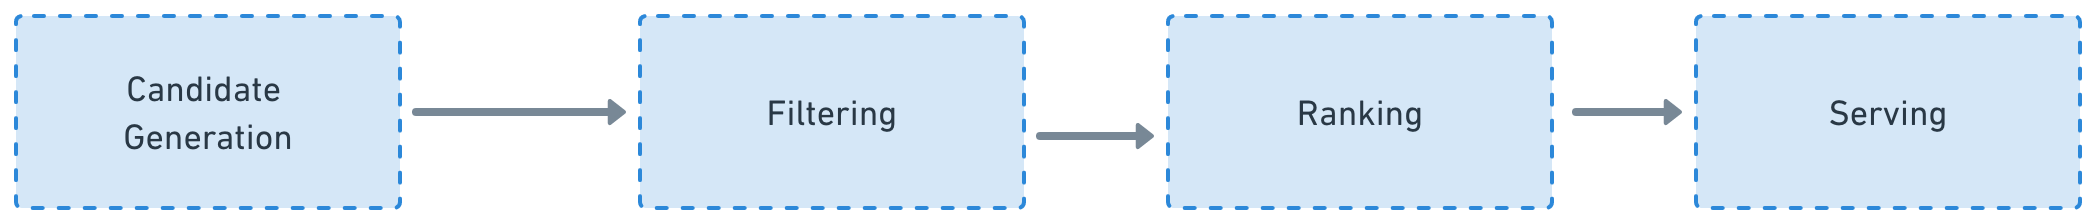
\includegraphics[width=\textwidth]{figures/recsys.png}
\caption{Recommender systems as a machine learning problem}
\end{figure}

\begin{formal}
\begin{itemize}
  \item \textbf{Candidate Generation} - First, we ingest data from the web app.  This data goes into the initial piece, which hosts our first-pass model generating \textbf{candidate recommendations}. This is where collaborative filtering takes place, and we whittle our list of potential candidates down from millions to thousands or hundreds.
  \item \textbf{Ranking} - Finally, we need a way to order the filtered list of recommendations based on what we think the user will prefer the most, so the next stage is \textbf{ranking}, and then we serve them out in the timeline or the ML product interface we're working with.
  \item \textbf{Filtering} - Once we have a generated list of candidates, we want to continue to filter them, using business logic (i.e. we don't want to see NSFW content, or items that are not on sale, for example.). This is generally a heavily heuristic-based step.
  \item \textbf{Retrieval} - This is the piece where the web application usually hits a model endpoint to get the final list of items served to the user through the product UI.
\end{itemize}
\end{formal}
    
Databases have become the fundamental tool in building backend infrastructure that performs data lookups. Embeddings have become similar building blocks in the creation of many modern search and recommendation product architectures. Embeddings are a type of \textbf{machine learning feature} --- or model input data --- that we use first as input into the feature engineering stage, and the first set of results that come from our candidate generation stage, that are then incorporated into downstream processing steps of ranking and retrieval to produce the final items the user sees.

\subsubsection{Machine learning features}

Now that we have a high-level conceptual view of how machine learning and recommender systems work, let's build towards a candidate generation model that will offer relevant flits.

Let's start by modeling a traditional machine learning problem and contrast it with our NLP problem. For example, let's say that one of our business problems is predicting whether a bird is likely to continue to stay on Flutter or to churn\footnote{An extremely common business problem to solve in almost every industry where either customer population or subscription based on revenues is important} --- disengage and leave the platform.

When we predict churn, we have a given set of machine learning feature inputs for each user and a final binary output of 1 or 0 from the model, 1 if the bird is likely to churn, or 0 if the user is likely to stay on the platform.

We might have the following inputs:

\begin{itemize}
  \item How many posts the bird has clicked through in the past month (we'll call this \mintinline{python}{bird_posts} in our input data)
  \item The geographical location of the bird from the browser headers (\mintinline{python}{bird_geo})
  \item How many posts the bird has liked over the past month (\mintinline{python}{bird_likes})
\end{itemize}



\begin{table}[H]
  \centering
    \caption{Tabular Input Data for Flutter Users}
\begin{tabular}{|l|l|l|l|}
\hline
\rowcolor[HTML]{D5E7F7}
bird\_id & bird\_posts & bird\_geo & bird\_likes \\ \hline
012 	 & 2  		 & US   	 & 5  		 \\ \hline
013 	 & 0  		 & UK   	 & 4  		 \\ \hline
056 	 & 57 		 & NZ   	 & 70 		 \\ \hline
612 	 & 0  		 & UK   	 & 120		 \\ \hline
\end{tabular}
\end{table}

We start by selecting our model features and arranging them in tabular format.  We can formulate this data as a table (which, if we look closely, is also a matrix) based on rows of the bird id and our bird features.

Tabular data is any structured data. For example, for a given Flutter user we have their user id, how many posts they've liked, how old the account is, and so on. This approach works well for what we consider traditional machine learning approaches which deal with tabular data.  As a general rule, the creation of the correct formulation of input data is perhaps the heart of machine learning. I.e. if we have bad input, we will get bad output. So in all cases, we want to spend our time putting together our input dataset and engineering features very carefully.

These are all discrete features that we can feed into our model and learn weights from, and is fairly easy as long as we have numerical features.  But, something important to note here is that, in our bird interaction data, we have both numerical and textual features (bird geography). So what do we do with these textual features? How do we compare "US" to "UK"?

The process of formatting data correctly to feed into a model is called \textbf{feature engineering}. When we have a single continuous, numerical feature, like “the age of the flit in days”, it’s easy to feed these features into a model. But, when we have textual data, we need to turn it into numerical representations so that we can compare these representations.  

\subsection{Numerical Feature Vectors}
Within the context of working with text in machine learning, we represent features as numerical vectors. We can think of each row in our tabular feature data as a vector. And a collection of features, or our tabular representation, is a matrix. For example, in the vector for our first user, \mintinline{python}{[012, 2, 'US', 5]}, we can see that this particular value is represented by four features. When we create vectors, we can run mathematical computations over them and use them as inputs into ML models in the numerical form we require.

Mathematically, vectors are collections of coordinates that tell us where a given point is in space among many dimensions. For example, in two dimensions, we have a point $[2,5]$, representing \mintinline{python}{bird_posts} and \mintinline{python}{bird_likes}.


In three dimensions, with three features including the bird id, we would have a vector
\begin{equation}
\begin{bmatrix}
12 & 2 & 5\\
\end{bmatrix}
\end{equation}
which tells us where that user falls on all three axes.

\begin{figure}[htbp]
\begin{adjustbox}{center}
\tdplotsetmaincoords{60}{120}
\begin{tikzpicture}
[scale=3, tdplot_main_coords, axis/.style={->,blue,thick},
vector/.style={-stealth,azure,very thick},
vector guide/.style={dashed,azure,thick}]

%standard tikz coordinate definition using x, y, z coords
\coordinate (O) at (0,0,0);

%tikz-3dplot coordinate definition using x, y, z coords

\pgfmathsetmacro{\ax}{.12}
\pgfmathsetmacro{\ay}{.2}
\pgfmathsetmacro{\az}{.5}

\coordinate (P) at (\ax,\ay,\az);

%draw axes
\draw[axis] (0,0,0) -- (1,0,0) node[anchor=north east]{$x$};
\draw[axis] (0,0,0) -- (0,1,0) node[anchor=north west]{$y$};
\draw[axis] (0,0,0) -- (0,0,1) node[anchor=south]{$z$};

%draw a vector from O to P
\draw[vector] (O) -- (P);

%draw guide lines to components
\draw[vector guide] (O) -- (\ax,\ay,0);
\draw[vector guide] (\ax,\ay,0) -- (P);
\draw[vector guide] (P) -- (0,0,\az);
\draw[vector guide] (\ax,\ay,0) -- (0,\ay,0);
\draw[vector guide] (\ax,\ay,0) -- (0,\ay,0);
\draw[vector guide] (\ax,\ay,0) -- (\ax,0,0);
\node[tdplot_main_coords,anchor=east]
at (\ax,0,0){(\ax, 0, 0)};
\node[tdplot_main_coords,anchor=west]
at (0,\ay,0){(0, \ay, 0)};
\node[tdplot_main_coords,anchor=south]
at (0,0,\az){(0, 0, \az)};
\end{tikzpicture}
\end{adjustbox}
\caption{Projecting a vector into the 3d space}
\label{fig:my_figure}
\end{figure}

But how do we represent "US" or "UK" in this space? Because modern models converge by performing operations on matrices  \citep{lakshmanan2020machine}, we need to encode geography as some sort of numerical value so that the model can calculate them as inputs\footnote{There are some models, specifically decision trees, where you don't need to do text encoding because the tree learns the categorical variables out of the box, however implementations differ, for example the two most popular implementations, scikit-learn and XGBoost \citep{altay_2020}, can't.}. So, once we have a combination of vectors, we can compare it to other points. So in our case, each row of data tells us where to position each bird in relation to any other given bird based on the combination of features.  And that's really what our numerical features allow us to do.


\subsection{From Words to Vectors in Three Easy Pieces}
In "Operating Systems: Three Easy Pieces", the authors write, "Like any system built by humans, good ideas accumulated in operating systems over time, as engineers learned what was important in their design." \citep{arpaci2018operating} Today's large language models were likewise built on hundreds of foundational ideas over the course of decades.  There are, similarly, several fundamental concepts that make up the work of transforming words to numerical representations.

These show up over and over again, in every deep learning architecture and every NLP-related task\footnote{When we talk about tasks in NLP-based machine learning, we mean very specifically, what the machine learning problem is formulated to do. For example, we have the task of ranking, recommendation, translation, text summarization, and so on.}:

\begin{formal}
\begin{itemize}
  \item \textbf{Encoding} - We need to represent our non-numerical, multimodal data as numbers so we can create models out of them. There are many different ways of doing this.
  \item \textbf{Vectors} - we need a way to store the data we have encoded and have the ability to perform mathematical functions in an optimized way on them. We store encodings as vectors, usually floating-point representations.
  \item \textbf{Lookup matrices} - Often times, the end-result we are looking for from encoding and embedding approaches is to give some approximation about the shape and format of our text, and we need to be able to quickly go from numerical to word representations across large chunks of text. So we use lookup tables, also known as hash tables, also known as attention, to help us map between the words and the numbers.
\end{itemize}
\end{formal}

As we go through the historical context of embeddings, we'll build our intuition from encoding to BERT and beyond\footnote{Original diagram from  \href{http://mccormickml.com/2019/11/11/bert-research-ep-1-key-concepts-and-sources/}{this excellent guide on BERT}}. What we'll find as we go further into the document is that the explanations for each concept get successively shorter, because we've already done the hard work of understanding the building blocks at the beginning.

\begin{figure}[H]
\centering
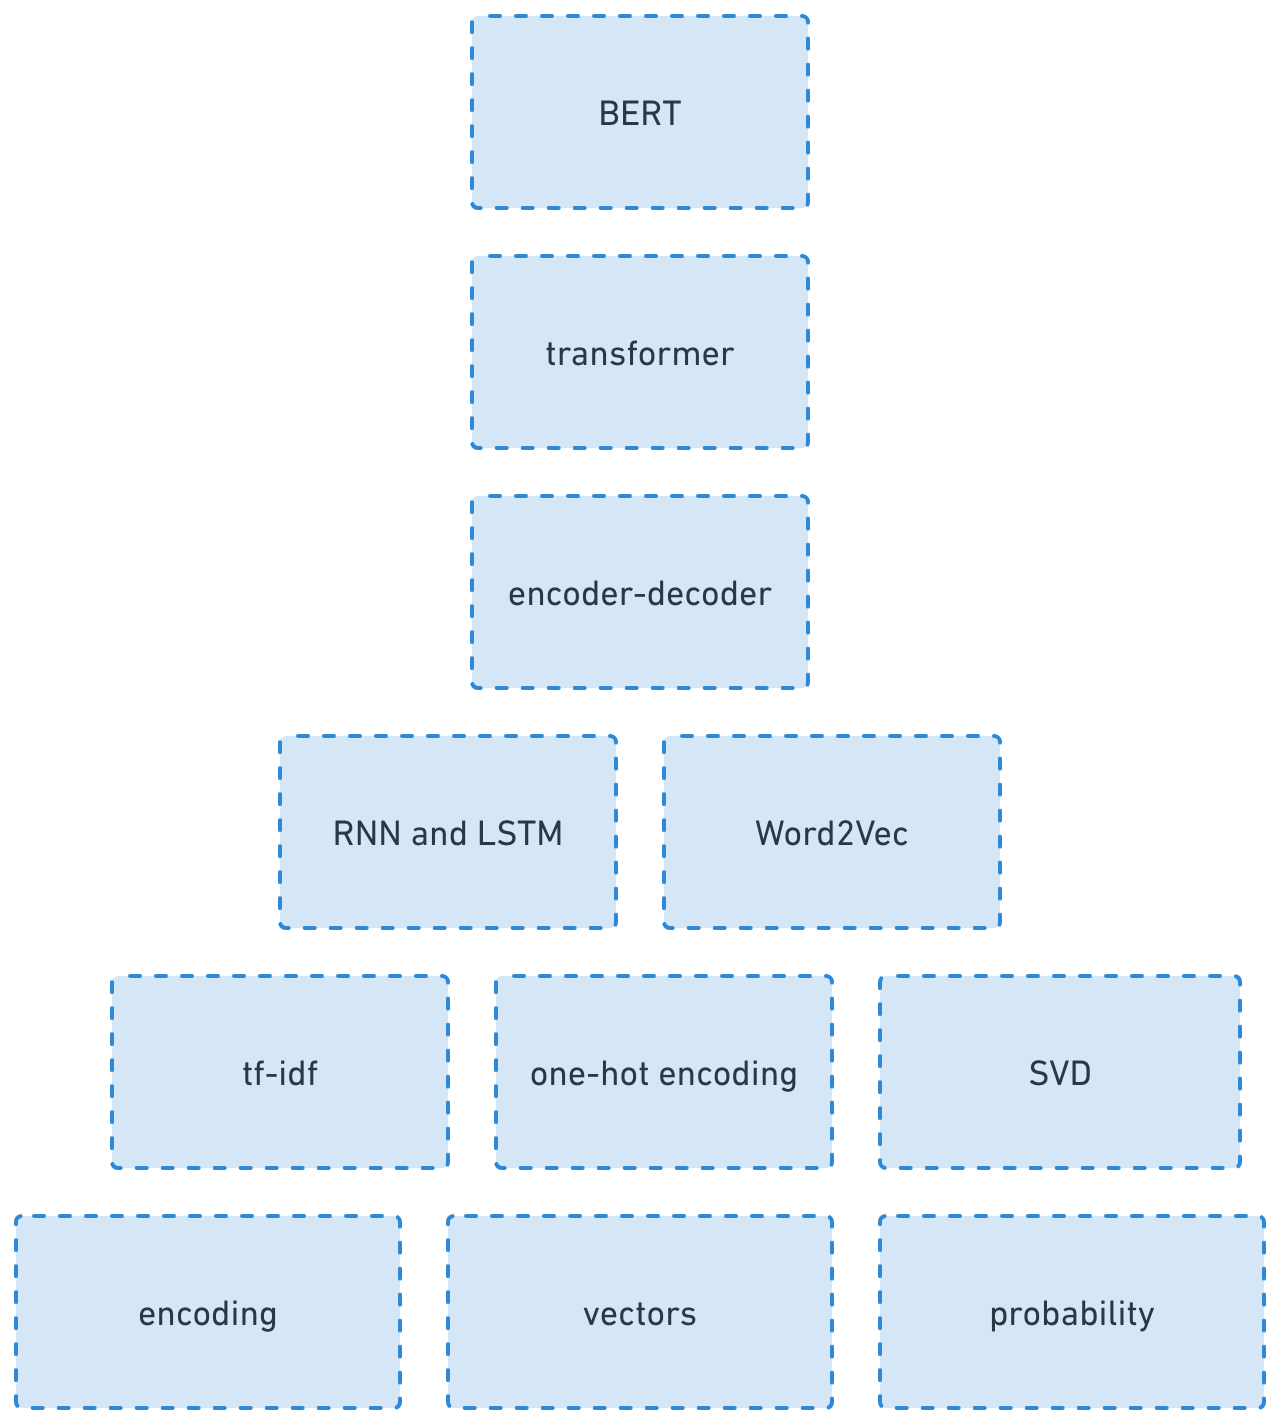
\includegraphics[width=.6\textwidth]{figures/pyramid.png}
\caption{Pyramid of fundamental concepts building to BERT}
\end{figure}

\section{Historical Encoding Approaches}

Compressing content into lower dimensions for compact numerical representations and calculations is not a new idea. For as long as humans have been overwhelmed by information, we've been trying to synthesize it so that we can make decisions based on it. Early approaches have included one-hot encoding, TF-IDF, bag-of-words, LSA, and LDA.

The earlier approaches were \textbf{count-based} methods. They focused on counting how many times a word appeared relative to other words and generating encodings based on that. LDA and LSA can be considered statistical approaches, but they are still concerned with inferring the properties of a dataset through heuristics rather than modeling. \textbf{Prediction-based} approaches came later and instead learned the properties of a given text through models  such as support vector machines, Word2Vec, BERT, and the GPT series of models, all of which use learned embeddings instead.

\begin{figure}[H]
    \centering
    \resizebox{1\textwidth}{!}{%
\begin{forest}
  for tree={
    align=center,
    parent anchor=south,
    child anchor=north,
    font=\sffamily,
    edge={->,thick},
    l sep+=20pt,
  }
  [\textbf{Embedding Methods}    [\textbf{Count-based Methods} 	 [\textbf{TF-IDF}]
      [\textbf{One-Hot Encoding}]
      [\textbf{Bag-of-words}]
      [\textbf{LSA}]
      [\textbf{LDA}]
    ]
    [\textbf{Prediction-based Methods} 	 [\textbf{SVM}]
      [\textbf{Word2Vec}]
      [\textbf{BERT family}]
      [\textbf{GPT family}]
    ]
  ]
\end{forest}}
	 \caption{Embedding Method Solution Space}
\end{figure}

\begin{formal}
\textbf{A Note on the Code}
In looking at these approaches programmatically, we'll start by using \mintinline{python}{scikit-learn}, the de-facto standard machine learning library for smaller datasets, with some implementations in native Python for clarity in understanding functionality that scikit-learn wraps.  As we move into deep learning, we'll move to PyTorch, a deep learning library that's quickly becoming industry-standard for deep learning implementation. There are many different ways of implementing the concepts we discuss here, these are just the easiest to illustrate using Python's ML lingua franca libraries.
\end{formal}

\subsection{Early Approaches}

The first approaches to generating textual features were count-based, relying on simple counts or high-level understanding of statistical properties: they were \textbf{descriptive} instead of models, which are \textbf{predictive} and attempt to guess a value based on a set of input values.  The first methods were \textbf{encoding methods}, a precursor to embedding. Encoding is often a process that still happens as the first stage of data preparation for input into more complex modeling approaches.  There are several methods to create text features using a process known as encoding so that we can map the geography feature into the vector space:

\begin{itemize}
  \item Ordinal encoding   
  \item Indicator encoding
  \item One-Hot encoding
\end{itemize}

In all these cases, what we are doing is creating a new feature that maps to the text feature column but is a numerical representation of the variable so that we can project it into that space for modeling purposes. We'll motivate these examples with simple code snippets from scikit-learn, the most common library for demonstrating basic ML concepts. We'll start with \textbf{count-based} approaches.

\subsection{Encoding}
\textbf{Ordinal encoding}
Let's again come back to our dataset of flits. We encode our data using sequential numbers. For example, "1" is "finch", "2" is "bluejay" and so on. We can use this method only if the variables have a natural ordered relationship to each other. For example, in this case "bluejay" is not "more" than "finch" and so would be incorrectly represented in our model. The case is the same, if, in our flit data, we encode "US" as 1 and "UK" as 2.

\begin{table}[H]
 \centering
    \caption{Bird Geographical Location Encoding}
\begin{tabular}{|>{\centering\arraybackslash}m{2cm}|>{\centering\arraybackslash}m{2cm}|>{\centering\arraybackslash}m{2cm}|>{\centering\arraybackslash}m{2cm}|>{\centering\arraybackslash}m{2.5cm}|}
\hline
\rowcolor[HTML]{D5E7F7}
bird\_id & bird\_posts & bird\_geo & bird\_likes & enc\_bird\_geo \\ \hline
012 	 & 2  		 & US   	 & 5  		 & 2         		 \\ \hline
013 	 & 0  		 & UK   	 & 4  		 & 1         		 \\ \hline
056 	 & 57 		 & NZ   	 & 70 		 & 0         		 \\ \hline
612 	 & 0  		 & UK   	 & 120		 & 1         		 \\ \hline
\end{tabular}
\end{table}

\begin{figure}[H]
\begin{minted}
[
frame=lines,
framesep=2mm,
baselinestretch=1.2,
fontsize=\footnotesize,
linenos
]{python3}
from sklearn.preprocessing import OrdinalEncoder

data = [['US'], ['UK'], ['NZ']]
>>> print(data)
[['US']
 ['UK']
 ['NZ']]
 
# our label features
encoder = OrdinalEncoder()
result = encoder.fit_transform(data)
>>> print(result)
[[2.]
 [1.]
 [0.]]
\end{minted}
\caption{Ordinal Encoding in Scikit-Learn \href{https://github.com/veekaybee/what_are_embeddings/blob/main/notebooks/fig_22_ordinal.ipynb}{source}}
\end{figure}

\subsubsection{Indicator and one-hot encoding}

Indicator encoding, given $n$ categories (i.e. "US", "UK", and "NZ"), encodes the variables into $n-1$ categories, creating a new feature for each category. So, if we have three variables, indicator encoding encodes into two indicator variables.  Why would we do this? If the categories are mutually exclusive, as they usually are in point-in-time geolocation estimates, if someone is in the US, we know for sure they're not in the UK and not in NZ, so it reduces computational overhead.

If we instead use all the variables and they are very closely correlated, there is a chance we'll fall into something known as the \textbf{indicator variable trap}. We can predict one variable from the others, which means we no longer have feature independence. This generally isn't a risk for geolocation since there are more than 2 or 3 and if you're not in the US, it's not guaranteed that you're in the UK. So, if we have US = 1, UK = 2, and NZ = 3, and prefer more compact representations, we can use indicator encoding.  However, many modern ML approaches don't require linear feature independence and use L1 regularization\footnote{Regularization is a way to prevent our model from \textbf{overfitting}. Overfitting means our model can exactly predict outcomes based on the training data, but it can't learn new inputs that we show it, which means it can't generalize} to prune feature inputs that don't minimize the error, and as such only use one-hot encoding.

\textbf{One-hot encoding} is the most commonly-used of the count-based methods. This process creates a new variable for each feature that we have.  Everywhere the element is present in the sentence, we place a “1” in the vector. We are creating a mapping of all the elements in the feature space, where $0$ indicates a non-match and $1$ indicates a match, and comparing how similar those vectors are.

\begin{figure}[H]
\begin{minted}
[
frame=lines,
framesep=2mm,
baselinestretch=1.2,
fontsize=\footnotesize,
linenos
]{python}
from sklearn.preprocessing import OneHotEncoder
import numpy as np

enc = OneHotEncoder(handle_unknown='ignore')
data = np.asarray([['US'], ['UK'], ['NZ']])
enc.fit(data)
enc.categories_
>>> [array(['NZ', 'UK', 'US'], dtype='<U2')]
onehotlabels = enc.transform(data).toarray()
onehotlabels
>>>
array([[0., 0., 1.],
  	 [0., 1., 0.],
  	 [1., 0., 0.]])
\end{minted}
\caption{One-Hot Encoding in scikit-learn\href{https://github.com/veekaybee/what_are_embeddings/blob/main/notebooks/fig_22_ordinal.ipynb}{source}}
\end{figure}


\begin{table}[H]
 \centering
    \caption{Our one-hot encoded data with labels}
\begin{tabular}{llll}
\hline
\rowcolor[HTML]{D5E7F7}  
bird\_id & US & UK & NZ \\
\hline
012 	 & 1  & 0  & 0  \\
\hline
013 	 & 0  & 1  & 0  \\
\hline
056 	 & 0  & 0  & 1
\end{tabular}
\end{table}


Now that we've encoded our textual features as vectors, we can feed them into the model we're developing to predict churn. The function we've been learning will minimize the loss of the model, or the distance between the model's prediction and the actual value, by predicting correct parameters for each of these features. The learned model will then return a value from 1 to 0 that is a probability that the event, either churn or no-churn, has taken place, given the input features of our particular bird.  Since this is a supervised model, we then evaluate this model for accuracy by feeding our test data into the model and comparing the model's prediction against the actual data, which tells us whether the bird has churned or not.

What we've built is a standard \textbf{logistic regression model}. Generally these days the machine learning community has converged on using gradient-boosted decision tree methods for dealing with tabular data, but we'll see that neural networks build on simple linear and logistic regression models to generate their output, so it's a good starting point.

\subsubsection*{Embeddings as larger feature inputs}

Once we have encoded our feature data, we can use this input for any type of model that accepts tabular features.  In our machine learning task, we were looking for output that indicated whether a bird was likely to leave the platform based on their location and some usage data. Now, we'd like to focus specifically on surfacing flits that are similar to other flits the user has already interacted with so we'll need feature representations of either/or our users or our content.

Let's go back to the original business question we posed at the beginning of this document: how do we recommend interesting new content for Flutter users given that we know that past content they consumed (i.e. liked and shared)?

In the traditional \textbf{collaborative filtering} approach to recommendations, we start by constructing a user-item matrix based on our input data that, when factored, gives us the latent properties of each flit and allows us to recommend similar ones.

In our case, we have Flutter users who might have liked a given flit. What other flits would we recommend given the textual properties of that one?

Here’s an example.  We have a flit that our bird users liked.

\begin{formal}
    "Hold fast to dreams, for if dreams die, life is a broken-winged bird that cannot fly."
\end{formal}

We also have other flits we may or may not want to surface in our bird's feed.

\begin{formal}
"No bird soars too high if he soars with his own wings."
\end{formal}

\begin{formal}
“A bird does not sing because it has an answer, it sings because it has a song.”
\end{formal}

How would we turn this into a machine learning problem that takes features as input and a prediction as an output, knowing what we know about how to do this already?  First, in order to build this matrix, we need to turn each word into a feature that's a column value and each user remains a row value.

\begin{flushleft}
The best way to think of the difference between tabular and free-form representations as model inputs is that a row of tabular data looks like this,\mintinline{python}{ [012,2,"US", 5]}, and a "row" or document of text data looks like this, \mintinline{python}{["No bird soars too high if he soars with his own wings."]} In both cases, each of these are vectors, or a list of values that represents a single bird.
\end{flushleft}

In traditional machine learning, rows are our user data about a single bird and columns are features about the bird. In recommendation systems, our rows are the individual data about each user, and our column data represents the given data about each flit.  If we can factor this matrix, that is decompose it into two matrices ($Q$ and $P^T$) that, when multiplied, the product is our original matrix ($R$), we can learn the "latent factors" or features that allow us to group similar users and items together to recommend them.

Another way to think about this is that in traditional ML, we have to actively engineer features, but they are then available to us as matrices. In text and deep-learning approaches, we don't need to do feature engineering, but need to perform the extra step of generating valuable numeric features anyway.


\begin{tikzpicture}[nmat/.style={matrix of mathsf nodes,inner sep=0pt,nodes in empty cells,column sep=-\pgflinewidth,
row sep=-\pgflinewidth,nodes={text height=1.7ex,text depth=0.2ex,inner
sep=2pt,minimum width=1.8ex},matrix dividers={thin},matrix
frame={thick}},font=\sffamily,
empty node/.style={fill=none}]
\matrix[nmat,nodes={fill=w_lightblue}] (mat1) {
1& & 3 &  &  & 5 &  &  & 5 &  & 4 &  \\
&  & 5 & 4  &  &  &  4&  &  & 2 & 1 & 3 \\
2  & 4 &  & 1 & 2  &  & 3 &  & 4 & 3 & 5 &  \\
& 2& 4 &  & 5 &  &  & 4 & &  &  2&  \\
&  & 4 & 3 & 4 & 2 &  &  &  &  & 2 &5  \\
1 &  & 3 &  & 3 &  &  &  2&  &  &  4& \\
};
\node[below=0.2ex of mat1,scale=2.5,blue] {$\mathsf{R}$};
\node[rotate=90,left=1.3ex of mat1,xshift=3em,blue] {users};
\node[above=0ex of mat1,xshift=1em,blue] {words};
\node[right=0.1ex of mat1,scale=2] (approx) {$\approx$};
\matrix[nmat,right=0.1ex of approx] (mat2) {
        	&  &  \\
        	&  &  \\
        	&  &  \\
        	&  &  \\
        	&  &  \\
        	&  & \\
};
\node[rotate=90,left=1.3ex of mat2,xshift=-1em,blue] {users};
\node[above=0ex of mat2,blue] {latent factors};
\node[below=0.2ex of mat2,scale=2.5,blue] {$\mathsf{Q}$};
\node[right=0.1ex of mat2,scale=2] (cdot) {$\times$};
\matrix[nmat,right=0.1ex of cdot] (mat3) {
        	&  &  &  &  &  &  &  &  &  &  &  \\
        	&  &  &  &  &  &  &  &  &  &  &  \\
        	&  &  &  &  &  &  &  &  &  &  & \\
};
\node[rotate=-90,right=1.5ex of mat3,xshift=-2em,blue] {latent factors};
\node[above=0ex of mat3,blue] {words};
\node[below=0.2ex of mat3,scale=2.5,blue] {$\mathsf{P^T}$};
\end{tikzpicture}


The factorization of our feature matrix into these two matrices, where the rows in Q are actually embeddings \citep{levy2014neural} for users and the rows in matrix P are embeddings for flits, allows us to fill in values for flits that Flutter users have not explicitly liked, and then perform a search across the matrix to find other words they might be interested in. The end-result is our generated recommendation candidates, which we then filter downstream and surface to the user because the core of the recommendation problem is to recommend items to the user.

In this base-case scenario, each column could be a single word in the entire vocabulary of every flit we have and the vector we create, shown in the matrix frequency table, would be an insanely large, sparse vector that has a $0$ of occurrence of words in our vocabulary. The way we can build toward this representation is to start with a structure known as a \textbf{bag of words}, or simply the frequency of appearance of text in a given document (in our case, each flit is a document.) This matrix is the input data structure for many of the early approaches to embedding.

In scikit-learn, we can create an initial matrix of our inputs across documents using `CountVectorizer`.


\begin{figure}[H]
\begin{minted}
[
frame=lines,
autogobble,
framesep=2mm,
baselinestretch=1.2,
fontsize=\footnotesize,
breaklines,
linenos
]{python}
from sklearn.feature_extraction.text import CountVectorizer
import pandas as pd

vect = CountVectorizer(binary=True)
vects = vect.fit_transform(flits)

responses = ["Hold fast to dreams, for if dreams die, life is a broken-winged bird that cannot fly.", "No bird soars too high if he soars with his own wings.", "A bird does not sing because it has an answer, it sings because it has a song."]

doc = pd.DataFrame(list(zip(responses)))

td = pd.DataFrame(vects.todense()).iloc[:5]  
td.columns = vect.get_feature_names_out()
term_document_matrix = td.T
term_document_matrix.columns = ['flit '+str(i) for i in range(1, 4)]
term_document_matrix['total_count'] = term_document_matrix.sum(axis=1)

print(term_document_matrix.drop(columns=['total_count']).head(10))

          flit_1  flit_2  flit_3
an         0       0       1
answer     0       0       1
because    0       0       1
bird       1       1       1
broken     1       0       0
cannot     1       0       0
die        1       0       0
does       0       0       1
dreams     1       0       0
fast       1       0       0


\end{minted}
\caption{Creating a matrix frequency table to create a user-item matrix
\href{https://github.com/veekaybee/what_are_embeddings/blob/main/notebooks/fig_22_ordinal.ipynb}{source}}
\end{figure}



\subsubsection{TF-IDF}

One-hot encoding just deals with presence and absence of a single term in a single document. However, when we have large amounts of data, we'd like to consider the weights of each term in relation to all the other terms in a collection of documents.

To address the limitations of one-hot encoding, TF-IDF, or term frequency-inverse document frequency was developed. TF-IDF was introduced in the 1970s\footnote{By Karen Spärck Jones, whose paper, \href{https://blog.babbar.tech/who-is-karen-sparck-jones/}{"Synonymy and semantic classification} is fundamental to the field of NLP} as a way to create a vector representation of a document by averaging all the document's word weights. It worked really well for a long time and still does in many cases.  For example, one of the most-used search functions, BM25, uses TF-IDF as a baseline  \citep{schutze2008introduction} as a default search strategy in Elasticsearch/Opensearch \footnote{You can read about how Elasticsearch implements BM25 \href{https://www.elastic.co/blog/practical-bm25-part-1-how-shards-affect-relevance-scoring-in-elasticsearch}{here}}. It extends TF-IDF to develop a probability associated with the probability of relevance for each pair of words in a document and it is still being applied in neural search today  \citep{svore2009machine}.  

TF-IDF will tell you how important a single word is in a corpus by assigning it a weight and, at the same time, down-weight common words like ,"a", "and", and "the". This calculated weight gives us a feature for a single word TF-IDF, and also the relevance of the features across the vocabulary.

We take all of our input data that's structured in sentences and break it up into individual words, and perform counts on its values, generating the bag of words. TF is term frequency, or the number of times a term appears in a document relative to the other terms in the document.

\begin{equation}
\mathrm{tf}(t,d) = \frac{f_{t,d}}{{\sum_{t' \in d}{f_{t',d}}}}
\end{equation}

And IDF is the inverse frequency of the term across all documents in our vocabulary.

\begin{equation}
\mathrm{idf}(t, D) =  \log \frac{N}{|\{d \in D: t \in d\}|}
\end{equation}

Let's take a look at how to implement it from scratch:

\begin{figure}[H]
\begin{minted}
[
frame=lines,
framesep=2mm,
baselinestretch=1.2,
fontsize=\footnotesize,
breaklines,
linenos
]{python}

import math

# Process documents into individual words
documentA  = ['Hold','fast','to','dreams','for','if','dreams','die,' ,'life','is','a','broken-winged','bird','that','cannot','fly']
documentB =  ['No','bird','soars','too','high','if', 'he','soars','with','his','own','wings']

def tf(doc_dict: dict, doc_elements: list[str]) -> dict:
	"""Term frequency of a word in a document  over total words in document"""
	tf_dict = {}
	corpus_count = len(doc_elements)
	for word, count in doc_dict.items():
    	tf_dict[word] = count / float(corpus_count)  
	return tf_dict

def idf(doc_list: list[str]) -> dict:
	"""The number of documents in which the term appears per term"""
	idf_dict = {}
	N = len(doc_list)
	idf_dict = dict.fromkeys(doc_list[0].keys(), 0)
	for word, val in idf_dict.items():
    	idf_dict[word] = math.log10(N / (float(val) + 1))
	return idf_dict

# All inverse document frequencies for all words
idfs = idf([dict_a, dict_b])

def tfidf(doc_elements: list[str], idfs)-> dict:
	"""TF * IDF per word given a single word and number of docs the term appears"""
	tfidf_dict = {}
	for word, val in doc_elements.items():
    	tfidf_dict[word] = val * idfs[word]
	return tfidf_dict

# Calculate the term frequency for each document individually
tf_a = tf(dict_a, document_a)
tf_b = tf(dict_b, document_b)

# Calculate the inverse document frequency given each term frequency
tfidf_a = tfidf(tf_a, idfs)
tfidf_b = tfidf(tf_b, idfs)

# Return weight of each word in each document wrt to the total corpus
document_tfidf = pd.DataFrame([tfidf_a, tfidf_b])
document_tfidf.T
# 	    doc 0      doc 1
    a        0.018814   0.000000
    dreams   0.037629   0.000000
    No       0.000000   0.025086
    Hold     0.018814   0.000000
\end{minted}
\caption{Truncated implementation of TF-IDF, see full \href{https://github.com/veekaybee/what_are_embeddings/blob/main/notebooks/fig_24_tf_idf_from_scratch.ipynb} {source}}
\end{figure}

Once we understand the underlying fundamental concept, we can use the scikit-learn implementation which does the same thing, and also surfaces the TF-IDF of each word in the vocabulary.

\begin{figure}[H]
\begin{minted}
[
frame=lines,
framesep=2mm,
baselinestretch=1.2,
fontsize=\footnotesize,
breaklines,
linenos
]{python}
from sklearn.feature_extraction.text import TfidfVectorizer
corpus = [
	"Hold fast to dreams, for if dreams die, life is a broken-winged bird that cannot fly.",
	"No bird soars too high if he soars with his own wings.",
]

text_titles = ["quote_langstonhughes", "quote_william_blake"]

vectorizer = TfidfVectorizer()
vector = vectorizer.fit_transform(corpus)
dict(zip(vectorizer.get_feature_names_out(), X.toarray()[0]))

tfidf_df = pd.DataFrame(vector.toarray(), index=text_titles, columns=vectorizer.get_feature_names_out())

tfidf_df.loc['00_Document Frequency'] = (tfidf_df > 0).sum()
tfidf_df.T

# How common or unique a word is in a given document wrt to the vocabulary
dreams_langstonhughes    quote_william_blake    00_Document Frequency
bird                    0.172503              0.197242              2.0
broken                  0.242447              0.000000              1.0
cannot                  0.242447              0.000000              1.0
die                     0.242447              0.000000              1.0
\end{minted}
\caption{Implementation of TF-IDF in scikit-learn \href{https://github.com/veekaybee/what_are_embeddings/blob/main/notebooks/fig_24_tf_idf_from_scratch.ipynb}{source}}
\end{figure}

Given that inverse document frequency is a measure of whether the word is common or not across the documents, we can see that "dreams" is important because they are rare across the documents and therefore interesting to us more so than "bird."We see that the tf-idf for a given word, "dreams", is slightly different for each of these implementations, and that's because Scikit-learn normalizes the denominator and uses \href{https://scikit-learn.org/stable/modules/generated/sklearn.feature_extraction.text.TfidfTransformer.html#sklearn.feature_extraction.text.TfidfTransformer}{a slightly different formula.}  You'll also note that in the first implementation we separate the corpus words ourselves, don't remove any stop words, and don't lowercase everything. Many of these steps are done automatically in scikit-learn or can be set as parameters into the processing pipeline. We'll see later that these are critical NLP steps that we perform each time we work with text.

TF-IDF enforces several important ordering rules on our text corpus:

\begin{itemize}
  \item Uprank term frequency when it occurs many times in a small number of documents
  \item Downrank term frequency when it occurs many times in many documents, aka is not relevant
  \item Really downrank the term when it appears across your entire document base \citep{schutze2008introduction}.
\end{itemize}

There are numerous ways to calculate and create weights for individual words in TF-IDF. In each case, we calculate a score for each word that tells us how important that word is in relation to each other word in our corpus, which gives it a weight. Once we figure out how common each word is in the set of all possible flits and get a weighted score for the entire sentence in relation to other sentences.

Generally, when we work with textual representations, we’re trying to understand which words, phrases, or concepts are similar to each other. Within our specific recommendations task, we are trying to understand which pieces of content are similar to each other, so that we can recommend content that users will like based on either their item history or the user history of users similar to them.

So, when we perform embedding in the context of recommender systems, we are looking to create neighborhoods from items and users, based on the activity of those users on our platform.  This is the initial solution to the problem of “how do we recommend flits that are similar to flit that the user has liked.” This is the process of collaborative filtering.

There are many approaches to collaborative filtering including a neighborhood-based approach,  which looks at weighted averages of user ratings and computes \textbf{cosine similarity}, between users.  It then finds groups, or neighborhoods of users which are similar to each other.

A key problem that makes up the fundamental problem in collaborative filtering and in recommendation systems in general is the ability to find similar sets of items among very large collections \citep{leskovec2020mining}.

Mathematically, we can do this by looking at the distance metric between any two given sets of items, and there are a number of different approaches, including  Euclidean distance, edit distance (more specifically, Levenshtein distance and Hamming distance), cosine distance, and more advanced compression approaches like \textbf{minhashing}.

The most commonly used approach in most models where we're trying to ascertain the semantic closeness of two items is \textbf{cosine similarity}, which is the cosine of the angle between two objects represented as vectors, bounded between -1 and 1. -1 means the two items are completely "opposite" of each other and 1 means they are completely the same item, assuming unit length. Zero means that you should probably use a distance measure other than cosine similarity because the vectors are completely orthogonal to each other. One point of clarification here is that cosine distance is the actual distance measure and is calculated as $1 - {similarity}(\vec{a}, \vec{b})$.

\begin{equation}
\mathrm{similarity}(\vec{a}, \vec{b}) = \frac{\vec{a} \cdot \vec{b}}{|\vec{a}| |\vec{b}|} = \frac{\sum\limits_{i=1}^{n} a_i b_i}{\sqrt{\sum\limits_{i=1}^{n} a_i^2} \sqrt{\sum\limits_{i=1}^{n} b_i^2}}
\end{equation}

We use cosine similarity over other measures like Euclidean distance for large text corpuses, for example, because in very large, sparse spaces, the direction of the vectors is just as, and even more important, than the actual values.

The higher the cosine similarity is for two words or documents, the better. We can use TF-IDF as a  way to look at cosine similarity. Once we've given each of our words a tf-idf score, we can also assign a vector to each word in our sentence, and create a vector out of each quote to assess how similar they are.


\begin{figure}[h]
    \centering
    \begin{tikzpicture}[scale=2]
   	 \draw[->] (0,0) -- (1.2,0) node[right]{$x$};
   	 \draw[->] (0,0) -- (0,1.2) node[above]{$y$};
   	 \draw[->,thick,blue] (0,0) -- (1,0.6) node[right]{$\text{bird}$};
   	 \draw[->,thick,azure] (0,0) -- (0.6,1) node[above]{$\text{wings}$};
   	 \draw[dashed] (0.6,0) -- (0.6,1);
   	 \draw[dashed] (0,0.6) -- (0.6,0.6);
   	 \draw[<->,thick] (0.3,0) arc (0:53:0.3) node[midway,right]{$\theta$};
   	 \node at (0.3,0.3) {$\theta$};
   	 \node at (0.2,0.2) {$\phi$};
    \end{tikzpicture}
    \caption{Illustration of cosine similarity between $\text{bird}$ and $\text{wings}$ vectors.}
    \label{fig:cosine-similarity}
\end{figure}

Let's take a look at the actual equation for cosine similarity. We start with the dot product between two vectors, which is just the sum of each value multiplied by the corresponding value in our second vector, and then we divide by the normalized dot product.

\begin{figure}[H]
\begin{minted}
[
frame=lines,
framesep=2mm,
baselinestretch=1.2,
fontsize=\footnotesize,
linenos
]{python}
v1 = [0,3,4,5,6]
v2 = [4,5,6,7,8]

def dot(v1, v2):
	dot_product = sum((a * b) for a,b in zip(v1,v2))
	return dot_product

def cosine_similarity(v1, v2):
	'''
	(v1 dot v2)/||v1|| *||v2||)
	'''
	products = dot(v1,v2)
	denominator = ( (dot(v1,v1) **.5) * (dot(v2,v2) ** .5) )
	similarity = products / denominator
	return similarity

print(cosine_similarity(v1, v2))
# 0.9544074144996451
\end{minted}
\caption{Implementation of cosine similarity from scratch
\href{https://github.com/veekaybee/what_are_embeddings/blob/main/notebooks/fig_29_cos_sim_from_scratch.ipynb}{source}}
\end{figure}

Or, once again, in scikit-learn, as a pairwise metric:

\begin{figure}[H]
\begin{minted}
[
frame=lines,
framesep=2mm,
baselinestretch=1.2,
fontsize=\footnotesize,
linenos
]{python}
from sklearn.metrics import pairwise

v1 = [0,3,4,5,6]
v2 = [4,5,6,7,8]

# need to be in numpy data format
pairwise.cosine_similarity([v1],[v2])
# array([[0.95440741]])

\end{minted}
\caption{Implementation of cosine similarity in scikit\href{https://github.com/veekaybee/what_are_embeddings/blob/main/notebooks/fig_29_cos_sim_from_scratch.ipynb}{source}}
\end{figure}

Other commonly-used distance measures in semantic similarity and recommendations include:

\begin{formal}
\begin{itemize}
  \item Euclidean distance - calculates the straight-line distance between two points
  \item Manhattan Distance - Measures the distance between two points by summing the absolute differences of their coordinates
  \item Jaccard Distance - Computes the dissimilarity between two sets by dividing the size of their intersection by the size of their union.
  \item Hamming Distance  - Measures the dissimilarity between two strings by counting the positions in which they differ
\end{itemize}
\end{formal}

\subsubsection{SVD and PCA}

There is a problem with the vectors we created in one-hot encoding and TF-IDF: they are sparse. A sparse vector is one that is mostly populated by zeroes. They are sparse because most sentences don't contain all the same words as other sentences. For example, in our flit, we might encounter the word "bird" in two sentences simultaneously, but the rest of the words will be completely different.

\begin{figure}[H]
\begin{minted}
[
frame=lines,
framesep=2mm,
baselinestretch=1.2,
fontsize=\footnotesize,
linenos
]{python}
sparse_vector = [1,0,0,0,0,0,0,0,0,0]
dense_vector = [1,2,2,3,0,4,5,8,8,5]
\end{minted}
\caption{Two types of vectors in text processing}
\end{figure}


Sparse vectors result in a number of problems, among these \textbf{cold start}---the idea that we don't know to recommend items that haven't been interacted with, or for users who are new. What we'd like, instead, is to create dense vectors, which will  give us more information about the data, the most important of which is accounting for the weight of a given word in proportion to other words. This is where we leave one-hot encodings and TD-IDF to move into approaches that are meant to solve for this sparsity. Dense vectors are just vectors that have mostly non-zero values. We call these dense representations dynamic representations \citep{Wang2020FromST}.


Several other related early approaches were used in lieu of TF-IDF for creating compact representations of items: \textbf{principal components analysis} (PCA) and \textbf{singular value decomposition} (SVD).  

SVD and PCA are both dimensionality reduction techniques that, applied through matrix transformations to our original text input data, show us the latent relationship between two items by breaking items down into latent components through matrix transformations.   

SVD is a type of matrix factorization that represents a given input feature matrix as the product of three matrices.  It then uses the component matrices to create linear combinations of features that are the largest differences from each other and which are directionally different based on the variance of the clusters of points from a given line.   Those clusters represent the “feature clusters” of the compressed features.  

In the process of performing SVD and decomposing these matrices, we generate a matrix representation that includes the eigenvectors and eigenvalue pairs or the sample covariance pairs.

PCA uses the same initial input feature matrix, but whereas one-hot encoding simply converts the text features into numerical features that we can work with, PCA also performs compression and projects our items into a two-dimensional feature space.  The first principal component is the scaled eigenvector of the data, the weights of the variables that describe your data best, and the second is the weights of the next set of variables that describe your data best.

The resulting model is a projection of all the words, clustered into a single space based on these dimensions. While we can't get individual meanings of all these components, it’s clear that the clusters of words, aka features, are \textbf{semantically similar}, that is they are close to each other in meaning\footnote{There are many definitions of semantic similarity - what does it mean for "king" and "queen" to be close to each other? - but a high-level approach involves using original sources like thesauri and dictionaries to create a structured knowledge base and offer a structured representation of terms and concepts based on nodes and edges, aka how often they appear near each other. \cite{chandrasekaran2021evolution}}.
 
The difference between the two is often confusing (people admitted as much in the 80s \cite{gerbrands1981relationships} when these approaches were still being worked out), and for the purposes of this survey paper we'll say that PCA can often be implemented using SVD \footnote{\href{https://scikit-learn.org/stable/modules/generated/sklearn.decomposition.PCA.html}{This is how it's implemented in the scikit-learn package}}.  


\subsection{LDA and LSA}

Because PCA performs computation on each combination of features to generate the two dimensions, it becomes immensely computationally expensive as the number of features grows.  Many of these early methods, like PCA, worked well for smaller datasets, like many of the ones used in traditional NLP research,  but as datasets continued to grow, they didn’t quite scale.  

Other approaches grew out of TF-IDF and PCA to address their limitations, including \textbf{latent semantic analysis} (LSA) and \textbf{latent Dirichlet allocation} (LDA) \cite{cvitanic2016lda}.  Both of these approaches start with the input document matrix that we built in the last section. The underlying principle behind both of these models is that words that occur close together more frequently have more important relationships. LSA uses the same word weighting that we used for TF-IDF and looks to combine that matrix into a lower rank matrix, a cosine similarity matrix. In the matrix, the values for the cells range from [-1,1], where -1 represents documents that are complete opposites and 1 means the documents are identical. LSA then runs over the matrix and groups items together.  

LDA takes a slightly different approach. Although it uses the same matrix for input, it instead outputs a matrix where the rows are words and columns are documents. The distance measure, instead of cosine similarity, is the numerical value for the topic that the intersection of the word and document provide.  The assumption is that any sentence we input will contain a collection of topics, based on proportions of representation in relation to the input corpus, and that there are a number of topics that we can use to classify a given sentence. We initialize the algorithm by assuming that there is a non-zero probability that each word could appear in a topic. LDA initially assigns words to topics at random, and then iterates until it converges to a point where it maximizes the probability for assigning a current word to a current topic.  In order to do the word-to-topic mapping, LDA generates an embedding that creates a space of clusters of words or sentences that work together semantically.

\subsection{Limitations of traditional approaches}
 
 All of these traditional methods look to address the problem of generating relationships between items in our corpus in various ways in the latent space - the relationships between words that are not explicitly stated but that we can tease out based on how we model the data.
 
 However, in all these cases, as our corpus starts to grow, we start to run into two problems: the curse of dimensionality and compute scale.
 
 \subsubsection{The curse of dimensionality}

As we one-hot encode more features, our tabular data set grows. Going back to our churn model,  what happens once we have 181 instead of two or three countries? We'll have to encode each of them  into their own vector representations. What happens if we have millions of vocabulary words, for example thousands of birds posting millions of messages every day? Our sparse matrix for tf-idf becomes computationally intensive to factor.

Whereas our input vectors for tabular machine learning and naive text approaches is only three entries because we only use three features, multimodal data effectively has a dimensionality of the number of written words in existence and image data has a dimensionality of height times width in pixels, for each given image. Video and audio data have similar exponential properties.  We can profile the performance of any code we write using \textbf{Big O notation}, which will classify an algorithm's runtime.  There are programs that perform worse and those that perform better based on the number of elements the program processes. This means that one-hot encodings, in terms of computing performance, are \begin{math}O(n)\end{math} in the worst case complexity. So, if our text is a corpus of a million unique words, we'll get to a million columns, or vectors, each of which will be sparse, since most sentences will not contain the words of other sentences.   

Let's take a more concrete case. Even in our simple case of our initial bird quote, we have 28 features, one for each word in the sentence, assuming we don't remove and process the most common \textbf{stop words} --- extremely common words like "the", "who", and "is" that appear in most texts but don't add semantic meaning.  How can we create a model that has 28 features? That's fairly simple if tedious - we encode each word as a numerical value.

  \begin{table}[H]
    \centering
   	 \caption{One-hot encoding and the growing curse of dimensionality for our flit}
\begin{tabular}{|l|l|l|l|l|l|l|l|}
\hline
\rowcolor[HTML]{D5E7F7}  
flit\_id & bird\_id & hold & fast & dreams & die & life & bird \\ \hline
9823420  & 012  & 1   & 1    & 1 	 & 1  & 1   	 & 1   \\ \hline
9823421  & 013  & 1   & 0    & 0 	 & 0  & 0   	 & 1   \\ \hline
\end{tabular}

\end{table}

Not only will it be hard to run computations over a linearly increasing set, once we start generating a large number of features (columns), we start running into the \textbf{curse of dimensionality}, which means that, the more features we accumulate, the more data we need in order to accurately statistically confidently say anything about them, which results in models that may not accurately represent our data \citep{houle2010can} if we have extremely sparse features, which is generally the case in user/item interactions in recommendations.   

\subsubsection{Computational complexity}
 
In production machine learning systems, the statistical properties of our algorithm are important. But just as critical is how quickly our model returns data, or the system's efficiency. System efficiency can be measured in many ways, and it is critical in any well-performing system to find the performance bottleneck that leads to latency, or the time spent waiting before an operation is  performed \citep{gregg2014systems}. If you have a recommendation system in production, you cannot risk showing the user an empty feed or a feed that takes more than a few milliseconds to render. If you have a search system, you cannot risk the results taking more than a few milliseconds to return, particularly in e-commerce settings \cite{arapakis2014impact}.  From the holistic systems perspective then, we can also have latency in how long it takes to generate data for a model, read in data, and train the model.

The two big drivers of latency are:

\begin{itemize}
  \item I/O processing - We can only send as many items over the network as our network speed allows
  \item CPU processing - We can only process as many items as we have memory available to us in any given system\footnote{there has been \href{https://benhoyt.com/writings/io-is-no-longer-the-bottleneck/}{discussion} over the past few years on whether IO or CPU are really the bottleneck in any modern data-intensive application.}
\end{itemize}


Generally, TF-IDF performs well in terms of identifying key terms in the document. However, since the algorithm processes all the elements in a given corpus, the time complexity grows for both the numerator and the denominator in the equation and overall, the time-complexity of computing the TF-IDF weights for all the terms in all the documents is $O(Nd)$, where $N$ is the total number of terms in the corpus and $d$ is the number of documents in the corpus. Additionally, because TF-IDF creates a matrix as output, what we end up doing is processing enormous state matrices. For example, if you have ~100k documents and need to store frequency counts and features for the top five thousand words appearing in those documents, we get a matrix of size $100000*5000$. This complexity only grows.

This linear time complexity growth becomes an issue when we're trying to process millions or hundreds of millions of \textbf{tokens} -- usually a synonym for words but can also be sub-words such as syllables. This is a problem that became especially prevalent as, over time in industry, storage became cheap.

From newsgroups to emails, and finally, to public internet text, we began to generate a lot of digital exhaust and companies collected it in the form of append-only logs \citep{kreps2014heart}, a sequence of records ordered by time, that's configured to continuously append records.\footnote{Jay Kreps' \href{https://engineering.linkedin.com/distributed-systems/log-what-every-software-engineer-should-know-about-real-time-datas-unifying}{canonical posts} on how logging works are a must-read} .

Companies started emitting, keeping, and using these endless log streams for data analysis and machine learning. All of a sudden, the algorithms that had worked well on a collection of less than a million documents struggled to keep up.

Capturing log data at scale began the rise of the Big Data era, which resulted in a great deal of variety, velocity, and volume of data movement. The rise in data volumes coincided with data storage becoming much cheaper, enabling companies to store everything they collected on racks of commodity hardware.

Companies were already retaining analytical data needed to run critical business operations in relational databases, but access to that data was structured and processed in batch increments on a daily or weekly basis. This new logfile data moved quickly, and with a level of variety absent from traditional databases.

The resulting corpuses for NLP, search, and recommendation problems also exploded in size, leading people to look for more performant solutions.  


\subsection{Support Vector Machines}

The first modeling approaches were \textbf{shallow} models --- models that perform machine learning tasks using only one layer of weights and biases \citep{collobert2008unified}. \textbf{Support vector machines} (SVM), developed at Bell Laboratories in the mid-1990s,  were used in high-dimensional spaces for NLP tasks like text categorization \citep{joachims2005text}. SVMs separate data clusters into points that are linearly separable by a \textbf{hyperplane}, a decision boundary that separates elements into separate classes. In a two-dimensional vector space, the hyperplane is a line, in a three or more dimensional space, the separator also comes in many dimensions.

The goal of the SVM is to find the optimal hyperplane such that the distance between new projections of objects (words in our case) into the space maximizes the distance between the plane and the elements so there's less chance of mis-classifying them.

\begin{figure}[H]
\centering
\tikzset{
    leftNode/.style={circle,minimum width=.5ex, fill=w_lightblue,draw},
    rightNode/.style={circle,minimum width=.5ex, fill=black,thick,draw},
    rightNodeInLine/.style={solid,circle,minimum width=.7ex, fill=black,thick,draw=white},
    leftNodeInLine/.style={solid,circle,minimum width=.7ex, fill=w_lightblue,thick,draw},
  }
\begin{tikzpicture}[
   	 scale=2,
   	 important line/.style={thick}, dashed line/.style={dashed, thin},
   	 every node/.style={color=black},
    ]
    \draw[dashed line, yshift=.7cm]
  	 (.2,.2) coordinate (sls) -- (2.5,2.5) coordinate (sle)
  	 node[solid,circle,minimum width=2.8ex,fill=none,thick,draw] (name) at (2,2){}
  	 node[leftNodeInLine] (name) at (2,2){}
  	 node[solid,circle,minimum width=2.8ex,fill=none,thick,draw] (name) at (1.5,1.5){}
  	 node[leftNodeInLine] (name) at (1.5,1.5){}
  	 node [above right] {$w\cdot x + b > 1$};

    \draw[important line]
  	 (.7,.7) coordinate (lines) -- (3,3) coordinate (linee)
  	 node [above right] {$w\cdot x + b = 0$};

    \draw[dashed line, xshift=.7cm]
  	 (.2,.2) coordinate (ils) -- (2.5,2.5) coordinate (ile)
  	 node[solid,circle,minimum width=2.8ex,fill=w_lightblue,thick,draw] (name) at (1.8,1.8){}
  	 node[rightNodeInLine] (name) at (1.8,1.8){}
  	 node [above right] {$w\cdot x + b < -1$};

    \draw[very thick,<->] ($(sls)+(.2,.2)$) -- ($(ils)+(.2,.2)$)
  	 node[sloped,above, near end] {Margin};

    \foreach \Point in {(.9,2.4), (1.3,2.5), (1.3,2.1), (2,3), (1,2.9)}{
      \draw \Point node[leftNode]{};
    }

    \foreach \Point in {(2.9,1.4), (2.3,.5), (3.3,.1), (2,0.9), (2.5,1)}{
      \draw \Point node[rightNode]{};
    }
\end{tikzpicture}
\caption{Example of points in the vector space in an SVM separated by a hyperplane}
\end{figure}


Examples of supervised machine learning tasks performed with SVMs included next word prediction, predicting the missing word in a given sequence, and predicting words that occur in a window. As an example, the classical word embedding inference task is autocorrect when we're typing on our phones. We type a word, and it's the job of the autocorrect to predict the correct word based on both the word itself and the surrounding context in the sentence. It therefore needs to learn a vocabulary of embeddings that will give it probabilities that it is selecting the correct word.

However, as in other cases, when we reach high dimensions, SVMs completely fail to work with sparse data because they rely on computing distances between points to determine the decision boundaries. Because in our sparse vector representations of elements most of the distances are zero, the hyperplane will fail to cleanly separate the boundaries and classify words incorrectly.

\subsection{Word2Vec}

To get around the limitations of earlier textual approaches and keep up with growing size of text corpuses, in 2013, researchers at Google came up with an elegant solution to this problem using neural networks, called Word2Vec \citep{mikolov2013efficient}.  

So far, we've moved from simple heuristics like one-hot encoding, to machine learning approaches like LSA and LDA that look to learn a dataset's modeled features.  Previously, like our original one-hot encodings, all the approaches to embedding focused on generating sparse vectors that can give an indication that two words are related, but not that there is a semantic relationship between them. For example, “The dog chased the cat” and “the cat chased the dog” would have the same distance in the vector space, even though they’re two completely different sentences.

Word2Vec is a family of models that has several implementations, each of which focus on transforming the entire input dataset into vector representations and, more importantly, focusing  not only on the inherent labels of individual words, but on the relationship between those representations.

There are two modeling approaches to Word2Vec - \textbf{continuous bag of words} (CBOW) and \textbf{skipgrams}, both of which generate dense vectors of embeddings but model the problem slightly differently. The end-goal of the Word2Vec model in either case is to learn the parameters that maximize that probability of a given word or group of words being an accurate prediction  \citep{goldberg2014word2vec}.

In training skipgrams, we take a word from the initial input corpus and predict the probability that a given set of words surround it. In the case of our initial flit quote, "Hold fast to dreams for if dreams die, life is a broken-winged bird that cannot fly", the model's intermediate steps generate a set of embeddings that's the distance between all the words in the dataset and fill in the next several probabilities for the entire phrase, using the word "fast" as input.  

\begin{figure}[H]
   	 \center{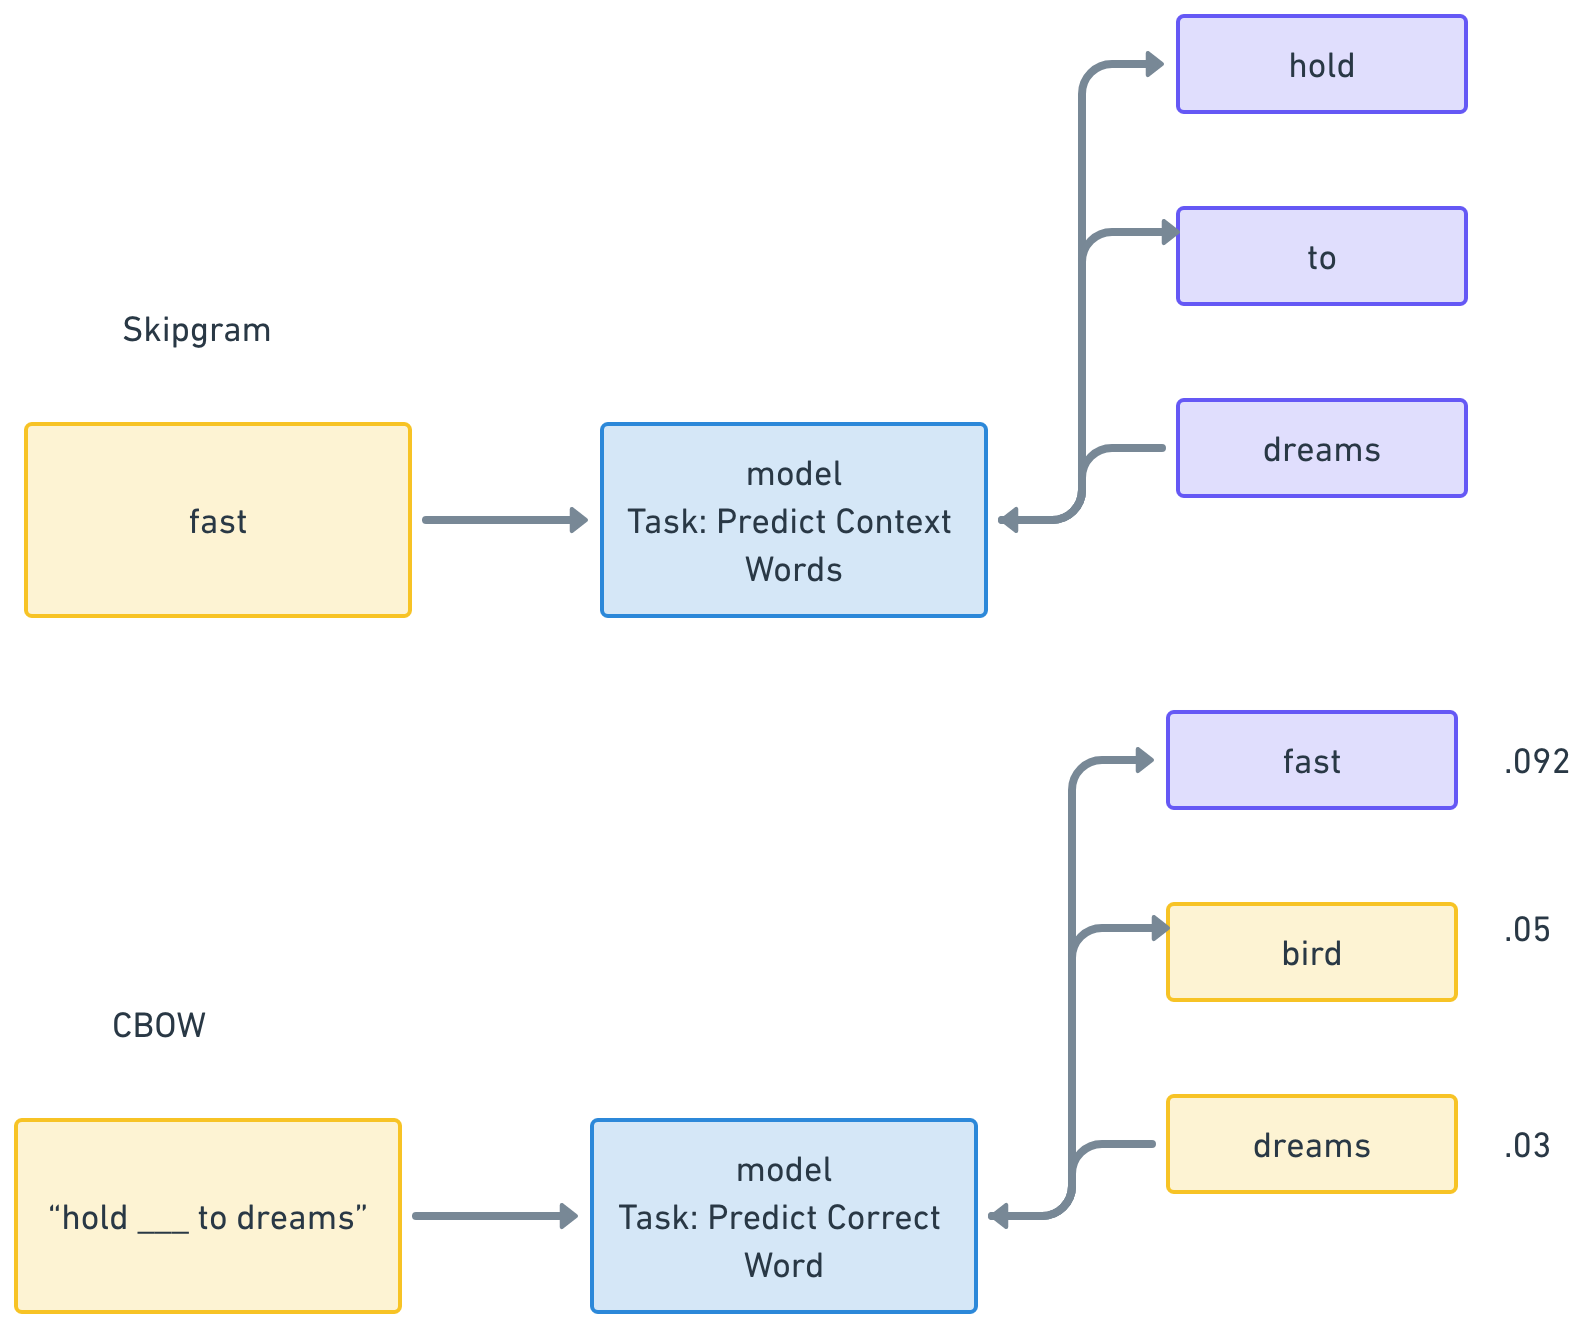
\includegraphics[width=\textwidth]
   	 {figures/word2vec.png}}
   	 \caption{Word2Vec Architecture}
      \end{figure}

In training CBOW, we do the opposite: we remove a word from the middle of a phrase known as the \textbf{context window} and train  a model to predict the probability that a given word fills the blank, shown in the equation below where we attempt to maximize.

\begin{equation}
\arg\max_\theta \prod_{w\in Text}\left[\prod_{c \in C(w)} p(c|w;\theta)\right]
\end{equation}

If we optimize these parameters - theta and Pi - and maximize the probability that the word belongs in the sentences, we'll learn good embeddings for our input corpus.

Let's focus on a detailed implementation of CBOW to better understand how this works. This time, for the code portion, we'll move on from scikit-learn, which works great for smaller data, to PyTorch for neural net operations.  

At a high level, we have a list of input words that are processed through a second layer, the embedding layer, and then through the output layer, which is just a linear model that returns probabilities.

\def\layersep{2.5cm}
 \begin{figure}[H]
\begin{tikzpicture}[shorten >=1pt,->,draw=black!50, node distance=\layersep]
    \tikzstyle{every pin edge}=[<-,shorten <=1pt]
    \tikzstyle{neuron}=[circle,fill=black!25,minimum size=17pt,inner sep=0pt]
    \tikzstyle{input neuron}=[neuron, fill=blue!50];
    \tikzstyle{output neuron}=[neuron, fill=azure!50];
    \tikzstyle{hidden neuron}=[neuron, fill=cyan!50];
    \tikzstyle{annot} = [text width=4em, text centered]

    % Draw the input layer nodes
    \foreach \name / \y in {1,...,4}
    % This is the same as writing \foreach \name / \y in {1/1,2/2,3/3,4/4}
   	 \node[input neuron, pin=left:Word \#\y] (I-\name) at (0,-\y) {};

    % Draw the hidden layer nodes
    \foreach \name / \y in {1,...,5}
   	 \path[yshift=0.5cm]
   		 node[hidden neuron] (H-\name) at (\layersep,-\y cm) {};

    % Draw the output layer node
    \node[output neuron,pin={[pin edge={->}]right:Output Probability}, right of=H-3] (O) {};

    % Connect every node in the input layer with every node in the
    % hidden layer.
    \foreach \source in {1,...,4}
   	 \foreach \dest in {1,...,5}
   		 \path (I-\source) edge (H-\dest);

    % Connect every node in the hidden layer with the output layer
	 \foreach \source in {1,...,5}
   	 \path (H-\source) edge (O);

    % Annotate the layers
    \node[annot,above of=H-1, node distance=1cm] (hl) {Embeddings};
    \node[annot,left of=hl] {Input Corpus};
    \node[annot,right of=hl] {Linear \\ Regression};
\end{tikzpicture}
\caption{Word2Vec CBOW Neural Network architecture}
\end{figure}

We'll run this implementation in PyTorch, the popular library for building neural network models. The best way to implement Word2Vec, especially if you're dealing with smaller datasets, is using \hyperlink{https://radimrehurek.com/gensim/}{Gensim}, but Gensim abstracts away the layers into inner classes, which makes for a fantastic user experience. But, since we're just learning about them, we'd like to see a bit more explicitly how they work, and PyTorch, although it does not have a native implementation of Word2Vec, lets us see the inner workings a bit more clearly.

To model our problem in PyTorch, we'll use the same approach as with any problem in machine learning:

\begin{formal}
\begin{itemize}
  \item Inspect and clean our input data.
  \item Build the layers of our model. (For traditional ML, we'll have only one)
  \item Feed the input data into the model and track the loss curve
  \item Retrieve the trained model artifact and use it to make predictions  on new items that we analyze
\end{itemize}
\end{formal}

\begin{figure}[H]
   	 \center{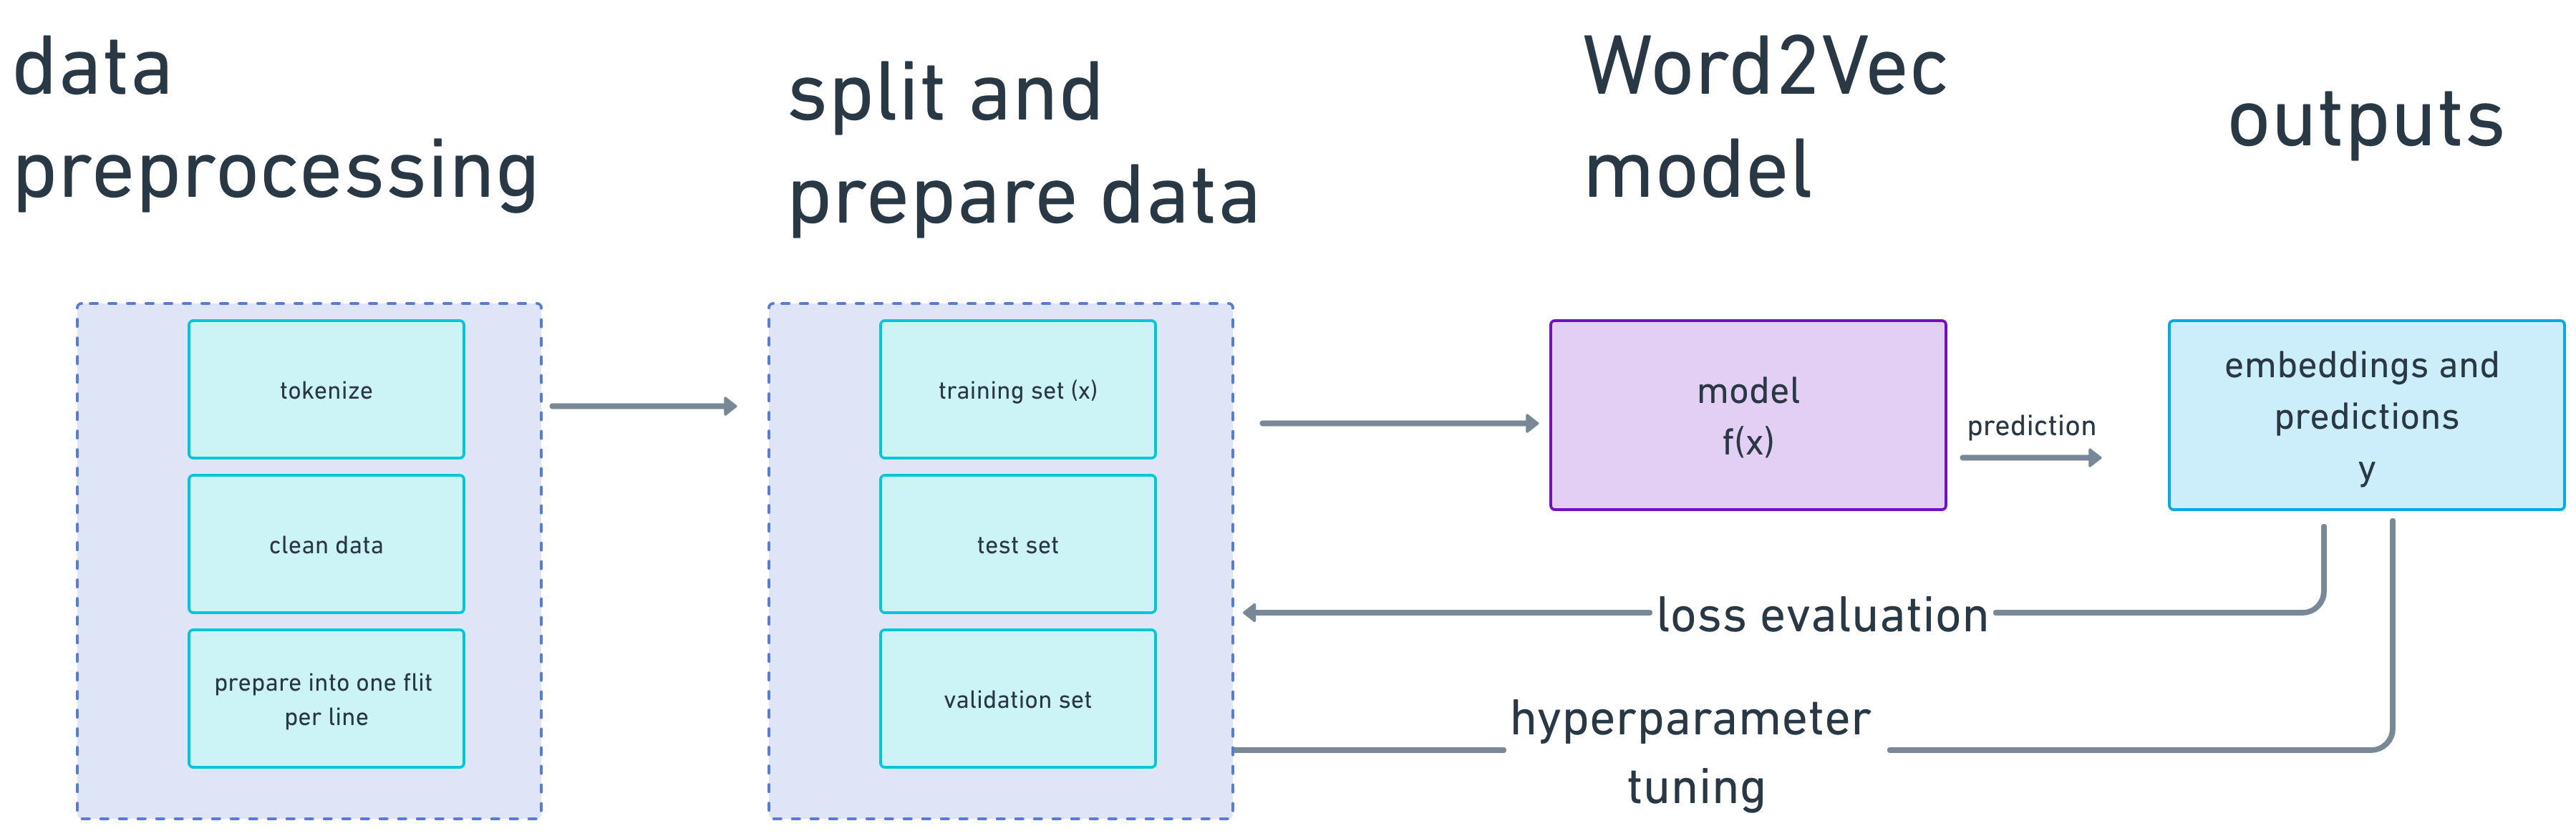
\includegraphics[width=\textwidth]
   	 {figures/word2vecmodel.png}}
   	 \caption{Steps for creating Word2Vec model}
      \end{figure}
	 
Let's start from our input data.  In this case, our corpus is all of the flits we've collected. We first need to process them as input into our model.

\begin{figure}[H]
\begin{minted}
[
frame=lines,
framesep=2mm,
baselinestretch=1.2,
fontsize=\footnotesize,
breaklines,
linenos
]{python3}
responses = ["Hold fast to dreams, for if dreams die, life is a broken-winged bird that cannot fly.", "No bird soars too high if he soars with his own wings.", "A bird does not sing because it has an answer, it sings because it has a song."]
\end{minted}
\caption{Our Word2Vec input dataset}
\end{figure}

Let's start with our input training data, which is our list of flits. To prepare input data for PyTorch, we can use the DataLoader or \hyperlink{https://pytorch.org/text/stable/vocab.html}{Vocab} classes, which splits our text into tokens and \textbf{tokenizes} --- or creates smaller, word-level representations of each sentence --- for processing.  For each line in the file, we generate tokens by splitting each line into single words, removing whitespace and punctuation, and lowercasing each individual word.

This kind of processing pipeline is extremely common in NLP and spending time to get this step right is extremely critical so that we get clean, correct input data. It typically includes \citep{naseem2021comprehensive}:

\begin{itemize}
  \item \textbf{Tokenization} - transforming a sentence or a word into its component character by splitting it
  \item \textbf{Removing noise} - Including URLs, punctuation, and anything else in the text  that is not relevant to the task at hand
  \item \textbf{Word segmentation} - Splitting our sentences into individual words
  \item \textbf{Correcting spelling mistakes}
\end{itemize}


\begin{figure}[H]
\begin{minted}
[
frame=lines,
framesep=2mm,
baselinestretch=1.2,
fontsize=\footnotesize,
linenos
]{python3}
class TextPreProcessor:
    def __init__(self) -> None:
   	 self.input_file = input_file

    def generate_tokens(self):
   	 with open(self.input_file, encoding="utf-8") as f:
   		 for line in f:
       		 line = line.replace("\\", "")
       		 yield line.strip().split()

    def build_vocab(self) -> Vocab:
   	 vocab = build_vocab_from_iterator(
   		 self.generate_tokens(), specials=["<unk>"], min_freq=100
   	 )
   	 return vocab
\end{minted}
\caption{Processing our input vocabulary and building a Vocabulary object from our dataset in PyTorch \href{https://github.com/veekaybee/viberary/tree/main/word2vec}{source}}
\end{figure}

Now that we have an input vocabulary object we can work with, the next step is to create one-hot encodings of each word to a numerical position, and each position back to a word, so that we can easily reference both our words and vectors. The goal is to be able to map back and forth when we do lookups and retrieval.

This occurs in the Embedding layer. Within the Embedding layer of PyTorch, we initialize an Embedding matrix based on the size we specify and size of our vocabulary, and the layer indexes the vocabulary into a dictionary for retrieval. The embedding layer is a lookup table\footnote{\href{https://pytorch.org/docs/stable/generated/torch.nn.Embedding.html}{Embedding Layer PyTorch documents}} that matches a word to the corresponding word vector on an index by index basis. Initially, we create our one-hot encoded word to term dictionary. Then, we create a mapping of each word to a dictionary entry and a dictionary entry to each word. This is known as \textbf{bijection}. In this way, the Embedding layer is like a one-hot encoded matrix, and allows us to perform lookups. The lookup values in this layer are initialized to a set of random weights, which we next pass onto the linear layer.

Embeddings resemble hash maps and also have their performance characteristics ($O(1)$ retrieval and insert time), which is why they can scale easily when other approaches cannot. In the embedding layer, Word2Vec where each value in the vector represents the word on a specific dimension, and more importantly, unlike many of the other methods, the value of each vector is in direct relationship to the other words in the input dataset.

\begin{figure}[H]
\begin{minted}
[
frame=lines,
framesep=2mm,
baselinestretch=1.2,
fontsize=\footnotesize,
linenos
]{python3}
class CBOW(torch.nn.Module):
    def __init__(self):  # we pass in vocab_size and embedding_dim as hyperparams
   	 super(CBOW, self).__init__()
   	 self.num_epochs = 3
   	 self.context_size = 2  # 2 words to the left, 2 words to the right
   	 self.embedding_dim = 100  # Size of your embedding vector
   	 self.learning_rate = 0.001
   	 self.device = torch.device('cuda' if torch.cuda.is_available() else 'cpu')

   	 self.vocab = TextPreProcessor().build_vocab()
   	 self.word_to_ix = self.vocab.get_stoi()
   	 self.ix_to_word = self.vocab.get_itos()
   	 self.vocab_list = list(self.vocab.get_stoi().keys())
   	 self.vocab_size = len(self.vocab)

   	 self.model = None

   	 # out: 1 x embedding_dim
   	 self.embeddings = nn.Embedding(
   		 self.vocab_size, self.embedding_dim
   	 )  # initialize an Embedding matrix based on our inputs
   	 self.linear1 = nn.Linear(self.embedding_dim, 128)
   	 self.activation_function1 = nn.ReLU()

   	 # out: 1 x vocab_size
   	 self.linear2 = nn.Linear(128, self.vocab_size)
   	 self.activation_function2 = nn.LogSoftmax(dim=-1)
\end{minted}
\caption{Word2Vec CBOW implementation in Pytorch. \href{https://github.com/veekaybee/viberary/tree/main/word2vec}{source}}
\end{figure}


Once we have our lookup values, we can process all our words. For CBOW, we take a single word and we pick a sliding window, in our case, two words before, and two words after, and try to infer what the actual word is. This is called the \textbf{context vector}, and in other cases, we'll see that it's called attention. For example, if we have the phrase "No bird [blank] too high", we're trying to predict that the answer is "soars" with a given softmax probability, aka ranked against other words. Once we have the context vector, we look at the loss --- the difference between the true word and the predicted word as ranked by probability --- and then we continue.

The way we train this model is through context windows. For each given word in the model, we create a sliding window that includes that word and 2 words before it, and 2 words after it.

We activate the linear layer with a \textbf{ReLu} activation function, which decides whether a given weight is important or not. In this case, ReLu squashes all the negative values we initialize our embeddings layer with down to zero since we can't have inverse word relationships, and we perform linear regression by learning the weights of the model of the relationship of the words. Then, for each batch we examine the \textbf{loss}, the difference between the real word and the word that we predicted should be there given the context window -  and we minimize it.

At the end of each epoch, or pass through the model, we pass the weights, or \textbf{backpropagate} them, back to the linear layer,and then again, update the weights of each word, based on the probability. The probability is calculated through a \textbf{softmax} function, which converts a vector of real numbers into a probability distribution - that is, each number in the vector, i.e. the value of the probability of each words, is in the interval between 0 and 1 and all of the word numbers add up to one.   The distance, as backpropogated to the embeddings table, should converge or shrink depending on the model understanding how close specific words are.

\begin{figure}[H]
\begin{minted}
[
frame=lines,
framesep=2mm,
baselinestretch=1.2,
fontsize=\footnotesize,
linenos
]{python3}

    def make_context_vector(self, context, word_to_ix) -> torch.LongTensor:
   	 """
   	 For each word in the vocab, find sliding windows of [-2,1,0,1,2] indexes
   	 relative to the position of the word
   	 :param vocab: list of words in the vocab
   	 :return: torch.LongTensor
   	 """
   	 idxs = [word_to_ix[w] for w in context]
   	 tensor = torch.LongTensor(idxs)


    def train_model(self):

   	 # Loss and optimizer
   	 self.model = CBOW().to(self.device)
   	 optimizer = optim.Adam(self.model.parameters(), lr=self.learning_rate)
   	 loss_function = nn.NLLLoss()

   	 logging.warning('Building training data')
   	 data = self.build_training_data()

   	 logging.warning('Starting forward pass')
   	 for epoch in tqdm(range(self.num_epochs)):
   		 # we start tracking how accurate our initial words are
   		 total_loss = 0

   		 # for the x, y in the training data:
   		 for context, target in data:
       		 context_vector = self.make_context_vector(context, self.word_to_ix)

       		 # we look at loss
       		 log_probs = self.model(context_vector)

       		 # compare loss
       		 total_loss += loss_function(
           		 log_probs, torch.tensor([self.word_to_ix[target]])
       		 )

   		 # optimize at the end of each epoch
   		 optimizer.zero_grad()
   		 total_loss.backward()
   		 optimizer.step()

   		 # Log out some metrics to see if loss decreases
   		 logging.warning("end of epoch {} | loss {:2.3f}".format(epoch, total_loss))

   	 torch.save(self.model.state_dict(), self.model_path)
   	 logging.warning(f'Save model to {self.model_path}')
\end{minted}
\caption Word2Vec CBOW implementation in PyTorch\\ \href{https://github.com/veekaybee/viberary/blob/main/src/notebooks/cbow.ipynb}{ see full implementation here}
\end{figure}

Once we've completed our iteration through our training set, we have learned a model that retrieves both the probability of a given word being the correct word, and the entire embedding space for our vocabulary.

\section{Modern Embeddings Approaches}

Word2Vec became one of the first neural network architectures to use the concept of embedding to create a fixed feature vocabulary. But neural networks as a whole were gaining popularity for natural language modeling because of several key factors. First, in the 1980s, researchers made advancements in using the technique of \textbf{backpropagation}  for training neural networks learning \citep{rumelhart1986learning}.  Backpropagation is how a model learns to converge by calculating the gradient of the loss function with respect to the weights of the neural network, using the \textbf{chain rule}, a concept from calculus which allows us to calculate the derivative of a function made up of multiple functions. This mechanism allows the model to understand when it's reached a global minimum for loss and picks the correct weights for the model parameters, but training models through gradient descent. Earlier approaches, such as the perceptron learning rule, tried to do this, but had limitations, such as being able to work only on simple layer architectures, took a long time to converge, and experienced \textbf{vanishing gradients}, which made it hard to effectively update the model's weights.  

These advances gave rise to the first kinds of multi-level neural networks, feed-forward neural networks. In 1998, a paper used backpropagation over multilayer perceptrons to correctly perform the task of recognizing handwritten digit images \citep{lecun1998gradient}, demonstrating a practical use-case practitioners and researchers could apply. This MNIST dataset is now one of the canonical "Hello World" examples of deep learning.

Second, in the 2000s, the rise of petabytes of aggregated log data resulted in the creation of large databases of multimodal input data scraped from the internet. This made it possible to conduct wide-ranging experiments to prove that neural networks work on large amounts of data. For example, ImageNet was developed by researchers at Stanford who wanted to focus on improving model performance by creating a gold set of neural network input data, the first step in processing. FeiFei Li assembled a team of students and paid gig workers from Amazon Turk to correctly label a set of 3.2 million images scraped from the internet and organized based on categories according to WordNet, a taxonomy put together by researchers in the 1970s \citep{russakovsky2015imagenet}.

Researchers saw the power of using standard datasets. In 2015, Alex Krizhevsky, in collaboration with Ilya Sutskever, who now works at OpenAI as one of the leading researchers behind the GPT series of models that form the basis of the current generative AI wave, submitted an entry to the ImageNet competition called AlexNet. This model was a convolutional neural network that outperformed many other methods. There were two things that were significant about AlexNet. The first was that it had eight stacked layers of weights and biases, which was unusual at the time. Today, 12-layer neural. networks like BERT and other transformers are completely normal, but at the time, more than two layers was revolutionary. The second was that it ran on GPUs, a new architectural concept at the time, since GPUs were used mostly for gaming.

Neural networks started to become popular as ways to generate representations of vocabularies. In particular, neural network architectures, such as  and \textbf{recurrent neural networks} (RNNs) and later \textbf{long short-term memory networks} (LSTMs) also emerged as ways to deal with textual data for all kinds of machine learning tasks from NLP to computer vision.


\subsection{Neural Networks}

Neural networks are extensions on traditional machine learning models, but they have a few critical special properties. Let's think back to our definition of a model when we formalized a machine learning problem. A model is a function with a set of learnable input parameters that takes some set of inputs and one set of tabular input features, and gives us an output. In traditional machine learning approaches, there is one set, or layer, of learnable parameters and  one model. If our data doesn't have complex interactions, our model can learn the feature space fairly easily and make accurate predictions.

However, when we start dealing with extremely large, implicit feature spaces, such as are present in text, audio, or video, we will not be able to derive specific features that wouldn't be obvious if we were manually creating them. A neural network, by stacking neurons, each of which represent some aspect of the model, can tease out these latent representations. Neural networks are extremely good at learning representations of data, with each level of the network transforming a learned representation of the level to a higher level until we get a clear picture of our data \citep{lecun2015deep}.

\subsubsection{Neural Network architectures}

We've already encountered our first neural network, Word2Vec, which seeks to understand relationships between words in our text that the words themselves would not tell us. Within the neural network space, there are several popular architectures:

\begin{formal}
\begin{itemize}
  \item Feed-forward networks that extract meaning from fixed-length inputs. Results of these model are not fed back into the model for iteration
  \item Convolutional neural nets (CNNs) - used mainly for image processing, which involves a convolutional layer made up of a filter that moves across an image to check for feature representations which are then multiplied via dot product with the filter to pull out specific features
  \item \textbf{recurrent neural networks}, which take a sequence of items and produce a vector that summarizes the sentence
\end{itemize}
\end{formal}

RNNs and CNNs are used mainly in feature extraction - they generally do not represent the entire modeling flow, but are fed later into feed-forward models that do the final work of classification, summarization, and more.

\begin{figure}[H]
\centering
\resizebox{.8\linewidth}{!}{%
\begin{forest}
  for tree={
    rectangle,
    align=center,
    rounded corners=3pt,
    grow=0,reversed, % tree direction
   	 parent anchor=east,child anchor=west, % edge anchors
   	 edge={line cap=round},outer sep=+1pt, % edge/node connection
  }
  [Neural Networks    [Feedforward 	 [Single-layer]
      [Multi-layer]
    ]
    [Recurrent 	 [Elman]
      [Jordan]
      [LSTM]
      [GRU]
    ]
    [Convolutional]
    [Autoencoder 	 [Vanilla]
      [Variational]
    ]
    [Generative Adversarial]
    [Radial Basis Function]
  ]
\end{forest}}
\caption{Types of Neural Networks}
\end{figure}


Neural networks are complex to build and manage for a number of reasons. First, they require extremely large corpuses of clean, well-labeled data to be optimized. They also require special GPU architectures for processing, and, as we'll see in the production section, they have their own metadata management and latency considerations. Finally, within the network itself, we need to complete a large amount of passes we need to do over the model object using batches of our training data to get it to converge. The number of feature matrices that we need to run calculations over\footnote{There is no good single resource for calculating the computational complexity of a neural network given that there are many wide-ranging architectures but   \href{https://lunalux.io/computational-complexity-of-neural-networks/}{this post} does a good job laying out the case that it's essentially $O(n^5)$}, and, consequently, the amount of data we have to keep in-memory through the lifecycle of the model ends up accumulating and requires a great deal of performance tuning.

These features made developing and running neural networks prohibitively expensive until the last fifteen years or so. First, the exponential increase in storage space provided by the growing size of commodity hardware both on-prem and in the cloud meant that we could now store that data for computation, and  the explosion of log data gave companies such as Google a lot of training data to work with.  Second,  the rise of the GPU as a tool that takes advantage of the neural network's ability to perform \textbf{embarrassingly parallel} computation --- a characteristic of computation when it's easy to separate steps out into ones that can be performed in parallel, such as word count for example. In a neural network, we can generally parallelize computation in any given number of ways, including at the level of a single neuron.  

While GPUs were initially used for working with computer graphics, in the early 2000s \citep{oancea2014gpgpu}, researchers discovered the potential to use them for general computation, and Nvidia made an enormous bet on this kind of computing by introducing CUDA, an API layer on top of GPUs. This in turn allowed for the creation and development of high-level popular deep learning frameworks like PyTorch and Tensorflow.

Neural networks could now be trained and experimented with at scale. To come back to a comparison to our previous approaches, when we calculate TF-IDF, we need to loop over each individual word and perform our computations over the entire dataset in sequence to arrive at a score in proportion to all other words, which means that our computational complexity will be $O(N D)$ \citep{cong2016novel}.  

However, with a neural network, we can either distribute the model training across different GPUs in a process known as \textbf{model parallelism}, or compute \textbf{batches} --- the size of the training data fed into the model and used in a training loop before its hyperparameters are updated in parallel and update at the end of each \textbf{minibatch}, which is known as \textbf{data parallelism.} \citep{shallue2018measuring}.


\subsection{Transformers}

Word2Vec is a feed-forward network. The model weights and information only flows from the encoding state, to the hidden embedding layer, to the output probability layer. There is no feedback between the second and third layers, which means that each given layer doesn't know anything about the state of the layers that follow it. It can't make inference suggestions longer than the context window. This works really well for machine learning problems where we're fine with a single, static vocabulary.

However, it doesn't work well on long ranges of text that require understanding words in context of each other. For example, over the course of a conversation, we might say, "I read that quote by Langston Hughes. I liked it, but didn't really read his later work," we understand that "it" refers to the quote, context from the previous sentence, and "his" refers to "Langston Hughes", mentioned two sentences ago.

One of the other limitations was that Word2Vec can't handle \textbf{out-of-vocabulary} words --- words that the model has not been trained on and needs to generalize to. This means that if our users search for a new trending term or we want to recommend a flit that was written after our model was trained, they won't see any relevant results from our model. \citep{di2021considerations}, unless the model is retrained frequently.

Another problem is that Word2Vec encounters context collapse around \textbf{polysemy} --- the coexistence of many possible meanings for the same phrase: for example, if you have "jail cell" and "cell phone" in the same sentence, it won't understand that the context of both words is different. Much of the work of NLP based in deep learning has been in understanding and retaining that context to propagate through the model and pull out semantic meaning.   

Different approaches were proposed to overcome these limitations. Researchers experimented with \textbf{recurrent neural networks}, RNNs. An RNN builds on traditional feed-forward networks, with the difference being that layers of the model give feedback to previous layers. This allows the model to keep memory of the context around words in a sentence.
 
\begin{figure}[H]
\centering
\begin{subfigure}[b]{0.4\linewidth}
\begin{tikzpicture}[
    shorten >=1pt,
    draw=black,
    node distance=2.5cm,line width=2pt,
    %
    input/.style={draw=black, circle, fill=black!30, minimum size=1cm},
    cell/.style={draw=black, rectangle, rounded corners=3mm, minimum width=3cm,
        		 minimum height=1.5cm, fill=black!10},
    %
    pre/.style={->},
    post/.style={<-}
    ]

    \node[cell]  (cell)   at (0,0)   	 {$Neuron$};
    \node[input,fill=cyan!40] (input)  at (0,-3) {$x_t$} edge[pre] (cell);
    \node[input,fill=violet!40,line width=2pt] (output) at (0,3) {$h_t$} edge[post] (cell);
    %
\end{tikzpicture}
\caption{Feedforward Neural Network}
\end{subfigure}
\begin{subfigure}[b]{0.4\linewidth}
\begin{tikzpicture}[
    shorten >=1pt,
    draw=black,
    node distance=2.5cm,line width=2pt,
    %
    input/.style={draw=black, circle, fill=black!30, minimum size=1cm},
    cell/.style={draw=black, rectangle, rounded corners=3mm, minimum width=3cm,
        		 minimum height=1.5cm, fill=black!10},
    %
    pre/.style={->},
    post/.style={<-}
    ]

    \node[cell]  (cell)   at (0,0)   	 {$Neuron$};
    \node[input,fill=cyan!40] (input)  at (0,-3) {$x_t$} edge[pre] (cell);
    \node[input,fill=violet!40,line width=2pt] (output) at (0,3) {$h_t$} edge[post] (cell);
    %
    \draw[rounded corners=5pt] (cell.east) -- (3,0) -- (3,2) -- (0.2,2);
    \draw[rounded corners=5pt,->] (-0.2,2) -- (-3,2) -- (-3,0) -- (cell.west);

\end{tikzpicture}
\caption{Recurrent Neural Network}
\end{subfigure}
\end{figure}

A problem with traditional RNNs was that because during backpropagation the weights had to be carried through to the previous layers of neurons, they experienced the problem of \textbf{vanishing gradients}. This occurs when we continuously take the derivative such that the partial derivative used in the chain rule during backpropagation approaches zero. Once we approach zero, the neural network assumes it has reached a local optimum and stops training, before convergence.

A very popular variation of an RNN that worked around this problem was the \textbf{long-short term memory network (LSTM)}, developed initially by Schmidhuber\footnote{If you read Schmidhuber, you will come to the understanding that everything in deep learning was developed initially by \href{https://people.idsia.ch/~juergen/deep-learning-miraculous-year-1990-1991.html}{Schmidhuber}} and brought to popularity for use in text applications speech recognition and image captioning \citep{karpathy_2015}.  Whereas our previous model takes only a vector at a time as input, RNNs operate on sequences of vectors using \textbf{GRUs}, which allows the network to control how much information is passed in for analysis. While LSTMs worked fairly well, they had their own limitations. Because they were architecturally complicated, they took much longer to train, and at a higher computational cost, because they couldn't be trained in parallel.

\subsubsection{Encoders/Decoders and Attention}
Two concepts allowed researchers to overcome computationally expensive issues with remembering long vectors for a larger \textbf{context window} than what was available in RNNs and Word2Vec before it: the \textbf{encoder/decoder architecture}, and the \textbf{attention mechanism}.

The encoder/decoder architecture is a neural network  architecture comprised of two neural networks, an encoder that takes the input vectors from our data and creates an embedding of a fixed length, and a decoder, also a neural network, which takes the embeddings encoded as input and generates a static set of outputs such as translated text or a text summary. In between the two types of layers is the \textbf{attention mechanism}, a way to hold the state of the entire input by continuously performing weighted matrix multiplications that highlight the relevance of specific terms in relation to each other in the vocabulary. We can think of attention as a very large, complex hash table that keeps track of the words in the text and how they map to different representations both in the input and the output.

\begin{figure}[H]
\centering
\tikzset
{
  myTrapezium/.pic =
  {
    \draw [fill=w_lightblue] (0,0) -- (0,\b) -- (\a,\c) -- (\a,-\c) -- (0,-\b) -- cycle ;
    \coordinate (-center) at (\a/2,0);
    \coordinate (-out) at (\a,0);
  },
  myArrows/.style=
  {
    line width=2mm,
    blue,
    -{Triangle[length=1.5mm,width=5mm]},
    shorten >=2pt,
    shorten <=2pt,
  }
}
    \def\a{3}  % width of trapezium
    \def\b{.9} % small height of trapezium
    \def\c{2}  % tall height of trapezium

\begin{tikzpicture}
[
  node distance=1mm, % space between drawn parts
  every node/.style={align=center},
]


  \node (middleThing)
  [
    draw,
    fill=w_lightblue,
    %minimum width=1cm,
    minimum height=2*\b cm,
    font=\tiny,
  ]
  {\begin{tabular}{r}-0.2 \\ -0.1 \\ 0.1 \\ 0.4 \\ -0.3 \\ 1.1\end{tabular}};
  \pic (right)[right=of middleThing.east] {myTrapezium} ;
  \pic (left)[left=of middleThing.west, rotate=180] {myTrapezium} ;
  \node at (right-center) {Decoder} ;
  \node at (left-center) {Encoder};
  \node at (right-center) {Decoder} ;

  \def\d{.9}
  \coordinate (u) at (\d,0);
  \draw [myArrows] (right-out) -- ++(u) node [anchor=west] {Translated\\text};
  \draw [myArrows] ($(left-out)-(u)$) node [anchor=east] {Input\\text} -- ++(u) ;

\end{tikzpicture}
\caption{The encoder/decoder architecture}
\end{figure}


\begin{figure}[H]
\begin{minted}
[
frame=lines,
framesep=2mm,
baselinestretch=1.2,
fontsize=\footnotesize,
linenos
]{python3}
class EncoderDecoder(nn.Module):
    """
       Defining the encoder/decoder steps
    """
    def __init__(self, encoder, decoder, src_embed, tgt_embed, generator):
   	 super(EncoderDecoder, self).__init__()
   	 self.encoder = encoder
   	 self.decoder = decoder
   	 self.src_embed = src_embed
   	 self.tgt_embed = tgt_embed
   	 self.generator = generator
  	 
    def forward(self, src, tgt, src_mask, tgt_mask):
   	 "Take in and process masked src and target sequences."
   	 return self.decode(self.encode(src, src_mask), src_mask,
                   		 tgt, tgt_mask)
    
    def encode(self, src, src_mask):
   	 return self.encoder(self.src_embed(src), src_mask)
    
    def decode(self, memory, src_mask, tgt, tgt_mask):
   	 return self.decoder(self.tgt_embed(tgt), memory, src_mask, tgt_mask)
  	 
class Generator(nn.Module):
    "Define standard linear + softmax generation step."
    def __init__(self, d_model, vocab):
   	 super(Generator, self).__init__()
   	 self.proj = nn.Linear(d_model, vocab)

    def forward(self, x):
   	 return F.log_softmax(self.proj(x), dim=-1)

\end{minted}
\caption{A typical encoder/decoder architecture  \href{http://nlp.seas.harvard.edu/2018/04/03/attention.html}{From the Annotated Transformer}}
\end{figure}


"Attention is All You Need" \citep{vaswani2017attention}, released in 2017,  combined both of these concepts into a single architecture. The paper immediately saw a great deal of success, and today Transformers are one of the de-facto models used for natural language tasks.

Based on the success of the original model, a great deal of variations on Transformer architectures have been released, followed by GPT and BERT in 2018, Distilbert, a smaller and more compact version of BERT in 2019, and GPT-3 in 2020\footnote{For a complete visual transformer timeline, check out \href{https://ai.v-gar.de/ml/transformer/timeline/}{this link}}.

\begin{figure}[H]
\centering
\begin{forest}
  for tree={
	parent anchor=south,
	child anchor=north,
	align=center,
	edge path={
  	\noexpand\path[\forestoption{edge}]
    	(!u.parent anchor) -- +(0,-5pt) -| (.child anchor)\forestoption{edge label};
	},
	font=\sffamily\small,
	edge={->}
  }
  [Transformer
	[GPT
  	[GPT-2]
  	[GPT-3
    	[DALL-E]
  	]
  	[GPT-4]
	]
	[BERT
  	[DistilBERT]
  	[RoBERTa]
	]
	[PaLM
	]
  ]
\end{forest}
\caption{Timeline of Transformer Models}
\end{figure}

Transformer architectures themselves are not new, but they contain all the concepts we've discussed so far: vectors, encodings, and hash maps. The goal of a transformer model is to take a piece of multimodal content, and learn the latent relationships by creating multiple views of groups of words in the input corpus (multiple context windows). The self-attention mechanism, implemented as scaled dot-product attention in the Transformer paper, creates different context windows of the data a number of times through the six encoder and six decoder layers. The output is the result of the specific machine learning task --- a translated sentence, a summarized paragraph -- and the next-to-last layer is the model's embeddings, which we can use for downstream work.

\begin{figure}[H]
\centering

\includegraphics[width=.9\textwidth]{figures/transformer_v.png}
\caption{View into transformer layers, inspired by multiple sources \href{https://lilianweng.github.io/posts/2018-06-24-attention/}{including this diagram } }
\end{figure}

The transformer model described in the paper takes a corpus of text as input\footnote{In theory you can use any modality for transformers without modifying the input other than to label the data with the given modality \citep{xu2023multimodal}, but the early work, such as machine translation, focuses on text, so we will as well}. We first transform our text to token embeddings by tokenizing and mapping every word or subword to an index. This is the same process as in Word2Vec: we simply assign each word to an element in a matrix. However, these alone will not help us with context, so, on top of this, we also learn a \textbf{positional embeddings} with the help of a sine or cosine function that is mapped and compressed into a matrix considering the position of all the other word in the vocabulary. The final output of this process is the positional vector or the word encoding.

Next, these positional vectors are passed in parallel to the model. Within the Transformer paper, the model consists of six layers that perform encoding and six that perform decoding. We start with the encoder layer, which consists of two sub-layers: the self-attention layer, and a feed-forward neural network. The self-attention layer is the key piece, which performs the process of learning the relationship of each term in relation to the other through \textbf{scaled dot-product attention.} We can think of self-attention in several ways: as a differentiable lookup table, or as a large lookup dictionary that contains both the terms and their positions, with the weights of each term in relationship to the other obtained from previous layers.

The scaled dot-product attention is  the product of three matrices: key, query, and value. These are initially all the same values that are outputs of previous layers - in the first pass through the model, they are initially all the same, initialized at random and adjusted at each step by gradient descent. For each embedding, we generate a weighted average value based on these learned attention weights. We calculate the dot product between query and key, and finally normalize the weights via softmax. \textbf{Multi-head attention} means that we perform the process of calculating the scaled dot product attention multiple times in parallel and concatenate the outcome into one vector.

\begin{equation}
Attention(Q, K, V) = softmax(\frac{QK^T}{\sqrt{d_k}})V
\end{equation}

What's great about scaled dot-product attention (and about all of the layers of the encoder) is that the work can be done in parallel across all the tokens in our codebase: we don't need to wait for one word to finish processing as we do in Word2Vec in order to process the next one, so the number of input steps remains the same, regardless of how big our vocabulary is.

The decoder piece differs slightly from the encoder. It starts with a different input dataset: in the transformer paper, it's the target language dataset we'd like to translate the text into.  So for example if we were translating our Flit from English to Italian, we'd expect to train on the Italian corpus. Otherwise, we perform all the same actions: we create indexed embeddings that we then convert into positional embeddings. We then feed the positional embeddings for the target text into a layer that has three parts: \textbf{masked multi-headed attention}, multiheaded attention, and a feed-forward neural network. The masked multi-headed attention component is just like self-attention, with one extra piece: the mask matrix introduced in this step acts as a filter to prevent the attention head from looking at future tokens, since the input vocabulary for the decoder are our "answers", I.e. what the translated text should be. The output from the masked multi-head self attention layer is passed to the encoder-decoder attention portion, which accepts the final input from the initial six encoder layers for the key and value, and uses the input from the previous decoder layer as the query, and then performs scaled dot-product over this. Each output is then fed into the feed forward layer, to a finalized set of embeddings.

Once we have the hidden state for each token, we can then attach the task head. In our case, this is prediction of what a word should be.  At each step of the process, the decoder looks at the previous steps and generates based on those steps so we form a complete sentence \citep{rush2018annotated}. We then get the predicted word, just like in Word2Vec.

Transformers were revolutionary for a number of reasons, because they solved several problems people had been working on:
\begin{itemize}
\item\textbf{Parallelization} - Each step in the model is parallelizable, meaning we don't need to wait to know the positional embedding of one word in order to work on another, since each embedding lookup matrix focuses attention on a specific word, with a lookup table of all other words in relationship to that word - each matrix for each word carries the context window of the entire input text.
\item\textbf{Vanishing gradients} - Previous models like RNNs can suffer from vanishing or exploding gradients, which means that the model reaches a local minimum before it's fully-trained, making it challenging to capture long-term dependencies. Transformers mitigate this problem by allowing direct connections between any two positions in the sequence, enabling information to flow more effectively during both forward and backward propagation.
\item\textbf{Self-attention} - The attention mechanism allows us to learn the context of an entire text that's longer than a 2 or 3-word sliding context window, allowing us to learn different words in different contexts and predict answers with more accuracy
\end{itemize}


\subsection{BERT}

\begin{figure}[H]
\centering{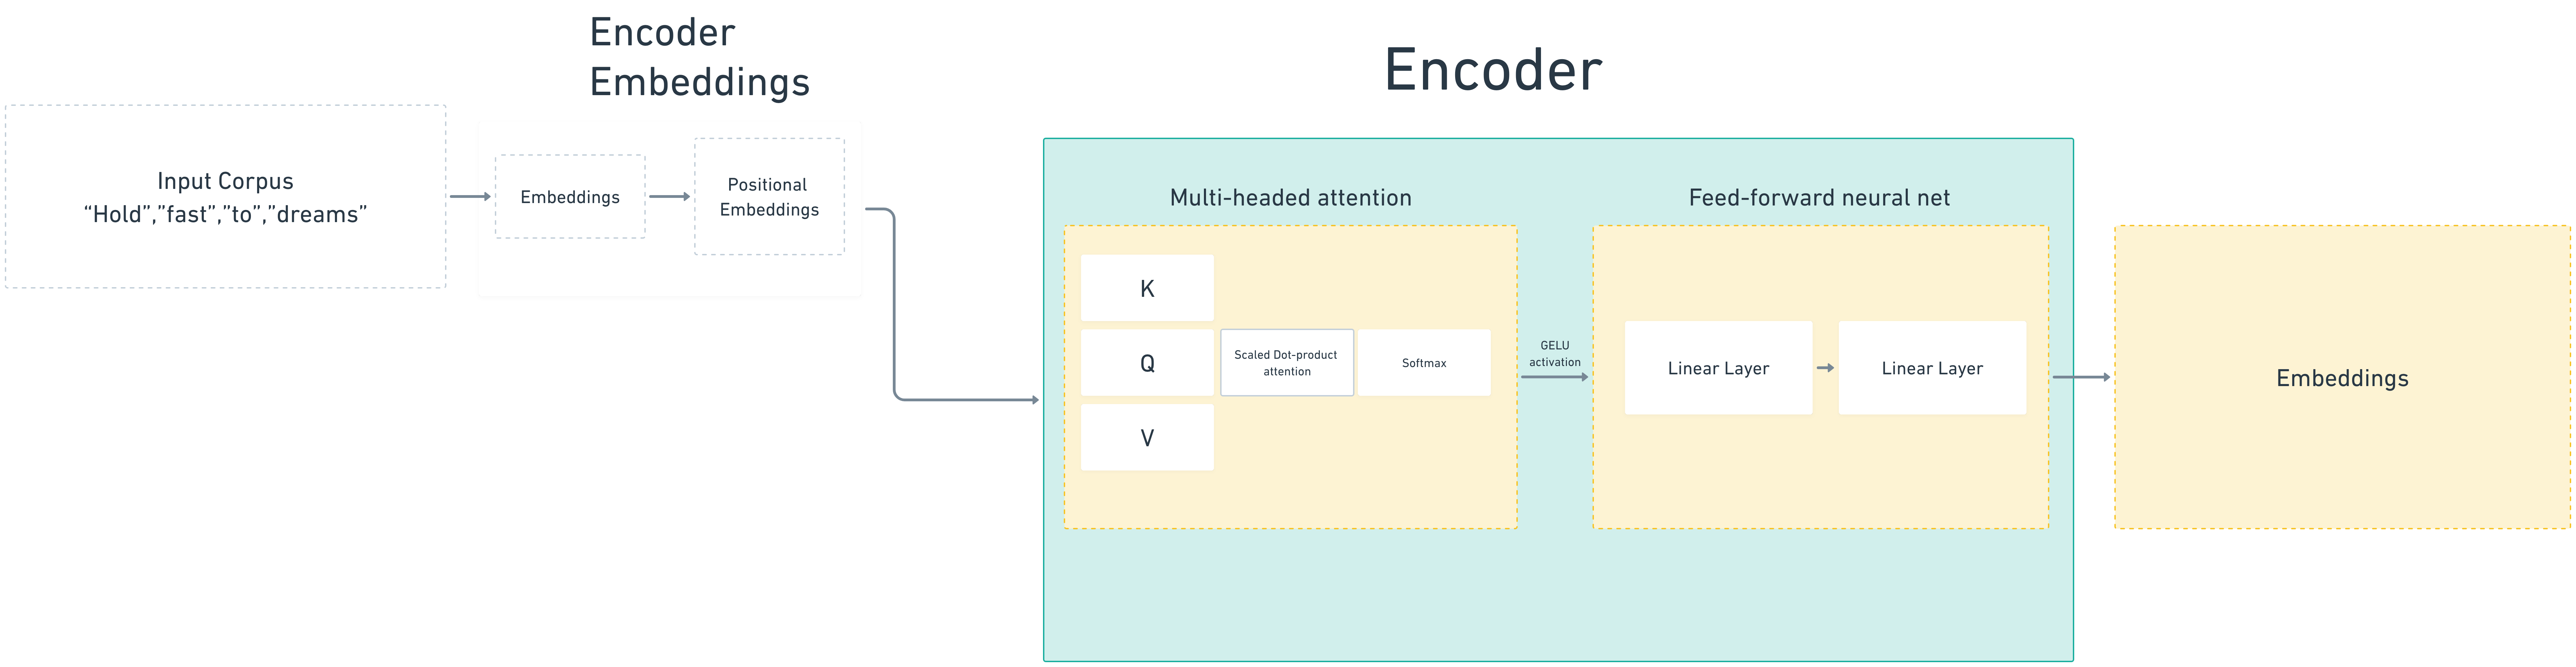
\includegraphics[width=.8\textwidth]{figures/encoder_only.png}}
\caption{Encoder-only architecture}
\end{figure}

After the explosive success of "Attention is All you Need", a variety of transformer architectures arose, research and implementation in this architecture exploded in deep learning. The next transformer architecture to be considered a significant step forward was \textbf{BERT}.
BERT stands for Bi-Directional Encoder and was released 2018 \citep{devlin2018bert}, based on a paper written by Google as a way to solve common natural language tasks like sentiment analysis, question-answering, and text summarization. BERT is a transformer model, also based on the attention mechanism, but its architecture is such that it only includes the encoder piece. Its most prominent usage is in Google Search, where it's the algorithm powering surfacing relevant search results. In the blog post they released on including BERT in search ranking in 2019, Google specifically discussed adding context to queries as a replacement for keyword-based methods as a reason they did this.\footnote{\href{https://blog.google/products/search/search-language-understanding-bert/}{BERT search announcement}}

BERT works as a \textbf{masked language model}. Masking is simply what we did when we implemented Word2Vec by removing words and building our context window. When we created our representations with Word2Vec, we only looked at sliding windows moving forward. The B in Bert is for bi-directional, which means it pays attention to words in both ways through scaled dot-product attention. BERT has 12 transformer layers. It starts by using \textbf{WordPiece}, an algorithm that segments words into subwords, into tokens. To train BERT, the goal is to predict a token given its context.

The output of BERT is latent representations of words and their context --- a set of embeddings. BERT is, essentially, an enormous parallelized Word2Vec that remembers longer context windows.  Given how flexible BERT is, it can be used for a number of tasks, from translation, to summarization, to autocomplete. Because it doesn't have a decoder component, it can't generate text, which paved the way for GPT models to pick up where BERT left off.


\subsection{GPT}
Around the same time that BERT was being developed, another transformer architecture, the GPT series, was being developed at OpenAI. GPT differs from BERT in that it encodes as well as decodes text from embeddings and therefore can be used for probabilistic inference.

The original, first GPT model was trained as a 12-layer, 12-headed transformer with only a decoder piece, based on data from Book Corpus. Subsequent versions built on this foundation to try and improve context understanding. The largest breakthrough was in GPT-4, which was trained with reinforcement learning from Human Feedback, a property which allows it to make inferences from text that feels much closer to what a human would write.

We've now reached the forefront of what's possible with embeddings in this paper. With the rise of generative methods and methods based on Reinforcement Learning with Human Feedback like OpenAI's ChatGPT, as well as the nascent open-source Llama, Alpaca, and other models,  anything written in this paper would already be impossibly out of date by the time it was published\footnote{There are already some studies about possible uses of LLMs for recommendations, including conversational recommender systems, but it's still very early days. For more information check out \href{https://blog.reachsumit.com/posts/2023/05/tuning-llm-for-recsys/}{this post}}.

\section{Embeddings in Production}

With the advent of Transformer models, and more importantly, BERT, generating representations of large, multimodal objects for use in all sorts of machine learning tasks suddenly became much easier, the representations became more accurate, and if the company had GPUs available, computations could now be computed with speed-up in parallel. Now that we understand what embeddings are, what should we do with them? After all, we're not doing this just as a math exercise. If there is one thing to take away from this entire text, it is this:

\begin{formal}
The final goal of all industrial machine learning (ML) projects is to develop ML products and rapidly bring them into production. \citep{kreuzberger2022machine}
\end{formal}

The model that is deployed is always better and more accurate than the model that is only ever a prototype. We've gone through the process of training embeddings end to end here, but there are several modalities for working with embeddings. We can:

\begin{itemize}
\item \textbf{Train our own embeddings model} - We can train BERT or some variation of BERT from scratch. BERT uses an enormous amount of training data, so this is not really advantageous to us, unless we want to better understand the internals and have access to a lot of GPUs.
\item \textbf{Use pretrained embeddings and fine-tune } - There are many variations on BERT models and they all Variations of BERT have been used to generate embeddings to use as downstream input into many recommender and information retrieval systems.  One of the largest gifts that the transformer architecture gives us is the ability to perform transfer learning. 

Before, when we learned embeddings in pre-transformer architectures, our representation of whatever dataset we had at hand was fixed --- we couldn't change the weights of the words in TF-IDF without regenerating an entire dataset. 
\end{itemize}

Now, we have the ability to treat the output of the layers of BERT as input into the next neural network layer of our own, custom model. In addition to transfer learning, there are also numerous more compact models for BERT, such as Distilbert and RoBERTA and for many of the larger models in places like the HuggingFace Model Hub\footnote{For a great writeup on the development of open-source machine learning deep learning, see  \href{https://colinraffel.com/blog/a-call-to-build-models-like-we-build-open-source-software.html}{"A Call to Build Models Like We Build Open-Source Software"}}.  

Armed with this knowledge, we can think of several use cases of embeddings, given their flexibility as a data structure.

\begin{formal}
\begin{itemize}
\item\textbf{Feeding them into another model} - For example, we can now perform collaborative filtering using both user and item embeddings that were learned from our data instead of coding the users and items themselves.
\item\textbf{Using them directly} - We can use item embeddings directly for content filtering - finding items that are closest to other items, a task recommendation shares with search. There are a host of algorithms used to perform vector similarity lookups by projecting items into our embedding space and performing similarity search using algorithms like faiss and HNSW.   
\end{itemize}
\end{formal}

\subsection{Embeddings in Practice}

Many companies are working with embeddings in all of these contexts today, across areas that span all aspects of information retrieval. Embeddings generated with deep learning models are being generated for use in wide and deep models for App Store recommendations at Google Play \citep{zhang2019deep}, dual embeddings for product complementary content recommendations at Overstock \citep{kvernadze2022two}, personalization of search results at Airbnb via real-time ranking \citep{grbovic2018real}, using embeddings for content understanding at Netflix \citep{dye_ekandham_saluja_rastogi_2020}, for understanding visual styles at Shutterstock \citep{gomez2022learning}, and many other examples.

\subsubsection{Pinterest}

One notable example is Pinterest. Pinterest as an application has a wide variety of content that needs to be personalized and classified for recommendation to users across multiple surfaces, particularly the Homefeed and shopping tab. The scale of generated content - 350 million monthly users and 2 billion items - Pins --- or cards with an image described by text --- necessitates a strong filtering and ranking policy.

To represent a user's interest and surface interesting content, Pinterest developed PinnerSage \citep{pal2020pinnersage}, which represents user interests through multiple 256-dimension embeddings that are clustered based on similarity and represented by \textbf{medioids} --- an item that is a representative of a center of a given interest cluster.

The foundation of this system is a set of embeddings developed through an algorithm called PinSage \citep{ying2018graph}. Pinsage generates embeddings using a Graph Convolutional neural network, which is a neural net that takes into account the graph structure of relationships between nodes in the network. The algorithm looks at the nearest neighbors of a pin and samples from nearby pins based on related neighborhood visits. The input is embeddings of a Pin: the image embeddings, and the text embeddings, and finds the nearest neighbors.

Pinsage embeddings are then passed to Pinnersage, which takes the pins the user has acted on for the past 90 days and clusters them. It computes the medioid and takes the top 3 medioids based on importance, and, given a user query that is a medioid, performs an approximate nearest neighbors search using HNSW to find the pins closest to the query in the embedding space.

\begin{figure}[H]
\centering{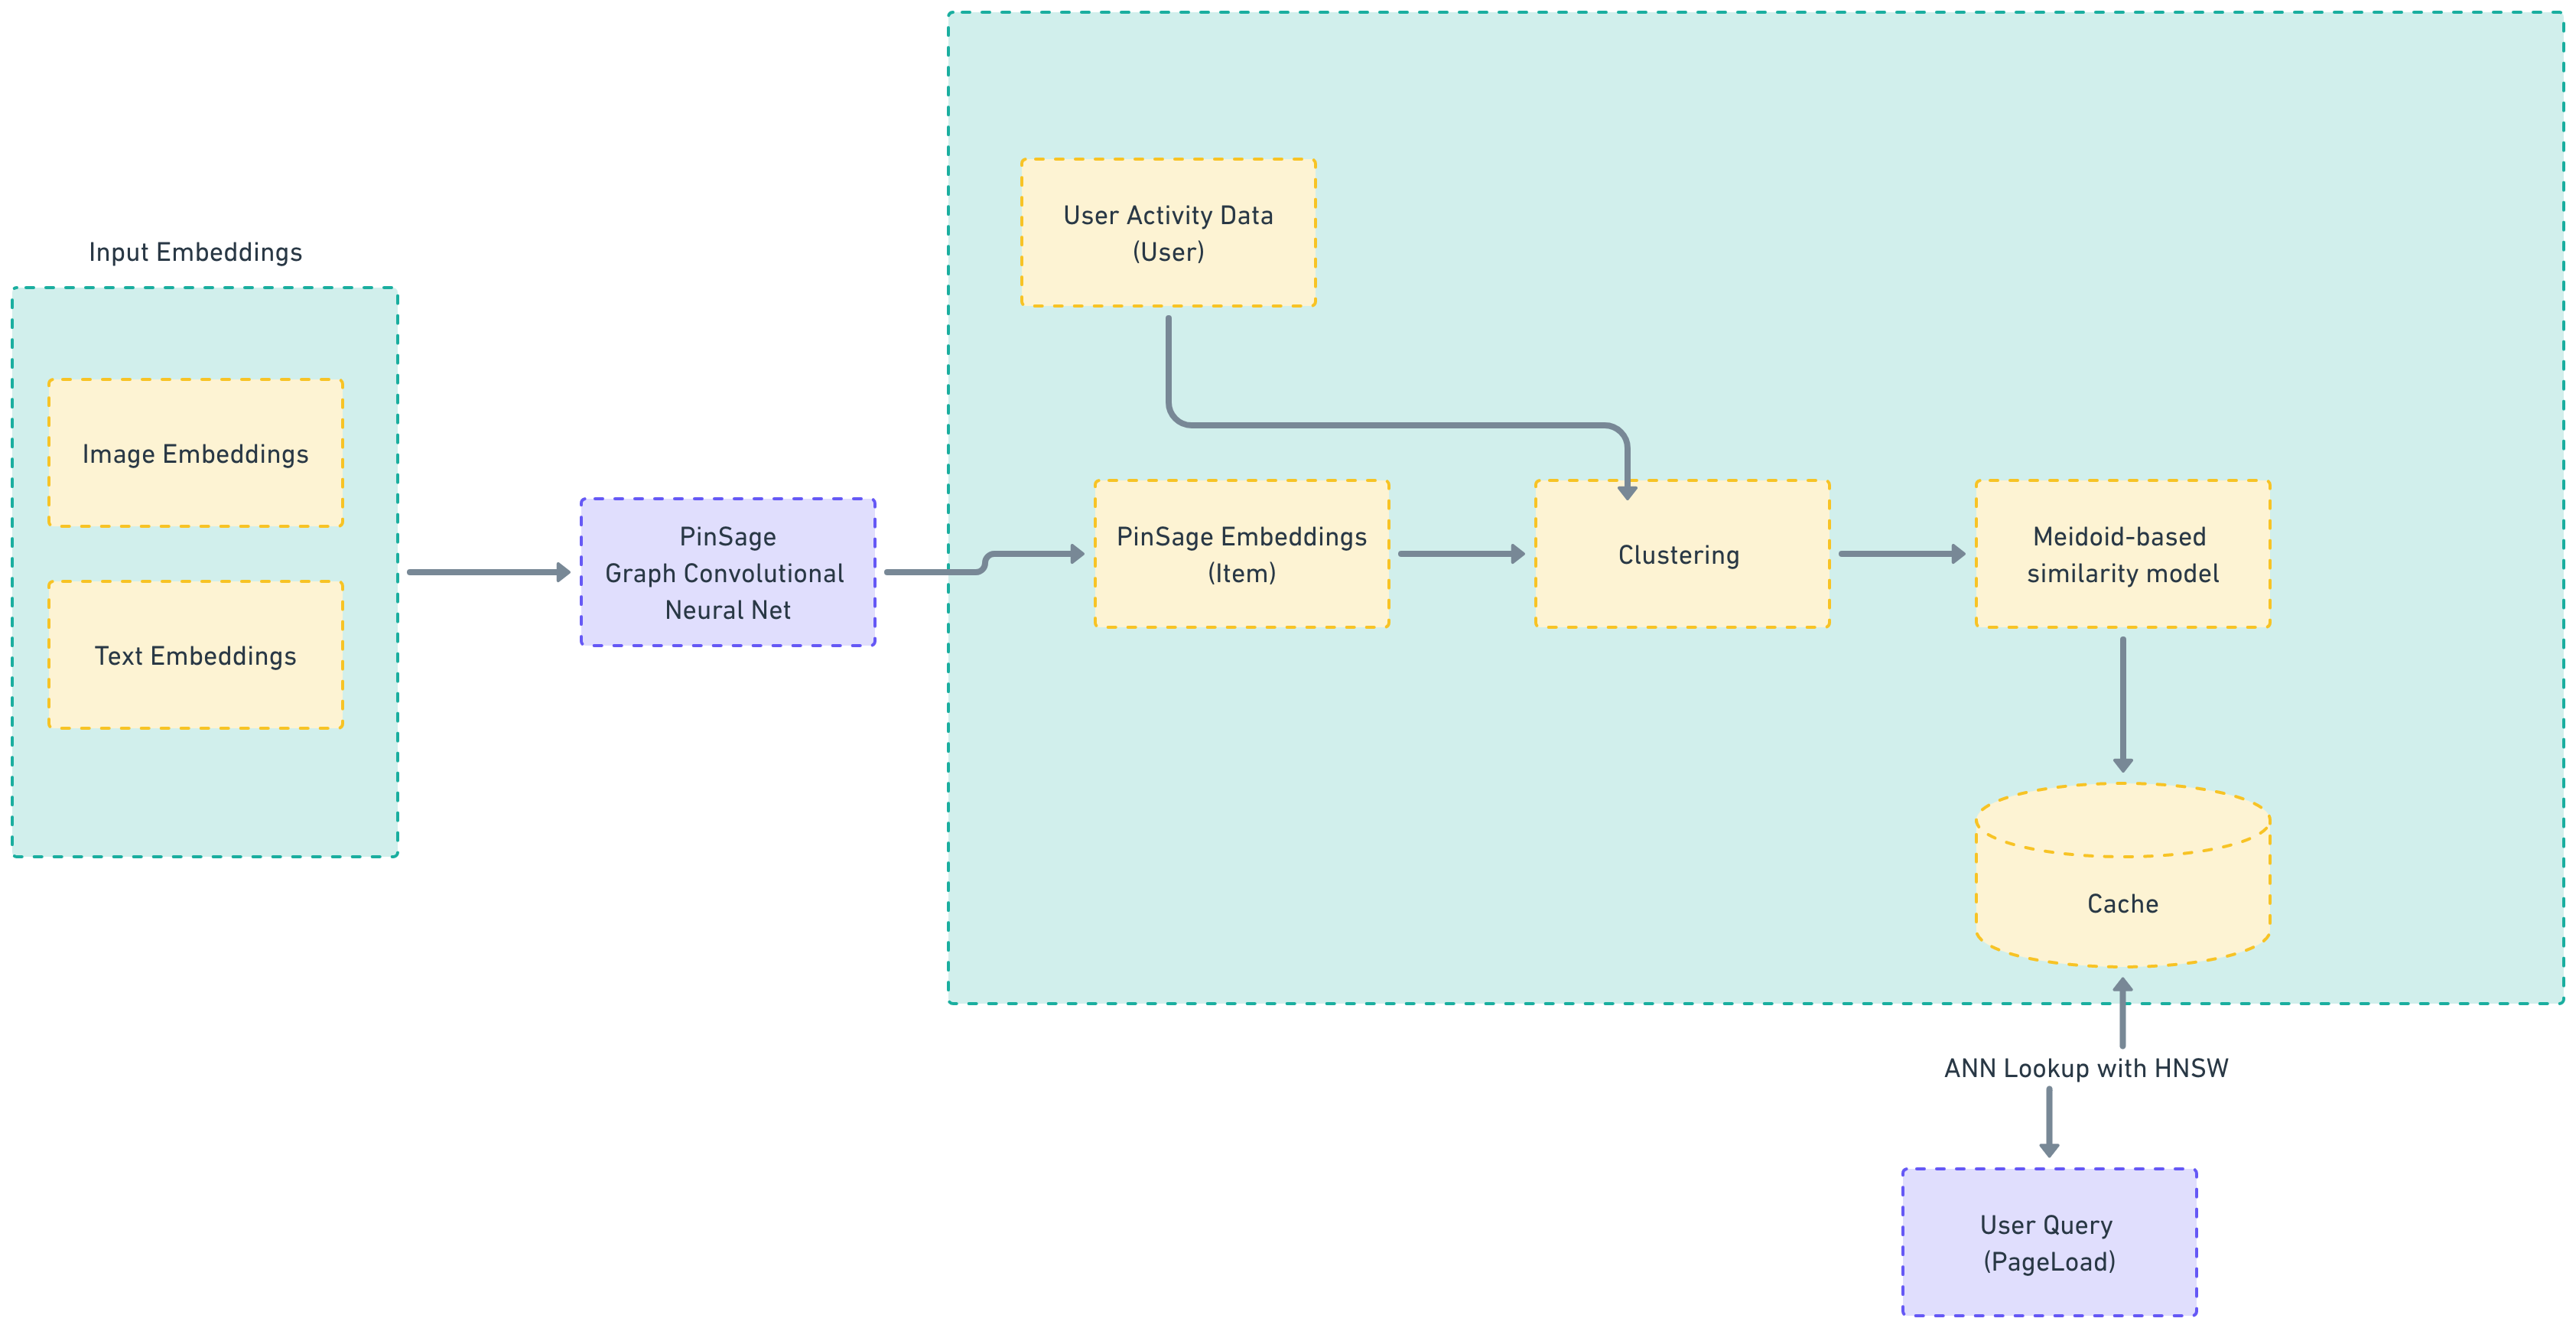
\includegraphics[width=.9\textwidth]{figures/pinnersage_model.png}}
\caption{Pinnersage and Pinsage embeddings-based similarity retrieval}
\end{figure}

\subsubsection{YouTube and Google Play Store}

\subsubsection*{YouTube}
\textbf{YouTube} was one of the first large companies to publicly share their work on embeddings used in the context of a production recommender system with "Deep Neural Networks for YouTube Recommendations."

YouTube has over 800 million pieces of content (videos) and ~2.6 billion active users that they'd like to recommend those videos to. The application needs to recommend existing content to users, while also generalizing to new content, which is uploaded frequently. They need to be able to serve these recommendations at \textbf{inference time} --- when the user loads a new page --- with low latency.

In this paper \citep{covington2016deep}, YouTube shares how they created a two-stage recommender system for videos based on two deep learning models. The machine learning task is to predict the correct next video to show the user at a given time in YouTube recommendations so that they click.  The final output is formulated as a classification problem: given a user's input features and the input features of a video, can we predict a class for the user that includes the predicted watch time for the user for a specific video with a specific probability.

\begin{figure}[H]
\centering{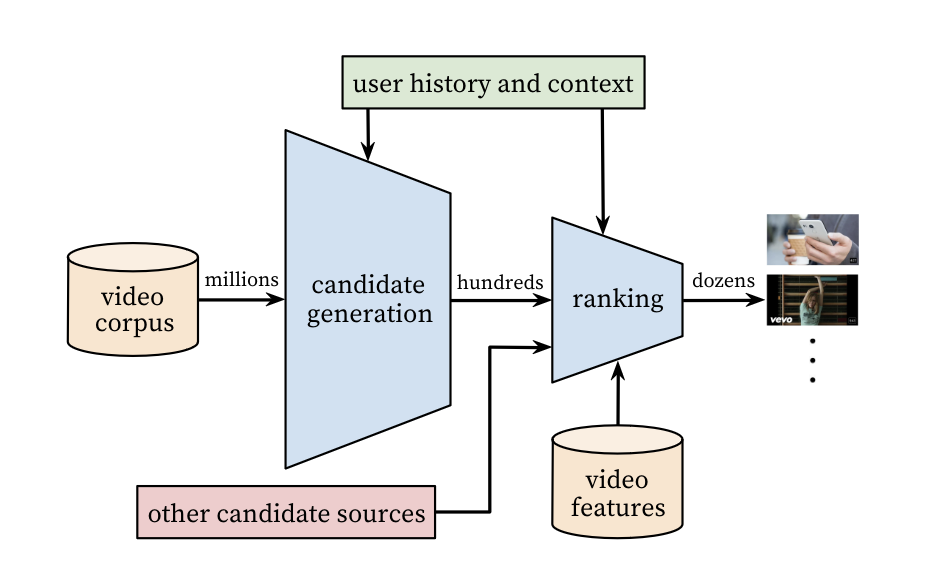
\includegraphics[width=.5\textwidth]{figures/youtube_recsys.png}}
\caption{YouTube's end-to-end video recommender system, including a candidate generator and ranker \citep{covington2016deep}}
\end{figure}

We set this task given a user, $U$ and \textbf{context} $C$\footnote{In recommender systems, we often think of \href{https://md.ekstrandom.net/blog/2015/10/search-and-recsys}{four relevant items} to formulate our recommender problem - user, item, context, and query. The context is usually the environment, for example the time of day or the geography of the user at inference time }

Given the size of the input corpus, we need to formulate the problem as a two-stage recommender: the first is the \textbf{candidate generator} that reduces the candidate video set to hundreds of items and a second model, similar in size and shape, called a \textbf{ranker} that ranks these hundreds of videos by the probability that the user will click on them and watch.

The candidate generator is a \textbf{softmax} deep learning model with several layers, all activated with \textbf{ReLU} activation functions --  rectified linear unit activation that outputs the input directly if positive; otherwise, it's zero.  The uses both embedded and tabular learning features, all of which are combined and



To build the model, we use two sets of embeddings as input data: one that's the user plus context as features, and a set of video items. The model has several hundreds of features, both tabular and embeddings-based. For the embeddings-based features, we include elements like:

\begin{itemize}
  \item User watch history - represented by a vector of sparse video ID elements mapped into a dense vector representation
  \item User's search history - Maps search term to video clicked from the search term, also in a sparse vector mapped into the same space as the user watch history
  \item User's geography, age, and gender - mapped as tabular features
  \item The number of previous impressions a video had, normalized per user over time
\end{itemize}


These are all combined into a single item embedding, and in the case of the user, a single embedding that's a blended map of all the user embedding features, and fed into the models' softmax layers, which compare the distance between the output of the softmax layer, i.e. the probability that the user will click on an item, and a set of ground truth items, i.e. a set of items that the user has already interacted with. The log probability of an item is the dot product of two n-dimensional vectors, i.e. the query and item embeddings.

We consider this an example of \textbf{Implicit} feedback - feedback the user did not explicitly give, such as a rating, but that we can capture in our log data.  Each class response, of which there are approximately a million, is given a probability as output.  

The DNN is a generalization of the matrix factorization model we discussed earlier.


\begin{figure}[H]
\centering{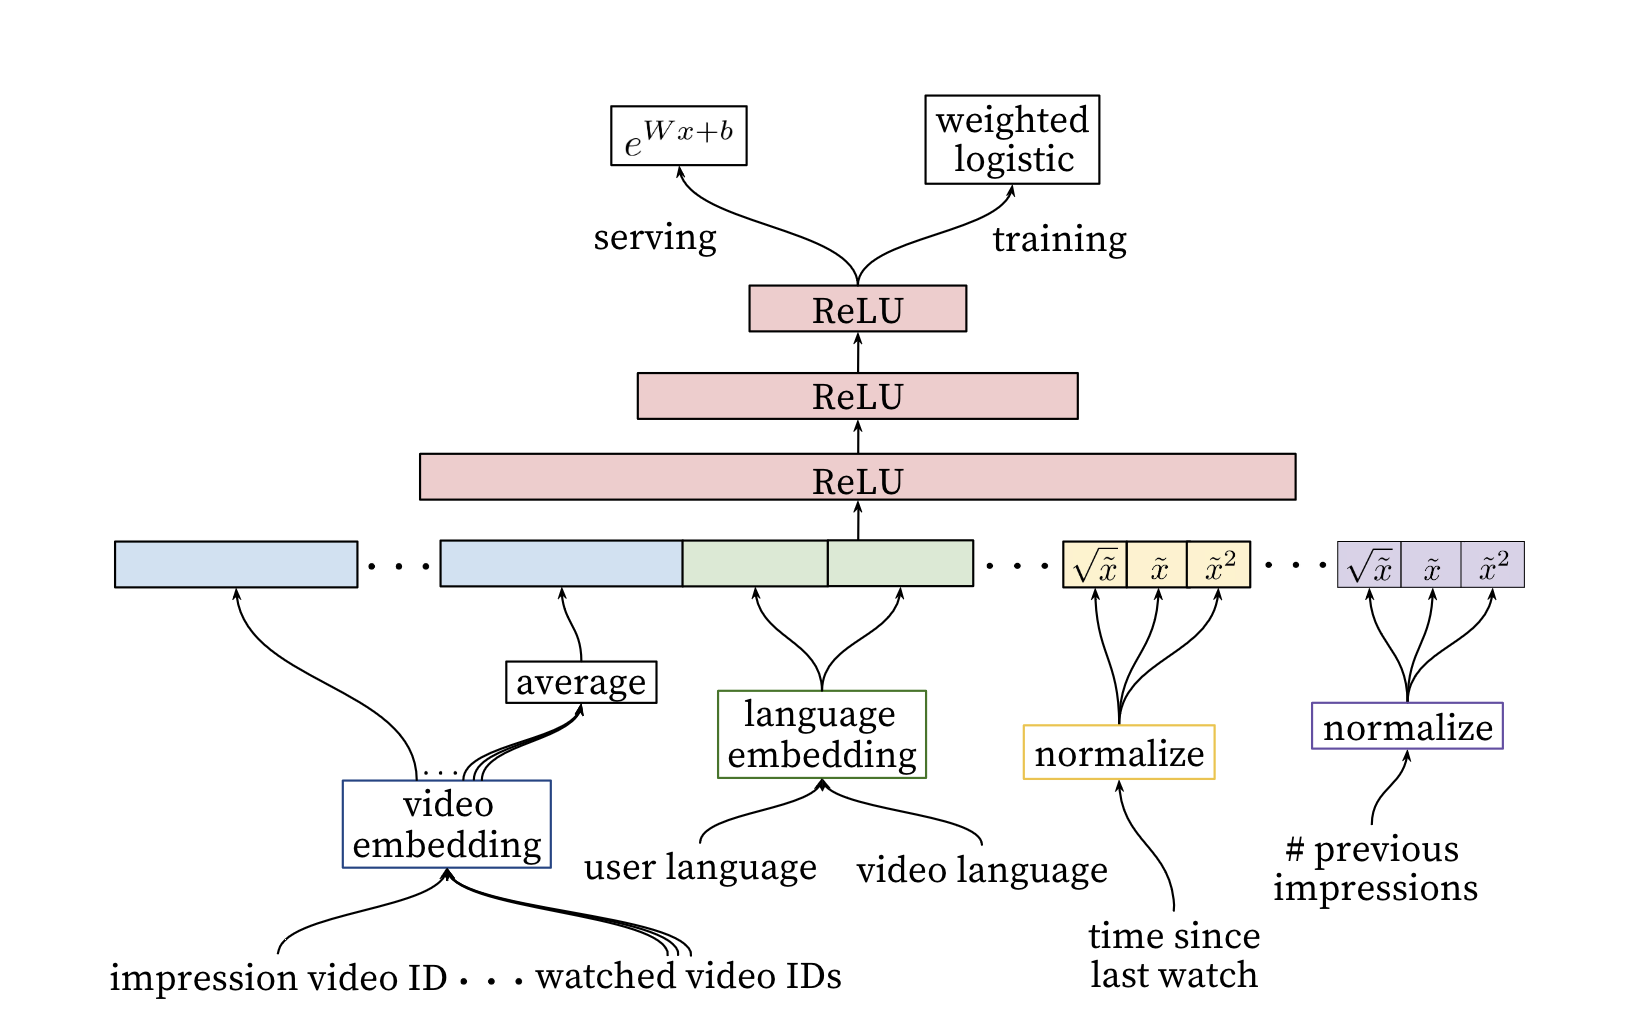
\includegraphics[width=\textwidth]{figures/youtube_model.png}}
\caption{YouTube's multi-step neural network model for video recommendations using input embeddings \citep{covington2016deep}}
\end{figure}

\subsubsection*{Google Play App Store}
Similar work, although with a different architecture, was done in the App Store in Google Play in "Wide and Deep Learning for Recommender Systems"  \citep{cheng2016wide}. This one crosses the search and recommendation space because it returns correct ranked and personalized app recommendations as the result of a search query.  The input is clickstream  data collected when a user visits the app store.


\begin{figure}[H]
\centering{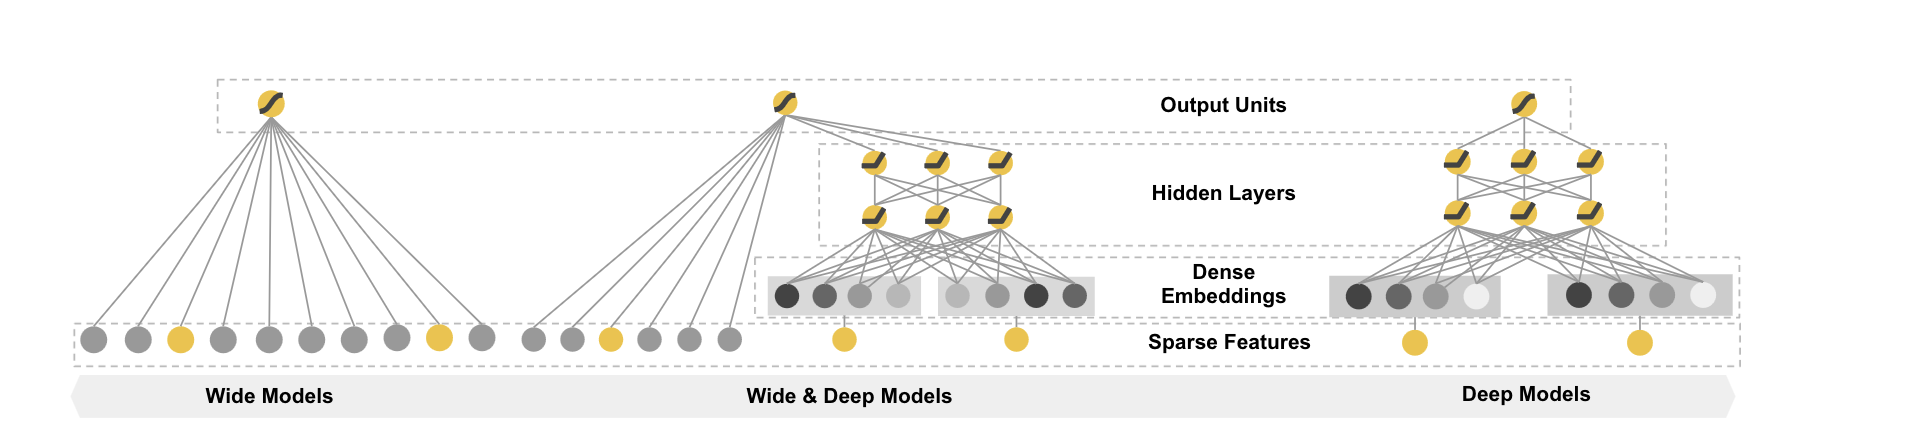
\includegraphics[width=\textwidth]{figures/wideanddeep_ml_arch.png}}
\caption{Wide and deep \citep{cheng2016wide}}
\end{figure}

The recommendations problem is formulated here as two jointly-trained models. The weights are shared and cross-propagated between the two models between epochs.

There are two problems when we try to build models that recommend items: \textbf{memorization} - the model needs to learn patterns by learning how items occur together given the historical data, and \textbf{generalization} - the model needs to be able to give new recommendations the user has not seen before that are still relevant to the user, improving recommendation diversity. Generally, one model alone cannot encompass both of these tradeoffs.  

Wide and deep is made up of two models that look to complement each other:

\begin{itemize}
  \item A \textbf{wide} model which uses traditional tabular features to improve the model's \textbf{memorization}. This is a general linear model trained on sparse, one-hot encoded features like \mintinline{python}{user_installed_app=netflix} across thousands of apps. Memorization works here by creating binary features that are combinations of features, such as \mintinline{python}{AND(user_installed_app=netflix, impression_app_pandora}, allowing us to see different combinations of co-occurrence in relationship to the target, i.e. likelihood to install app $Y$. However, this model cannot generalize if it gets a new value outside of the training data.
  \item A \textbf{deep} model that supports \textbf{generalization} across items that the model has not seen before, using a feed-forward neural network made up of categorical features that are translated to embeddings, such as user language, device class, and whether a given app has an impression. Each of these embeddings range from 0-100 in dimensionality. They are combined jointly into a concatenated embedding space with dense vectors in 1200 dimensions.  and initialized randomly. The embedding values are trained to minimize loss of the final function, which is a logistic loss function common to the deep and wide model.  
\begin{figure}[H]
\centering{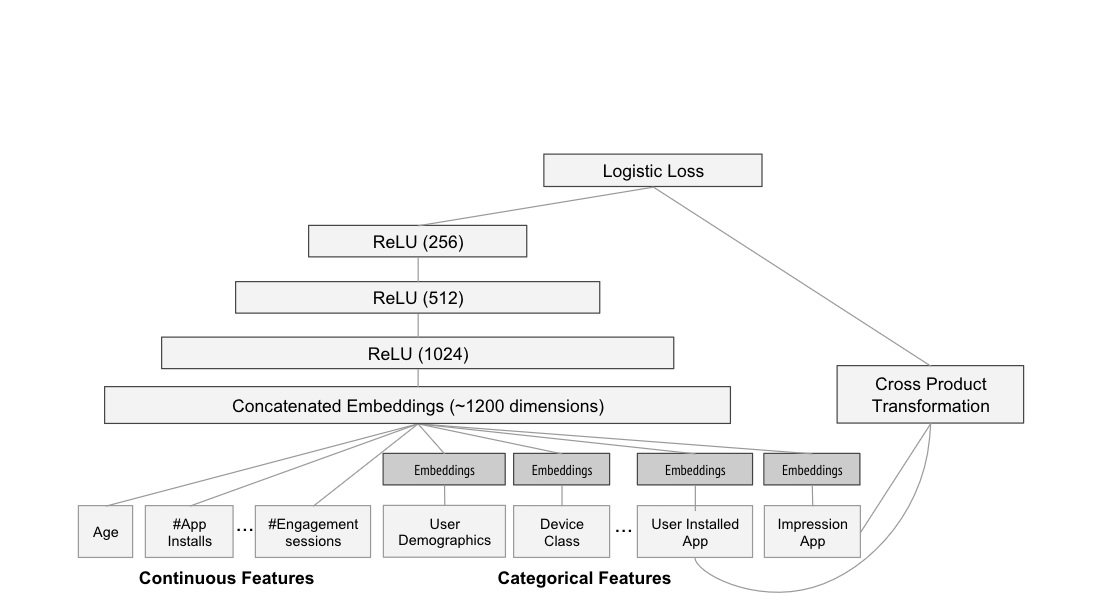
\includegraphics[width=1.1\textwidth]{figures/deepmodel.png}}
\caption{The deep part of the wide and deep model \citep{cheng2016wide}}
\end{figure}
\end{itemize}

The model is trained on 500 billion examples, and evaluated offline using AUC and online using app acquisition rate, the rate at which people download the app. Based on the paper, using this approach improved the app acquisition rate on the main landing page of the app store by 3.9 \% relative to the control group.


\subsubsection{Twitter}
At \textbf{Twitter},  pre-computed embeddings were a \href{https://blog.twitter.com/engineering/en_us/topics/insights/2018/embeddingsattwitter}{critical part} recommendations for many app surface areas including user onboarding topic interest prediction, recommended Tweets, home timeline construction, users to follow, and recommended ads.

Twitter had a number of embeddings-based models but we'll cover two projects here: Twice \citep{liu2022twice}, content embeddings for Tweets, which looks to find rich representations of Tweets that include both text and visual data for use in surfacing Tweets in the home timeline, Notifications and Topics. Twitter also developed TwHIN \citep{el2022twhin}, Twitter Heterogeneous Information Network, a set of graph-based embeddings \citep{el2022twhin}, developed for tasks like personalized ads rankings, account follow-recommendation, offensive content detection, and search ranking, based on nodes (such as users and advertisers) and edges that represent entity interactions.

\begin{figure}[H]
\centering{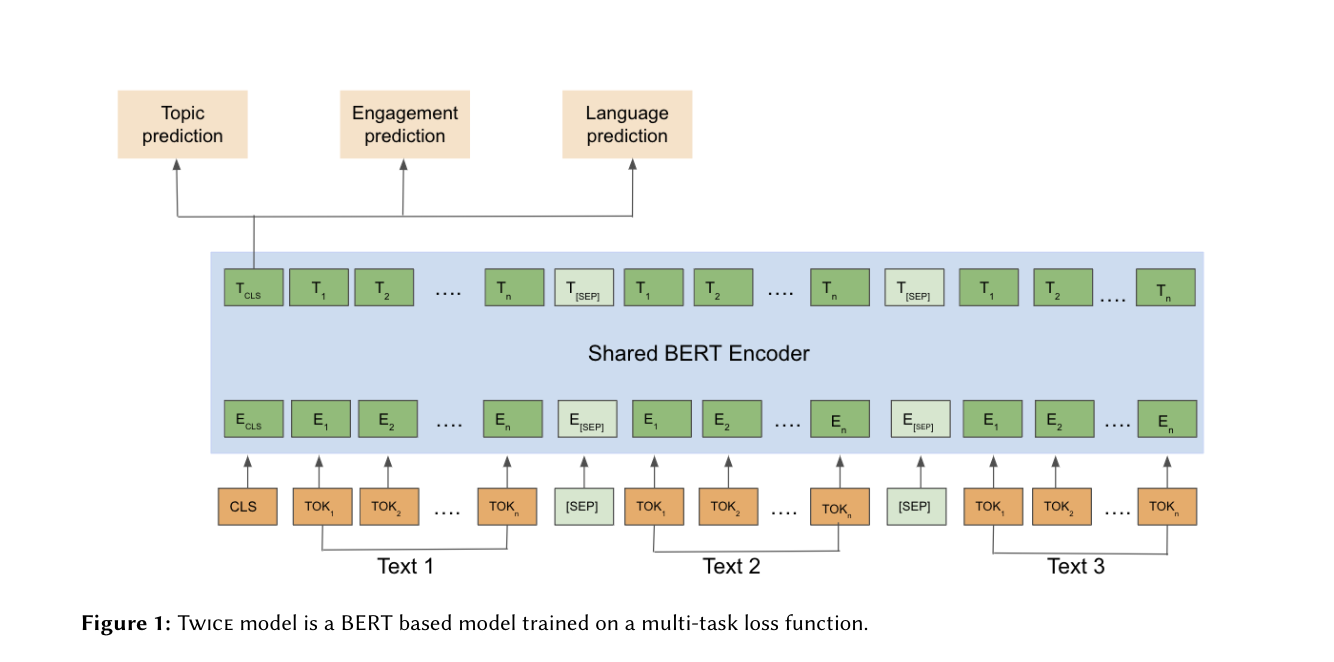
\includegraphics[width=.5\textwidth]{figures/twice.png}}
\caption{Twitter's Twice Embeddings, a trained BERT model \citep{liu2022twice}}
\end{figure}


Twice is a BERT model trained from scratch on an input corpus of 200 million Tweets that users engaged with sampled over 90 days and also includes associations to the users themselves. The objective of the model is to optimize on several tasks: topic prediction (aka the topic associated with a Tweet, of which there could be multiple), engagement prediction (the likelihood a user is to engage with a Tweet), and language prediction to cluster Tweets of the same language to be clustered closer together.


TwHIN, rather than just focusing on Tweet content, considers all entities in Twitter's environment (Tweets, users, advertiser entities) as belong together in a joint embedding space graph.

Joint embedding is performed by using data from user-Tweet engagement, advertising, and following data, to create multi-model embeddings. TWHin is used for candidate generation. The candidate generator finds users to follow or Tweets to engage with an HNSW or Faiss to retrieve candidate items. TWHin embeddings are then used to query candidate items and increase diversity in the candidate pool.

\begin{figure}[H]
\centering{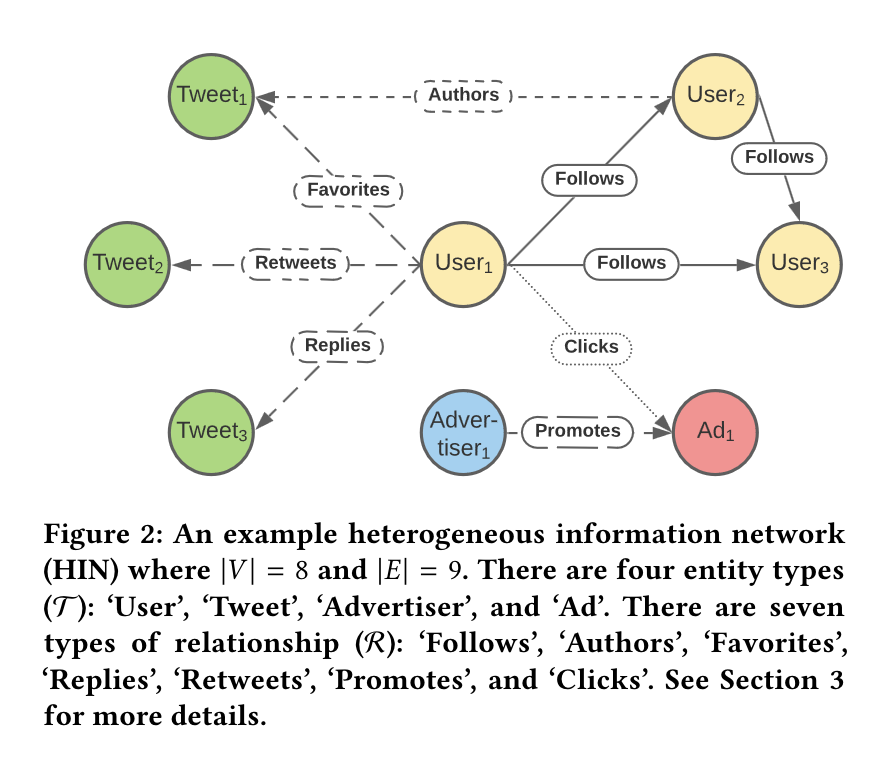
\includegraphics[width=.7\textwidth]{figures/twhin.png}}
\caption{Twitter's model of the app's heterogeneous information network \citep{el2022twhin}}
\end{figure}


\subsubsection*{Embeddings at Flutter}

Once we synthesize enough of these architectures, we see some patterns start to emerge that we can think about adapting for developing our relevant recommendation system at Flutter.

First, we need a great deal of input data to make accurate predictions from, and that data should have information about either explicit, or, more likely, implicit data like user clicks and purchases so that we can construct our model of user preferences. The reason we need a lot of data is two-fold. First, neural networks are data-hungry and require a large amount of training data to correctly infer relationships in comparison to traditional models. Second, large data requires a large pipeline.  

If we don't have a lot of data, a simpler model will work well-enough, so we need to make sure we are actually at the scale where embeddings and neural networks help our business problem. It's likely the case that we can start much simpler. And in fact, a recent paper by one of the original researchers who developed factorization machines, an important approach in recommendations, argues that simple dot products found as the result of matrix factorization outperform neural networks \citep{rendle2020neural}.  Second, in order to get good embeddings, we will need to spend a great deal of time cleaning and processing data and creating features, as we did in the YouTube paper, so the outcome has to be worth the time spent.

Second, we need to be able to understand the latent relationship between users and items they've interacted with. In traditional recommenders, we could use TF-IDF to find the weighted word features as part of a particular flit and compare across documents, as long as our corpus doesn't grow too large. In more advanced recommendation systems, we could perform this same task by looking at either naive association rules, or framing recommendation as an interaction-based collaborative filtering problem not unlike Word2Vec to generate latent features, aka embeddings, of our users and items. In fact, this is exactly what Levy and Goldberg argued in "Neural Word Embedding as Implicit Matrix Factorization"  \citep{levy2014neural}. They looked at the skipgram implementation of Word2Vec and found that implicitly it factors a word-context matrix.

We could alternatively still use tabular features as input into our collaborative filtering problem but use a neural network \citep{he2017neural} instead of simple dot product to converge on the correct relationships and the downstream ranking for the model.

Given our new knowledge about how embeddings and recommender systems work, we can now incorporate embeddings into the recommendations we serve for flits at Flutter.  If we want to recommend relevant content, we might do it in a number of different ways, depending on our business requirements.  In our corpus, we have hundreds of millions of messages that we need to filter down to hundreds to show the user. So we can start with a baseline of Word2Vec or similar and move on to any of the BERT or other neural network approaches to developing model input features, vector similarity search, and ranking, through the power of embeddings.

Embeddings are endlessly flexible and endlessly useful, and can empower and improve the performance of our multimodal machine learning workflows. However, as we just saw, there are some things to keep in mind if we do decide to use them.

\subsection{Embeddings as an Engineering Problem}

In general, machine learning workflows add an enormous amount of complexity and overhead to our engineering systems, for a number of reasons \citep{sculley2014machine}. First, they blend data that then needs to be monitored for drift downstream. Second, they are non-deterministic in their outputs, which means they need to be tracked extremely carefully as artifacts, since we generally don't version-control data. Third, they result in processing pipeline jungles.


\begin{quote}
As a special case of glue code, pipeline jungles often appear in data preparation. These can evolve organically, as new signals are identified and new information sources added. Without care, the resulting system for preparing data in an ML-friendly format may become a jungle of scrapes, joins, and sampling steps, often with intermediate files output.
\end{quote}

As we can see from several system diagrams, including PinnerSage and the Wide and Deep Model, \href{https://amatriain.net/blog/RecsysArchitectures}{recommender systems in production utilizing embeddings have} many moving components.


\begin{figure}[H]
  \centering
  \begin{minipage}[b]{0.4\textwidth}
	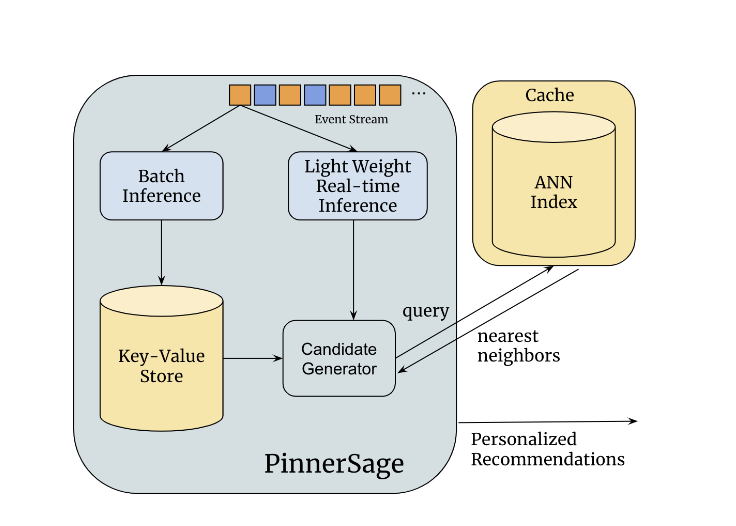
\includegraphics[width=\textwidth]{figures/pinnersage.png}
	\caption{PinnerSage model architecture \citep{pal2020pinnersage}}
  \end{minipage}
  \hfill
  \begin{minipage}[b]{0.4\textwidth}
	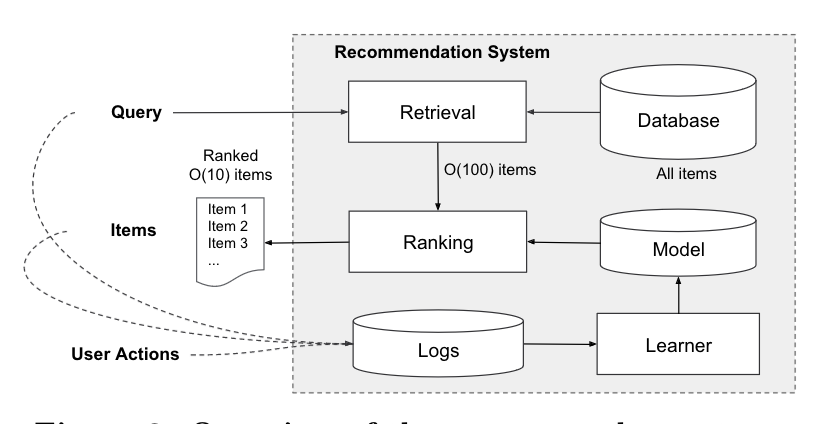
\includegraphics[width=\textwidth]{figures/wideanddeep_arch.png}
	\caption{Wide and Deep model architecture \citep{cheng2016wide}}
  \end{minipage}
\end{figure}

You may recall that we discussed the simple stages of a recommender system in this diagram.

\begin{figure}[H]
\centering
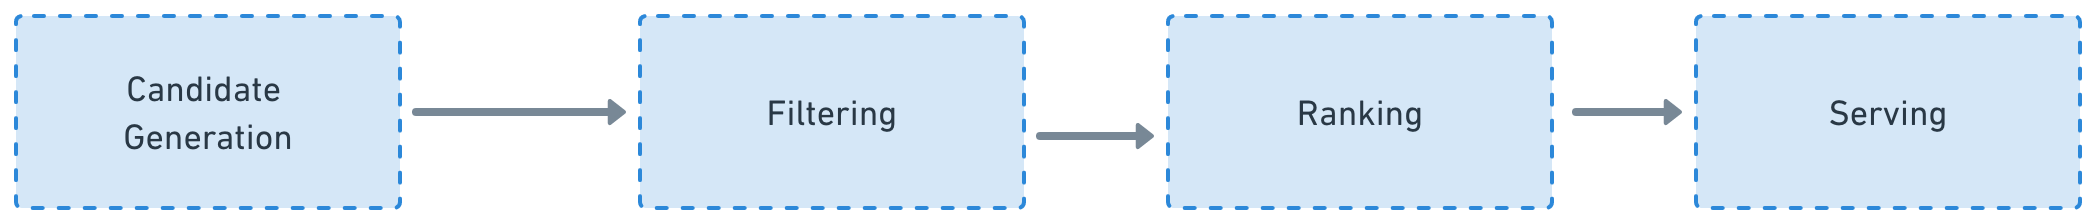
\includegraphics[width=\textwidth]{figures/recsys.png}
\caption{Generic system processing embeddings in context}
\end{figure}

Given all of our production-level requirements for a successful recommendation system, our actual production system generally looks more like this:

\begin{formal}
\begin{itemize}
  \item Generating embeddings
  \item Storing embeddings
  \item Embedding feature engineering and iteration
  \item Artifact retrieval
  \item updating embeddings
  \item versioning embeddings and data drift
  \item Inference and latency
  \item Online (A/B test) and offline (metric sweep) model evaluation
\end{itemize}
\end{formal}

Given all of our concern space, the diagram of any given production system would look more like this

\begin{figure}[H]
\centering
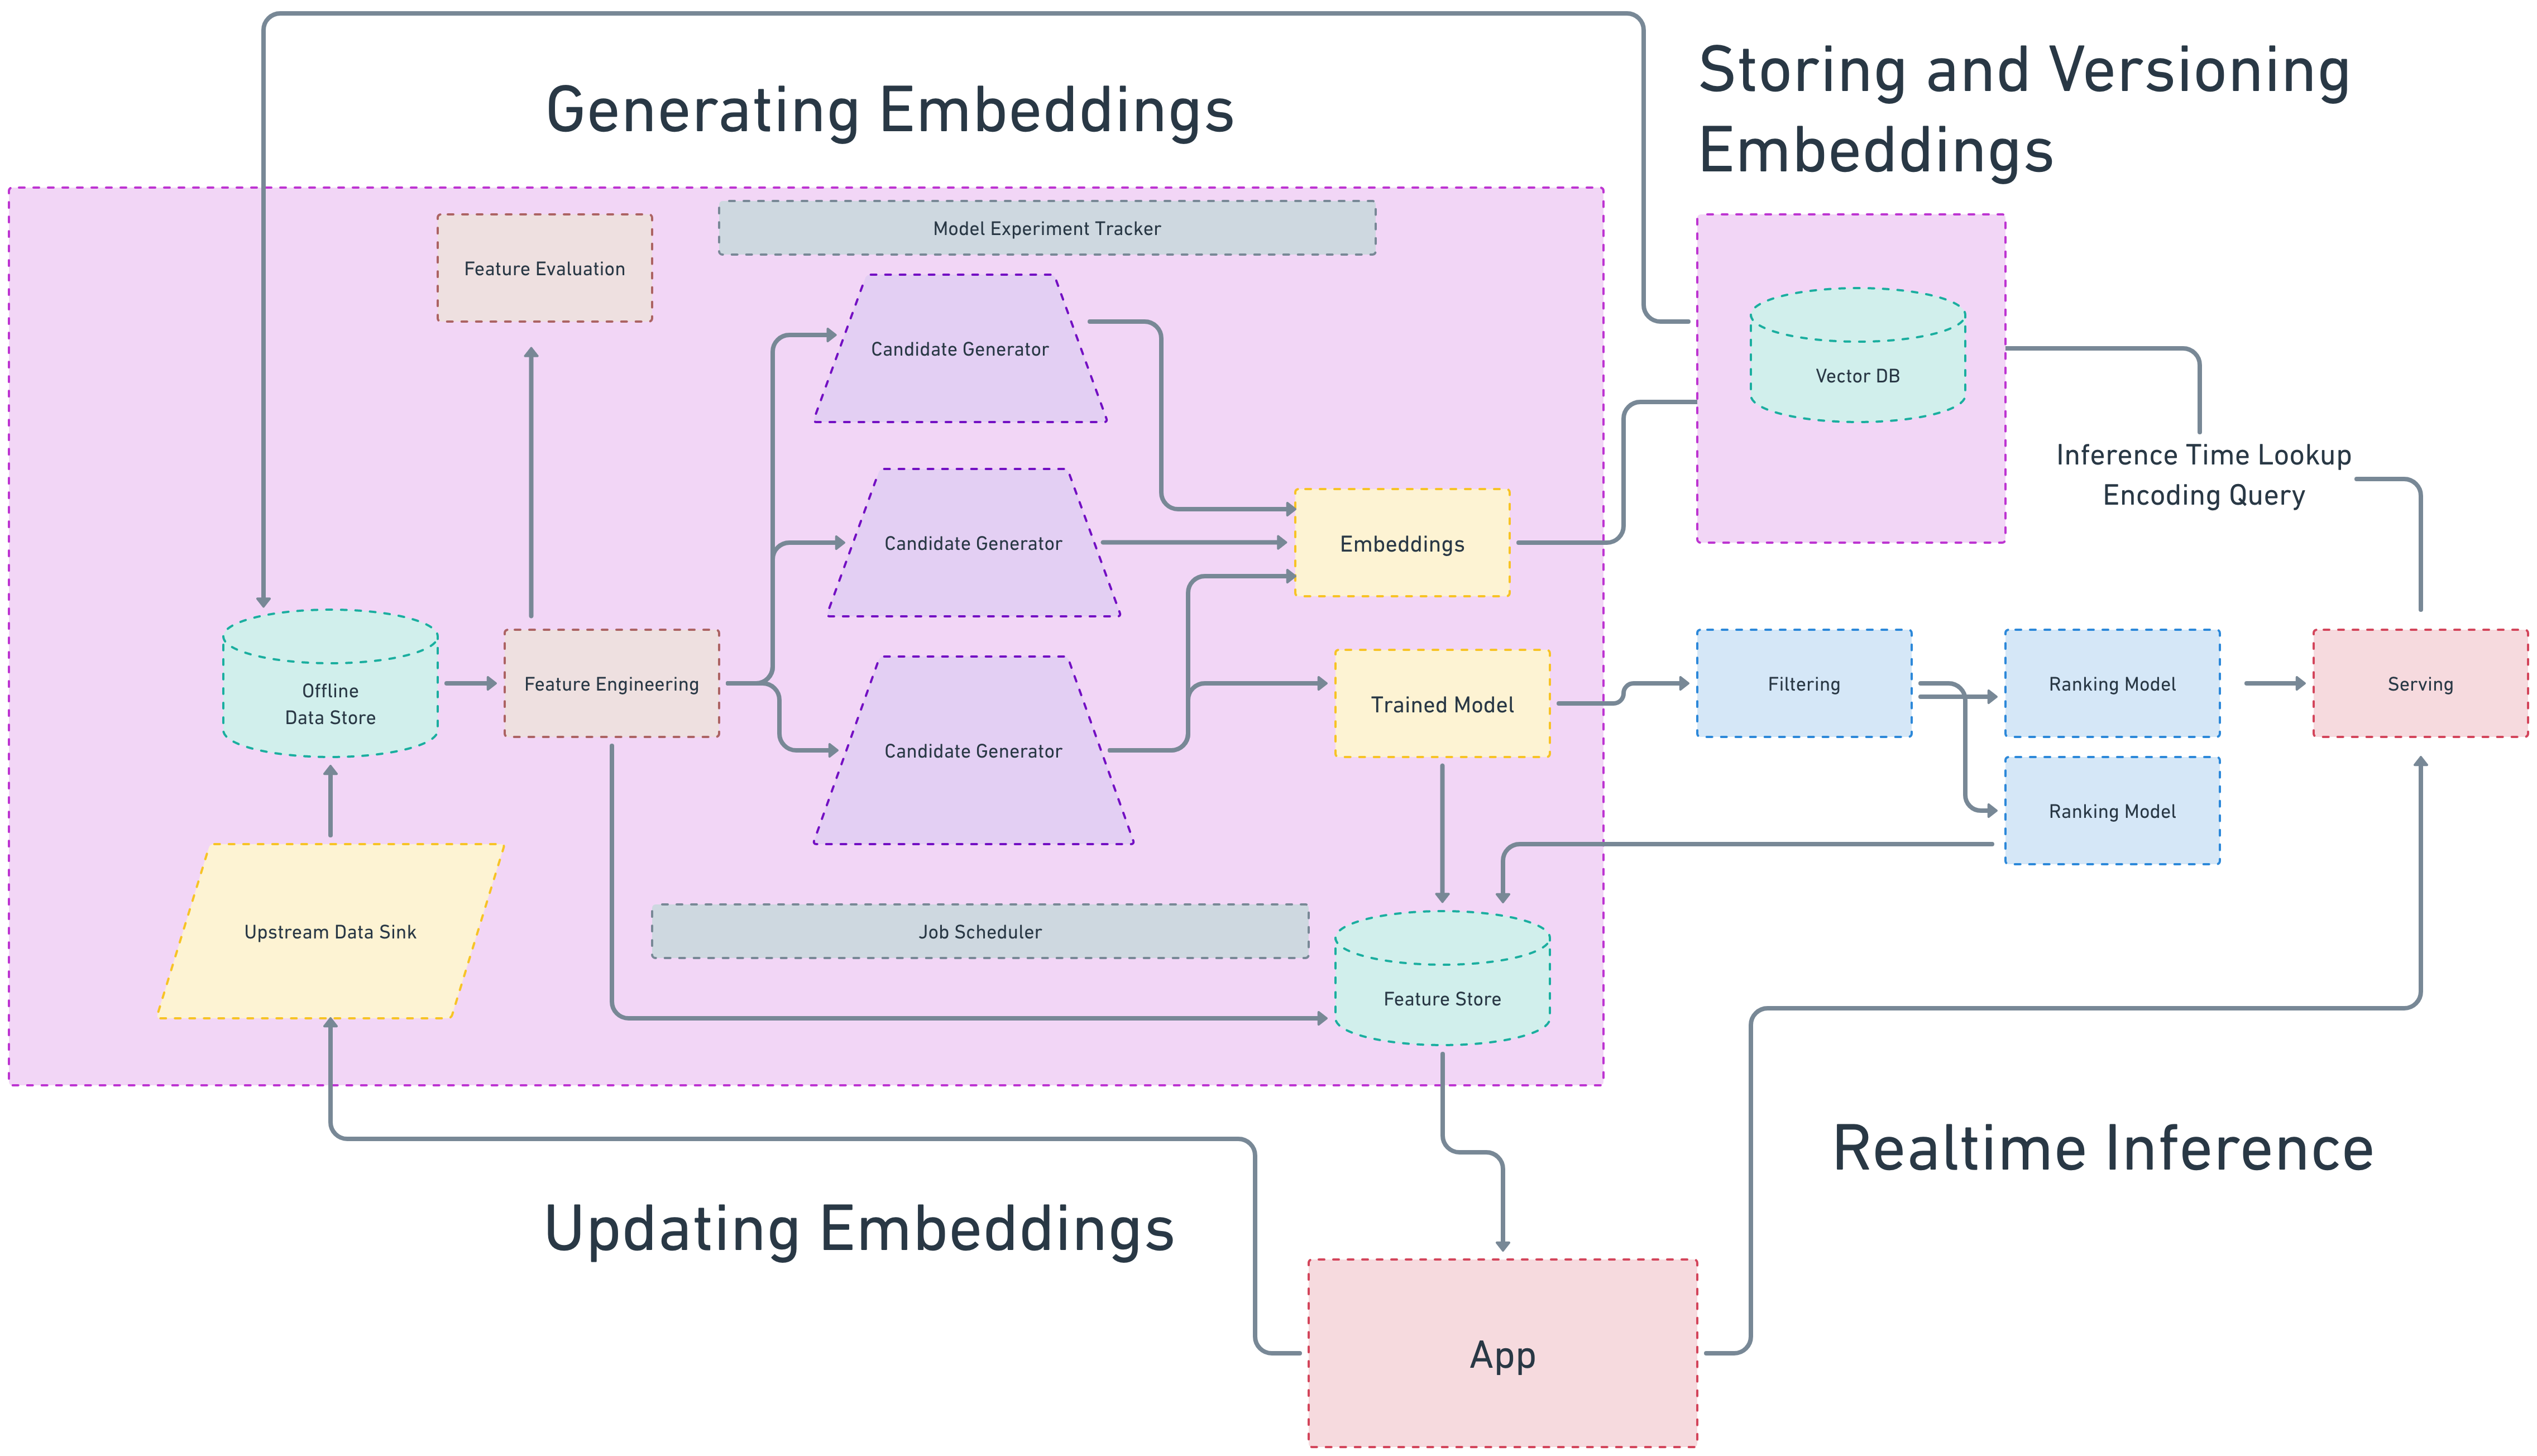
\includegraphics[width=\textwidth]{figures/embeddings_arch.png}
\caption{Recommender systems as a machine learning problem}
\end{figure}


\subsubsection{Embeddings Generation}

We've already seen that embeddings are usually generated as a byproduct of training neural network models, most often the penultimate layer that's used before a layer to classify or regress is added as the final output. We have two ways to build them. We can train our own models, as YouTube, Pinterest, and Twitter have done. In the LLM space, there is also \href{https://blog.replit.com/llm-training}{growing interest} in being able to train large language models in-house.

However, one of the large benefits of deep learning models is that we can also use pre-trained model. A pretrained model is any model that's like the one we're considering for our task that has already been trained on an enormous corpus of training data, and can be used for downstream tasks. \href{https://huggingface.co/docs/transformers/model_doc/bert}{BERT is an example} of a model that has already been pre-trained and can be used for any number of machine learning tasks through the process of \textbf{fine-tuning}. In fine-tuning, we take a model that's already been pre-trained on a generic dataset. For example, BERT was trained on \href{https://resources.wolframcloud.com/NeuralNetRepository/resources/BERT-Trained-on-BookCorpus-and-English-Wikipedia-Data}{BookCorpus, a set of 11k books with 800 million words and English Wikipedia, 2.5 billion words}.


\begin{formal}
\subsubsection*{An aside on training data}
Training data is the most important part of any given model. Where does it come from for pre-trained large language models? Usually scraping large parts of the internet. In the interest of competitive advantage, how these training datasets are put together is usually not revealed, and there is a fair amount of reverse-engineering and speculation. For example, \href{https://s10251.pcdn.co/pdf/2022-Alan-D-Thompson-Whats-in-my-AI-Rev-0.pdf}{"What's in my AI"} goes into the training data behind the GPT series of models and finds that GPT-3 was trained on Books1 and Books2. Books1 is \href{https://github.com/soskek/bookcorpus/issues/27#issuecomment-716104208}{likely bookcorpus} and books2 is likely \href{https://en.wikipedia.org/wiki/Library_Genesis}{libgen}. GPT also includes the Common Crawl, a large open-source dataset of indexed websites, WebText2, and Wikipedia. This information is important because when we pick  a model we need to at least understand at a high level what it was trained on to be a general-purpose model so we can explain what changes when we fine-tune it.
\end{formal}

In \textbf{fine-tuning} a model, we perform all the same steps as we do for training from scratch. We have training data, we have a model, and we minimize a loss function. However, there are several differences. When we create our new model, we copy the existing, pre-trained model with the exception of the final output layer, which we initialize from scratch based on our new task. When we train the model, we initialize these parameters at random and only continue to adjust the parameters of the previous layers so that they focus on this task rather than starting to train from scratch. In this way, if we have a model like BERT that's trained to generalize across the whole internet, but our corpus for Flutter is very sensitive to trending topics and needs to be updated on a daily basis, we can refocus the model without having to train a new one with as few as 10k samples instead of our original hundreds of millions \citep{zhang2020revisiting}.

There are, likewise, BERT embeddings available that we can fine-tune. There are other generalized corpuses available, such as GloVE, Word2Vec, and \href{https://fasttext.cc/docs/en/crawl-vectors.html}{FastText} (also trained with CBOW). We need to make a decision whether to use these, train a model from scratch, or a third option, to query \href{https://platform.openai.com/docs/guides/embeddings/limitations-risks}{embeddings available from an API} as is the case for OpenAI embeddings, although doing so can potentially come at a \href{https://github.com/ray-project/llm-numbers#101----cost-ratio-of-openai-embedding-to-self-hosted-embedding}{higher cost}, relative to training or fine-tuning our own. Of course, all of this is subject to our particular use-case and is important to evaluate when we start a project.

\subsubsection{Storage and Retrieval}

Once we've trained our model, we'll need to extract the embeddings from the trained object. Generally, when a model is trained, the resulting output is a data structure that contains all the parameters of the model, including the model's weights, biases, layers and learning rate. The embeddings are part of this model object as a layer, and they initially live in-memory. When we write the model to disk, we propagate them as a model object, which is serialized onto memory and loaded at re-training or inference time.

The simplest form of embedding store can be an in-memory numpy array\footnote{From a Tweet by Andrej Karpathy in response to how he stores vector embeddings for a small movie recommendations side project in 2023,"np.array people keep reaching for much fancier things way too fast these days. \href{https://twitter.com/karpathy/status/1647374645316968449}{Tweet}}.

 But if we are iterating on building a model with embeddings, we want to be able to do a number of things with them:

\begin{formal}
\begin{itemize}
  \item Access them in batch and one-by-one at inference time
  \item Perform offline analysis on the quality of the embeddings
  \item Embedding feature engineering
  \item Update embeddings with new models
  \item Version embeddings
   \item Encode new embeddings for new documents
\end{itemize}
\end{formal}

The most complex and customizable software that handles many of these use-cases is a vector database, and somewhere in-between vector databases and in-memory storage are vector searchplugins for existing stores like Postgres and SQLite, and caches like Redis.

The most important operation we'd like to perform with embeddings is vector search, which allows us to find embeddings that are similar to a given embedding so we can return item similarity. If we want to search embeddings, we need a mechanism that is optimized to search through our matrix data structures and perform nearest-neighbor comparisons in the same way that a traditional relational database is optimized to search row-based relations. Relational databases use a b-tree structure to optimize reads by sorting items in ascending order within a hierarchy of nodes, built on top of an indexed column in the database. We can't perform columnar lookups on our vectors efficiently, so we need to create different structures for them. For example, many vector stores are based on inverted indices.

A general-form embeddings store contains the embeddings themselves, an index to map them back from the latent space into words, pictures, or text, and a way to do similarity comparisons between different types of embeddings using various nearest neighbors algorithms. We talked before about \textbf{cosine similarity} as a staple of comparing latent space representations. This can become computationally expensive over millions of sets of vectors, because we'd need to do a pairwise comparison over every pair. To solve this, \textbf{approximate nearest neighbors (ANN)} algorithms were developed to, as in recommender systems, create neighborhoods out of elements of vectors and find a vector's k-nearest neighbors. The most frequently-used algorithms include \textbf{HNSW} (hierarchical navigable small worlds) and \textbf{Faiss}, both of which are standalone libraries and also implemented as part of many existing vector stores.

The trade-off between full and nearest neighbor search is that the latter is less precise, but it's much faster. When we switch between precision and recall in evaluation, we need to be aware of the tradeoffs and think about what our requirements are with respect to how accurate our embeddings are and their inference latency.

Here's an example of the embeddings storage system that Twitter built for exactly this use case, long before vector databases came into the picture.  \citep{shiebler2010making}.

\begin{figure}[H]
\centering{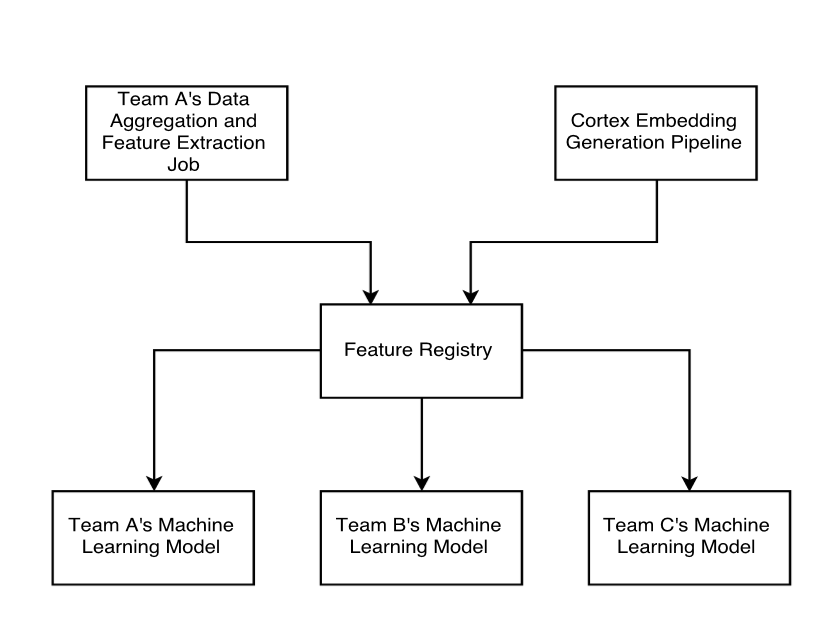
\includegraphics[width=.6\textwidth]{figures/embedding_pipeline.png}}
\caption{Twitter's embeddings pipeline \citep{shiebler2010making}}
\end{figure}

Given that Twitter uses embeddings in multiple sources as described in the previous section, Twitter made embeddings "first class citizens" by creating a centralized platform that reprocesses data and generates embeddings downstream into the feature registry.

\subsubsection{Drift Detection, Versioning, and Interpretability}

Once we've trained embeddings, we might think we're done. But embeddings, like any machine learning pipeline, need to be refreshed because we might run into \textbf{concept drift}. Concept drift occurs when the data underlying our model changes. For example, let's say that our model includes, as a binary feature, people who have landlines or not. In 2023, this would no longer be as relevant of a feature in most of the world as most people have switched to cell phones as their primary telephones, so the model would lose accuracy.

This phenomenon is even more prevalent with embeddings that are used for classification. For example, let's say we use embeddings for trending topic detection. The model has to generalize, as in the wide and deep model, to detect new classes, but if our classes change quickly, it may not be able to, so we need to retrain your embeddings frequently. Or, for example, if we model embeddings in a graph, as Pinterest does, and the relationships between nodes in the graph change, we may have to update them \citep{wewer2021updating}. We could also have an influx of spam or corrupted content which changes the relationship in your embeddings, in which case we'll need to retrain.

Embeddings can be hard to understand (so hard that some people have even written entire papers about them) and harder to interpret. What does it mean for a king to be close to queen but far away from the knight? What does it mean for two flits to be close to each other in a projected embedding space?  

We have two ways we can think about this, \textbf{intrinsic} and \textbf{extrinsic} evaluation. For the embeddings themselves (extrinsic evaluation), we can visualize them through either \textbf{UMAP}---Uniform Manifold Approximation and Projection for Dimension Reduction or \textbf{t-sne} --- t-distributed stochastic neighbor embedding, algorithms that allow us to visualize highly-dimensional data in two or three dimensions, much like PCA. Or we can fit embeddings into our downstream task (for example, summarization, or classification), and analyze the same way we would with offline metrics. There are many different approaches
 \citep{wang2019evaluating} but the summary is that embeddings can be objectively hard to evaluate and we'll need to factor the time to perform this evaluation into our modeling time.

Once we retrain our initial baseline model, we now have a secondary issue: how do we compare the first set of embeddings to the second; that is, how do we evaluate whether they are good representations of our data, given the case that embeddings are often unsupervised; i.e. --- how do we know whether "king" should be close to "queen"? On their own, as a first-pass, embeddings can be hard to interpret, because in a multidimensional space it's hard to understand which dimension of a vector corresponds to a decision to place items next to each other \citep{simhi2022interpreting}.  When compared to other sets of embeddings, we might use the offline metrics of the final model task, precision and recall, or we could measure the distance of the distribution of the embeddings in the latent space by comparing the statistical distance between the two probability distributions using a metric known as \textbf{Kullback–Leibler divergence}.

Finally, now let's say that we have two sets of embeddings, you need to version them and keep both sets so that, in case your new model doesn't work as well, you can fall back to the old one. This goes hand-in-hand with the problem of model versioning in ML operations, except in this case we need to both version the model and the output data.

There are numerous different approaches to model and data versioning that involve building a system that tracks both the metadata and the location of the assets that are kept in a secondary data store. Another thing to keep in mind is that embedding layers, particularly for large vocabularies, can balloon in size, so now we have to consider storage costs, as well.


\subsubsection{Inference and Latency}

When working with embeddings, we are operating not only in a theoretical, but practical engineering environment. The most critical engineering part of any machine learning system that works in production is inference time --- how quickly does it take to query the model asset and return a result to an end-user.

For this, we care about latency, which we can roughly define as any time spent waiting and is a critical performance metric in any production system \citep{gregg2014systems}. Generally speaking, it's the time of any operation to complete -- application request, database query, and so on. Latency at the level of the web service is generally measured in milliseconds, and every effort is made to reduce this as close to zero as realistically possible. For use-cases like search and loading a feed of content, the experience needs to be instantaneous or the user experience will degrade and we could even lose revenue. In a study from a while back, Amazon found that every 100ms increase in latency cuts profits by 1\%  \citep{flach2013reducing}.

Given this, we need to think about how to reduce the footprint of our model and all the layers in serving it so that the response to the user is instantaneous. We do this by creating observability throughout our machine learning system, starting with the hardware the system is running on, to CPU and GPU utilization, the performance of our model architecture, and how that model interacts with other components. For example, when we are performing nearest neighbor lookup, the way we perform that lookup and the algorithm we use, the programming language we use to write that algorithm, all compound latency concerns.  

As an example, in the wide and deep paper, the recommender ranking model scores over 10 million apps per second. The application was initially single-threaded, with all candidates taking 31 milliseconds. By implementing multithreading, they were able to reduce client-side latency to 14 milliseconds \citep{cheng2016wide}.

Operations of machine learning systems is an entirely other art and craft of study and one that's best left for another paper \citep{kreuzberger2022machine}.

\subsubsection{Online and Offline Model Evaluation}
We've barely scratched the surface of one of the most critical parts of a model: how it performs in offline and online testing. When we talk about offline tests, we mean analyzing the statistical properties of a model to learn whether the model is a valid model - i.e. does our loss function converge? Does the model overfit or underfit? What is the precision and recall? Do we experience any drift? If it's a recommendation ranker model, are we using metrics like \textbf{NDCG} ---normalized discounted cumulative gain--- to understand whether our new model ranks items better than the previous iteration?

Then, there is online evaluation, aka how successful the model actually is in the production context. Usually, this is evaluated through A/B testing where one set of users gets the old model or system and a holdout set of users gets the new system, and looking at the statistical significance of metrics like click-through rate, items served, and time spent on a given area of the site.

\subsubsection{What makes embeddings projects successful}
Finally, once we have all our algorithmic and engineering concerns lined up, there is the final matter to consider of what will make our project successful from a business perspective. We should acknowledge that we might not always need embeddings for our machine learning problem, or that we might not need machine learning at all, initially, if our project is based entirely on a handful of heuristic rules that can be determined and analyzed by humans \citep{zinkevich2017rules}.

If we conclude that we are operating in a data-rich space where automatically inferring semantic relationships between entities is correct, we need to ask ourselves if we're willing to put in a great deal of effort into producing clean datasets, the baseline of any good machine learning model, even in cases of large language models. In fact, clean, domain data is so important that many of the companies discussed here ended up training their own embeddings models, and, recently companies like Bloomberg \citep{wu2023bloomberggpt} and Replit \citep{Shabani_2023} are even training their own large language models to improve accuracy for their specific business domain.

Critically, to get to a stage where we have a machine learning system dealing with embeddings, we need a team that has multilevel alignment around the work that needs to be done. In larger companies, the size of this team will be larger, but most specifically work with embeddings requires someone who can speak to the use case specifically, someone who advocates for the use case and gets it prioritized, and a technical person who can do the work \citep{meil2023ai}.

If all of these components come together, we now have an embeddings-based recommender system in production.

%------------------------------------------------

\section{Conclusion}

We have now walked through an end-to-end example of what embeddings are. We started with a high-level overview of how embeddings fit into the context of a machine learning application. We then did a deep dive on early approaches to encoding, built up intuition of embeddings in Word2Vec and then moving on to transformers and BERT. Although reducing dimensionality as a concept has always been important in machine learning systems to decrease computational and storage complexity, compression has become even more important in the modern explosion of multimodal representations of data that comes from application log files, images, video, and audio, and the explosion of Transformer, generative, and diffusion models, combined with the cheap storage and explosion of data, has amended itself to architectures where embeddings are used more and more.

We've understood the engineering context of why we might include machine learning models in our application, how they work, how to incorporate them, and where embeddings ---dense representations of deep learning model input and output data -- can be best leveraged.  Embeddings are a powerful tool in any machine learning system, but one that comes at a cost of maintenance and interpretability. Generating embeddings using the correct method, with the correct metrics and hardware and software, is a project that takes considerable thought.  We now hopefully have a solid grasp of the fundamentals of embedding and can either leverage them -- or explain why not to --in our next project.
Good luck navigating embeddings, see you in the latent space!


\newpage

%----------------------------------------------------------------------------------------
%	BIBLIOGRAPHY
%----------------------------------------------------------------------------------------

\newpage
\bibliographystyle{plainnat}
\bibliography{embeddings.bib}

%----------------------------------------------------------------------------------------
\end{sloppypar}
\end{document}




